\documentclass[a4paper,11pt]{report}

\usepackage[utf8]{inputenc}
\usepackage[T1]{fontenc}
\usepackage[italian]{babel}
\usepackage{lmodern}      % Latin Modern — versione vettoriale uniforme di Computer Modern
\usepackage{geometry}
\usepackage{booktabs}
\usepackage{longtable}
\usepackage{array}
\usepackage[table]{xcolor}
\usepackage{colortbl}
\usepackage{graphicx}
\usepackage{hyperref}
\usepackage{parskip}
\usepackage{enumitem}
\usepackage{fancyhdr}
\usepackage{titlesec}
\titleformat{\chapter}[hang]{\LARGE\bfseries}{}{0pt}{}
\titleformat{\section}[hang]{\normalfont\Large\bfseries}{}{0pt}{}
\titlespacing*{\chapter}{0pt}{0pt}{0.8em}
\usepackage{caption}
\usepackage{float}
\usepackage{lscape}
\usepackage{pdflscape}
\usepackage{pdfpages}
\usepackage{microtype}
\usepackage{tabularx}
\usepackage{multirow}
\usepackage{needspace}
\usepackage[normalem]{ulem} % \uline: sottolineatura che va a capo correttamente (a differenza di \underline)

\geometry{margin=1.8cm}

\setlength{\arrayrulewidth}{0.8pt}
\arrayrulecolor{black}

\graphicspath{{img/}}

\hypersetup{
    colorlinks=true,
    linkcolor=black,
    urlcolor=blue,
    citecolor=blue,
    pdfauthor={SAS 2025/26},
    pdftitle={Gestire gli eventi -- Cat \& Ring}
}

% Header/footer
\pagestyle{fancy}
\fancyhf{}
\fancyfoot[C]{}
\renewcommand{\headrulewidth}{0pt}
% Le pagine di apertura capitolo usano lo stile "plain" di default (report),
% che altrimenti mostrerebbe comunque il numero di pagina in fondo.
\fancypagestyle{plain}{%
  \fancyhf{}%
  \renewcommand{\headrulewidth}{0pt}%
  \renewcommand{\footrulewidth}{0pt}%
}

% Colors
\definecolor{headerblue}{RGB}{30,80,150}
\definecolor{rowgray}{RGB}{240,240,240}
\definecolor{actorgreen}{RGB}{220,240,220}
\definecolor{sysblue}{RGB}{220,230,245}

% Column types
\newcolumntype{L}[1]{>{\raggedright\arraybackslash}p{#1}}
\newcolumntype{C}[1]{>{\centering\arraybackslash}p{#1}}

% ── UC Cockburn — 3 colonne: # | Attore | Sistema ──────────────
% \ucstep{n}{attore}{sistema}    passo normale
% \ucexstep{n}{attore}{sistema}  passo eccezione (n in rosso)
% \ucflow{testo}                 riga corsivo span 3 col (loop/branch/"Termina")
% \extensionhead{titolo}         intestazione estensione (grassetto grande)
% \exceptionhead{titolo}         intestazione eccezione  (grassetto rosso grande)
% \uctablebegin / \uctableend    apre/chiude la longtable

\newcommand{\ucstep}[3]{\textbf{#1} & #2 & #3 \\* \hline}
\newcommand{\ucexstep}[3]{\textcolor{red}{\textbf{#1}} & #2 & \cellcolor{red!20}#3 \\* \hline}
\newcommand{\ucflow}[1]{%
  \multicolumn{3}{|L{14.0cm}|}{\itshape #1} \\* \hline}

\newcommand{\extensionhead}[1]{%
  \Needspace{8\baselineskip}%
  \vspace{0.5em}\par\noindent{\Large\textbf{#1}}\par\vspace{0.15em}}
\newcommand{\exceptionhead}[1]{%
  \Needspace{8\baselineskip}%
  \vspace{0.5em}\par\noindent{\Large\textcolor{red}{\textbf{#1}}}\par\vspace{0.15em}}

\newcommand{\uctablebegin}{%
  \renewcommand{\arraystretch}{1.5}%
  \begin{longtable}{|C{1.5cm}|L{6.25cm}|L{6.25cm}|}
  \hline
  \rowcolor{actorgreen}%
  \textbf{\#} &
  \textbf{Attore} &
  \textbf{Sistema} \\ \hline
  \endfirsthead
  \hline
  \endhead
  \endfoot
}
\newcommand{\uctableend}{\end{longtable}\renewcommand{\arraystretch}{1.0}}

% Contract environment
\newenvironment{contratto}[1]{%
  \subsubsection*{\parbox[t]{\linewidth}{\raggedright\Large\bfseries #1}}
  \begin{description}[leftmargin=3cm, labelwidth=2.8cm, labelsep=0.2cm]
}{%
  \end{description}
  \vspace{0.5em}
}
\newcommand{\cpre}[1]{\item[Pre-condizioni:] #1}
\newcommand{\cpost}[1]{\item[Post-condizioni:] #1}

% Convenzioni tipografiche dei contratti (stile Larman):
%   \cobj{}   istanza/oggetto già legato (non un parametro dell'operazione)
%   \cparam{} parametro formale dell'operazione, ovunque sia referenziato
%   \crel{}   relazione, ruolo o verbo logico del modello di dominio
\newcommand{\cobj}[1]{\textit{#1}}
\newcommand{\cparam}[1]{\uline{#1}}
\newcommand{\crel}[1]{\textbf{#1}}

%───────────────────────────────────────────────
\begin{document}

%--- Title page
\begin{titlepage}
  \centering
  \vspace*{2cm}
  {\huge\bfseries Sviluppo delle Applicazioni Software\\Laboratorio\par}
  \vspace{0.5cm}
  {\LARGE a.a 2025/2026\par}
  \vspace{2cm}
  {\LARGE\bfseries Gestione degli Eventi\par}
  \vfill
  {\LARGE Alessandra Tilloca --- 1098173\par}
  \vspace{0.3cm}
  {\LARGE Elis Qose --- 1094455\par}
  \vfill
\end{titlepage}

\chapter{Glossario}

% ─── Attori ───────────────────────────────────────────────────
\section*{Attori}

\begin{longtable}{L{3.5cm} L{8.5cm} L{3cm}}
\toprule
\textbf{Termine} & \textbf{Descrizione} & \textbf{Sinonimi} \\
\midrule
\endhead
\bottomrule
\endfoot

Chef
& Stabilisce il \textbf{menù} per gli \textbf{eventi} e ne supervisiona
  la preparazione.
& — \\
\addlinespace

Cliente
& Colui che commissiona l'organizzazione di un \textbf{evento}.
& — \\
\addlinespace

Cuoco
& Prepara il \textbf{cibo}.
& — \\
\addlinespace

Organizzatore
& La persona che gestisce il \textbf{personale} e gli \textbf{eventi}.
& — \\
\addlinespace

Personale
& La parola \emph{personale} è usata in modo ambiguo nel testo per intendere
  talvolta tutti i dipendenti (\textbf{chef}, \textbf{cuochi},
  \textbf{personale di servizio}), talvolta soltanto i dipendenti soggetti
  a \textbf{turni} (\textbf{cuochi} e \textbf{personale di servizio}).
  In presenza di questo termine consultare il cliente per disambiguare.
& — \\
\addlinespace

Personale di Servizio
& Le persone (maître e camerieri) che si occupano del \textbf{servizio}
  durante l'\textbf{evento} stesso.
& Staff di supporto \\
\addlinespace

Utente
& Generico utilizzatore dell'applicazione (ha necessariamente un ruolo fra
  \textbf{organizzatore}, \textbf{chef}, \textbf{cuoco},
  \textbf{personale di servizio}).
& — \\

\end{longtable}

% ─── Dominio ──────────────────────────────────────────────────
\section*{Dominio dell'Applicazione}

\begin{longtable}{L{3.5cm} L{8.5cm} L{3cm}}
\toprule
\textbf{Termine} & \textbf{Descrizione} & \textbf{Sinonimi} \\
\midrule
\endhead
\bottomrule
\endfoot

Annullamento di un evento
& Un \textbf{evento} può essere annullato in qualsiasi fase della sua
  predisposizione. Se l'annullamento avviene a ridosso della data
  dell'\textbf{evento} (tipicamente a meno di una settimana), al
  \textbf{cliente} viene addebitata una \textbf{penale}.
& — \\
\addlinespace

Autore (di una ricetta)
& Chi ha ideato la \textbf{ricetta}.
& — \\
\addlinespace

Capofila (di un evento ricorrente)
& L'\textbf{evento ricorrente} da cui le singole \textbf{istanze}
  ereditano le impostazioni di default (luogo, durata, numero di
  servizi richiesti, numero di partecipanti, note e cliente). Le modifiche al
  capofila possono essere propagate a tutte le istanze ancora
  modificabili; ogni \textbf{istanza} può tuttavia essere modificata
  individualmente senza alterare le altre.
& — \\
\addlinespace

Cibo
& Piatti preparati (seguendo una \textbf{ricetta} del \textbf{ricettario})
  per essere consumati durante un \textbf{servizio}.
& Pietanze \\
\addlinespace

Compito (di cucina)
& Attività assegnata dallo \textbf{chef} ai \textbf{cuochi} durante la fase
  di \textbf{lavoro preparatorio}, che consiste nello svolgimento di uno o
  più \textbf{passi} di una \textbf{ricetta} o \textbf{preparazione} volti
  alla realizzazione di un \textbf{piatto} o di un \textbf{preparato
  intermedio} in vista di un \textbf{servizio} che deve essere effettuato.
& — \\
\addlinespace

Conclusione (di un evento ricorrente)
& La data fino a cui l'\textbf{evento ricorrente} si ripete, oppure un
  numero massimo di ripetizioni che avranno luogo.
& — \\
\addlinespace

Disponibilità
& Indicazione fornita da un \textbf{cuoco} o dal \textbf{personale di
  servizio} riguardo la propria presenza per un \textbf{turno}. La
  disponibilità può essere revocata finché la persona non viene
  effettivamente convocata/assegnata al turno da \textbf{chef} od
  \textbf{organizzatore}, momento in cui diventa un vincolo non più
  ritirabile.
& — \\
\addlinespace

Documentazione
& Informazioni e allegati inseriti dall'\textbf{organizzatore} al momento
  del passaggio dell'\textbf{evento} allo stato \emph{terminato}.
& Note di chiusura \\
\addlinespace

Dose (di un ingrediente)
& Indica la quantità di ogni \textbf{ingrediente} (di base o preparati)
  necessario alla preparazione di un \textbf{piatto}.
& — \\
\addlinespace

Eliminazione di un evento
& Rimozione definitiva della \textbf{scheda di un evento} e di tutti i suoi
  dati. Un \textbf{evento} può essere eliminato solo quando si trova in
  stato di \emph{bozza}, ossia prima che i \textbf{menù} vengano
  approvati e i lavori abbiano inizio. Una volta che l'\textbf{evento}
  è \emph{in corso} non è più eliminabile, ma può essere
  \textbf{annullato} (si veda \emph{annullamento di un evento}).
& — \\
\addlinespace

Evento
& Contesto in cui viene fornito il \textbf{servizio} di catering. Prevede due
  momenti diversi: il \textbf{lavoro preparatorio} e il \textbf{servizio}.
  Se ne fa carico un \textbf{organizzatore}, mentre la cucina è affidata a
  uno \textbf{chef}.
  Un evento può essere \emph{semplice}, e prevedere un singolo \textbf{servizio},
  o \emph{complesso}, prevedendo più \textbf{servizi} (pranzo e cena, colazione
  e pranzo, coffee-break mattino e pomeriggio, ecc.) in una o più giornate.
  Un evento attraversa i seguenti stati:
  \begin{itemize}[nosep,leftmargin=*]
    \item \emph{bozza}: l'\textbf{organizzatore} sta definendo la
          \textbf{scheda di un evento}; l'evento è eliminabile;
    \item \emph{in corso}: i \textbf{menù} sono stati approvati e i lavori
          hanno avuto inizio; l'evento non è più eliminabile, ma può essere
          annullato;
    \item \emph{terminato}: l'\textbf{organizzatore} ha chiuso l'evento al
          termine del \textbf{servizio};
    \item \emph{annullato}: l'evento è stato interrotto prima della sua
          conclusione naturale (si veda \textbf{annullamento di un evento}).
  \end{itemize}
& — \\
\addlinespace

Evento ricorrente
& \textbf{Evento} che si ripete con una data regolarità. In particolare è
  rilevante:
  \begin{itemize}[nosep,leftmargin=*]
    \item ogni quanto l'evento si ripete (\textbf{frequenza});
    \item la data fino a cui si ripete, o il numero di occorrenze
          (\textbf{conclusione}).
  \end{itemize}
& — \\
\addlinespace

Frequenza di un evento ricorrente
& Intervallo di tempo dopo cui l'\textbf{evento ricorrente} si ripete.
& — \\
\addlinespace

Gestione del servizio
& La gestione dei \textbf{servizi} che compongono un \textbf{evento} viene
  affidata a un \textbf{organizzatore}. Essa prevede:
  \begin{itemize}[nosep,leftmargin=*]
    \item scegliere il \textbf{personale di servizio} per ogni
          \textbf{turno di servizio} associato all'\textbf{evento},
          indicando il \textbf{ruolo} che avrà in quella particolare
          situazione;
    \item opzionalmente, l'assegnamento di un \textbf{cuoco} a quello stesso
          \textbf{servizio} se il \textbf{menù} prevede \textbf{ricette}
          che lo rendono necessario.
  \end{itemize}
& — \\
\addlinespace

Ingrediente
& Materia prima per preparare un \textbf{piatto}. Può essere \emph{di base}
  (scelto da un elenco di partenza corrispondente a ciò che si trova in
  dispensa) oppure un \textbf{preparato intermedio} realizzato in cucina
  dagli stessi \textbf{cuochi}.
& — \\
\addlinespace

Insieme delle istruzioni (di una ricetta)
& Spiegazione di come trasformare gli \textbf{ingredienti} di partenza in un
  prodotto finito. Sono divise in due sezioni: la parte realizzabile in
  anticipo e quella da realizzare all'ultimo sul posto dell'evento. Ogni
  singola istruzione è rappresentata da un \textbf{passo}.
& — \\
\addlinespace

Istanza (di evento)
& Singola edizione di un \textbf{evento ricorrente}. Di default
  eredita le impostazioni del \textbf{capofila}, ma può essere
  modificata individualmente senza influenzare le altre istanze
  della ricorrenza.
& Occorrenza \\
\addlinespace

Lavoro di servizio
& Momento di lavoro che si svolge nel luogo dell'\textbf{evento}, effettuato
  dal \textbf{personale di servizio} e opzionalmente da \textbf{cuochi} di
  supporto. È organizzato in \textbf{turni di servizio}.
& — \\
\addlinespace

Lavoro preparatorio
& Momento di lavoro che si svolge in \textbf{sede}, effettuato dai
  \textbf{cuochi} sotto la supervisione di uno \textbf{chef}. È organizzato
  in \textbf{turni preparatori}.
& Preparazione in sede \\
\addlinespace

Menù
& Descrive quali piatti vengono proposti in un dato \textbf{servizio}
  (nell'ambito di un \textbf{evento}). Si compone di diverse \textbf{voci},
  opzionalmente organizzate in \textbf{sezioni}. Lo \textbf{chef} costruisce
  i suoi menù a partire dalle \textbf{ricette} del \textbf{ricettario}.
  Un menù è caratterizzato da informazioni aggiuntive:
  \begin{itemize}[nosep,leftmargin=*]
    \item se è consigliata la presenza di un \textbf{cuoco} durante il
          \textbf{servizio};
    \item se prevede solo piatti freddi o anche piatti caldi;
    \item se richiede la disponibilità di una cucina nella \textbf{sede}
          dell'\textbf{evento};
    \item se è adeguato per un buffet;
    \item se può essere fruito senza posate (finger food).
  \end{itemize}
  Un menù può essere modificato fintanto che non è utilizzato in alcun
  \textbf{evento}.
& — \\
\addlinespace

Modifica al menù (di un evento)
& Variazione temporanea proposta dall'\textbf{organizzatore} prima
  dell'approvazione del \textbf{menù} per un \textbf{evento} (aggiungendo o
  togliendo piatti). Tali modifiche non alterano il \textbf{menù} originale
  presente nel \textbf{ricettario}, restano visibili come aggiunte o
  eliminazioni limitate all'\textbf{evento} in questione e devono essere
  confermate dallo \textbf{chef}.
& Proposta di modifica al menù \\
\addlinespace

Passo
& Singolo elemento che compone le istruzioni di una \textbf{ricetta}. I passi
  si dividono in due sezioni: quella dei passi realizzabili in anticipo
  (durante il \textbf{lavoro preparatorio}) e quella dei passi da effettuare
  sul posto (durante il \textbf{servizio}).
& Istruzione \\
\addlinespace

Penale
& Sanzione economica addebitata al \textbf{cliente} in caso di
  \textbf{annullamento di un evento} tardivo (tipicamente a meno di una
  settimana dall'evento) oppure di modifica sostanziale del numero di
  partecipanti dopo l'avvio dei lavori. L'\textbf{organizzatore} può, a
  propria discrezione, concedere deroghe (esenzioni) dalla penale a
  clienti affezionati.
& — \\
\addlinespace

Piatto
& Risultato dell'esecuzione di una \textbf{ricetta}, che può essere servito al
  \textbf{cliente} in quanto nel suo stato finale.
& — \\
\addlinespace

Porzione
& Quantità indicativa di un \textbf{piatto} finito per una persona.
& — \\
\addlinespace

Preparato intermedio
& Composto realizzato tramite le indicazioni di una \textbf{preparazione}, che
  diventa \textbf{ingrediente} di un'altra \textbf{preparazione} o di una
  \textbf{ricetta}.
& Preparato di base \\
\addlinespace

Preparazione (nel ricettario)
& Del tutto analoga a una \textbf{ricetta}, ma descrive come realizzare un
  \textbf{preparato intermedio} da utilizzare in un'altra \textbf{preparazione}
  o \textbf{ricetta}. Attraversa gli stessi stati di una \textbf{ricetta}:
  \begin{itemize}[nosep,leftmargin=*]
    \item \emph{bozza}: visibile solo al creatore; modificabile ed
          eliminabile;
    \item \emph{pubblicata}: visibile a tutti; non più modificabile se in
          uso, ritirabile solo se non utilizzata.
  \end{itemize}
& — \\
\addlinespace

Procedura (di preparazione)
& Sequenza di \textbf{passi} indicata da una \textbf{ricetta} (o
  \textbf{preparazione}) che un \textbf{cuoco} deve eseguire per realizzare
  il \textbf{piatto} o il \textbf{preparato intermedio}.
& — \\
\addlinespace

Proprietario (di una ricetta)
& Chi ha inserito la \textbf{ricetta} nel \textbf{ricettario}.
& — \\
\addlinespace

Raggruppamento di turni
& Insieme di uno o più \textbf{turni preparatori} per cui il
  \textbf{personale} fornisce un'unica \textbf{disponibilità}, valida per
  tutti i turni del raggruppamento o per nessuno; le regole di modifica
  della disponibilità si applicano all'intero raggruppamento. Può essere
  \emph{singolo} (raggruppa due o più turni specifici una tantum) o \emph{ricorrente}
(raggruppa turni che si ripetono con una data periodicità nel tempo).
& — \\
\addlinespace

Ricetta
& Descrive come preparare un \textbf{piatto} da servire a tavola a partire
  dagli \textbf{ingredienti} (ciascuno con una propria \textbf{dose}) e dalle
  istruzioni per realizzarla. È caratterizzata da un nome, da un
  \textbf{proprietario}, opzionalmente da un \textbf{autore}, e può essere
  accompagnata da una descrizione breve. Ha inoltre un tempo di preparazione
  e può essere accompagnata da tag (vegetariana, senza latticini, senza uova,
  senza glutine, vegana).
  Produce un \textbf{piatto} finito (a differenza di una \textbf{preparazione},
  che produce un \textbf{preparato intermedio}).
  Attraversa i seguenti stati:
  \begin{itemize}[nosep,leftmargin=*]
    \item \emph{bozza}: visibile solo al creatore; modificabile ed
          eliminabile;
    \item \emph{pubblicata}: visibile a tutti; non più modificabile se in
          uso, ritirabile solo se non utilizzata.
  \end{itemize}
& — \\
\addlinespace

Ricettario
& Un elenco/raccolta di \textbf{ricette} e \textbf{preparazioni}.
& — \\
\addlinespace

Richiesta (di organizzazione)
& Un \textbf{cliente} commissiona l'organizzazione di un \textbf{evento}
  all'azienda di catering.
& — \\
\addlinespace

Ruolo
& Specifica mansione assegnata a un membro del \textbf{personale di servizio}
  in un dato \textbf{servizio}.
& — \\
\addlinespace

Scheda di un evento
& Creata dall'\textbf{organizzatore}, è il documento in cui sono descritte le
  caratteristiche dell'\textbf{evento}. Riporta informazioni quali:
  \begin{itemize}[nosep,leftmargin=*]
    \item luogo;
    \item date;
    \item durata;
    \item numero di persone;
    \item numero di \textbf{servizi};
    \item \textbf{cliente}/committente;
    \item note particolari (opzionale).
  \end{itemize}
& — \\
\addlinespace

Sede
& Ubicazione della società di catering e delle relative cucine.
& — \\
\addlinespace

Sede di un evento
& Luogo di svolgimento degli \textbf{eventi}.
& — \\
\addlinespace

Servizio
& Attività che consiste nel servire ai partecipanti i piatti e le bevande
  preparati. Include l'allestimento preliminare e il rigoverno al termine.
  Può andare dal semplice buffet all'allestimento di una sala ristorante.
  Uno stesso \textbf{evento} può prevedere più servizi, anche in
  \textbf{sedi} diverse. Ciascun servizio avrà una precisa fascia oraria,
  e un proprio \textbf{menù} e un proprio \textbf{personale di servizio}.
  Un singolo servizio appartenente a un \textbf{evento} può essere
  annullato indipendentemente dagli altri servizi, assumendo lo stato di
  \emph{annullato} per permettere di liberare il personale assegnato.
& — \\
\addlinespace

Sezione di un menù
& Partizionamento (opzionale) di un \textbf{menù}. Ad esempio: primi,
  secondi, dolci sono sezioni.
& — \\
\addlinespace

Turno
& Periodo di attività di una persona caratterizzato da una data, un luogo di
  svolgimento e da una fascia oraria. I turni sono di due tipi:
  \textbf{turni preparatori} e \textbf{turni di servizio}. Un turno può
  essere indicato come ``completo'' se la cucina e lo staff per quel turno
  sono completamente impegnati.
& — \\
\addlinespace

Turno preparatorio
& \textbf{Turno} in cui i \textbf{cuochi} lavorano a preparare le pietanze.
  I turni preparatori possono essere raggruppati in un
  \textbf{raggruppamento di turni}: il \textbf{personale} dà la propria
  \textbf{disponibilità} per tutti i turni del raggruppamento o per nessuno.
& Turno di cucina \\
\addlinespace

Turno di servizio
& \textbf{Turno} in cui lavorano il \textbf{personale di servizio} e i
  \textbf{cuochi} per realizzare il \textbf{servizio} stesso. Può
  specificare un tempo aggiuntivo rispetto agli orari del \textbf{servizio}
  effettivo per la preparazione (prima) e per rigovernare (dopo).
& — \\
\addlinespace

Voce di un menù
& Singolo elemento di un \textbf{menù}. Può appartenere a una \textbf{sezione}
  se il \textbf{menù} è diviso in sezioni. Ogni voce fa riferimento a una
  \textbf{ricetta} nel \textbf{ricettario}, ma il testo della voce può essere
  diverso dal nome della \textbf{ricetta}.
& — \\

\end{longtable}


\chapter{Caso d'Uso Dettagliato}

\section*{Informazioni generali}

\renewcommand{\arraystretch}{1.4}
\begin{tabular}{L{4.5cm} L{9.5cm}}
\toprule
\textbf{Nome caso d'uso}             & Gestire gli eventi \\
\textbf{Portata}                     & Sistema \\
\textbf{Livello}                     & Obiettivo utente \\
\textbf{Attore primario}             & Organizzatore \\
\textbf{Parti interessate}           & Chef, Cuoco, Personale di servizio, Cliente \\
\midrule
\textbf{Pre-condizioni}              & L'attore è autenticato come Organizzatore. \\
\textbf{Garanzie di Successo o Post-Condizioni} & L'evento è registrato con scheda evento
                                       compilata, chef assegnato, menù approvati
                                       e personale scelto per i turni di servizio. \\
\bottomrule
\end{tabular}
\renewcommand{\arraystretch}{1.0}

\extensionhead{Scenario principale di successo}

\uctablebegin
  \ucstep{1}
    {Crea una nuova scheda evento specificando: luogo, data di inizio, durata, numero
    di servizi richiesti, numero di partecipanti, note e cliente committente.}
    {Registra la scheda evento nello stato \emph{bozza}, senza ancora
     alcun servizio associato.}

  \ucstep{2}
    {Opzionalmente verifica lo stato della cucina.}
    {Fornisce gli impegni della cucina nei giorni richiesti dall'evento.}

  \ucstep{3}
    {Aggiunge un servizio specificando: tipo di servizio, data (rispetto
     all'inizio dell'evento), ora di inizio, ora di fine e numero di
     commensali.}
    {Registra il nuovo servizio, associandolo all'evento.}

  \ucstep{4}
    {Opzionalmente inserisce il turno di servizio corrispondente al
     servizio appena creato, specificando il tempo aggiuntivo di
     preparazione (prima) e di rigoverno (dopo) rispetto alla fascia
     oraria del servizio.}
    {Registra il turno di servizio, calcolando gli orari a partire
     dalle ore di inizio e fine del servizio e dai tempi aggiuntivi
     indicati.}

  \ucflow{Ripete i passi~3 e~4 per ogni servizio dell'evento (almeno una volta).}

  \ucstep{5}
    {Assegna uno chef all'evento.}
    {Registra l'assegnazione dello chef.}

  \ucstep{6}
    {Consulta il menù proposto dallo chef per il servizio.}
    {Fornisce il menù proposto per il servizio.}

  \ucstep{7}
    {Opzionalmente approva il menù.}
    {Registra l'approvazione. Quando i menù di tutti i servizi
     dell'evento sono stati approvati, l'evento passa allo stato
     \emph{in corso}. L'evento non è più eliminabile, ma può essere
     annullato.}

  \ucflow{Ripete i passi~6 e~7 per ogni servizio dell'evento.}

  \ucstep{8}
    {Sceglie il personale per il turno indicando il ruolo
     di ciascun membro.}
    {Registra le assegnazioni di ruolo per il turno.}

  \ucflow{Ripete il passo~8 per ogni turno di servizio dell'evento.}

  \ucstep{9}
    {Chiude l'evento aggiungendo note finali e allegando eventuale
     documentazione.}
    {Registra l'evento nello stato \emph{terminato}.}

  \ucflow{Termina il caso d'uso.}
\uctableend

% ─── Eccezione 1a ───────────────────────────────────────────
\exceptionhead{Eccezione 1a}

\uctablebegin
  \ucexstep{1a.1}
    {Specifica una data di inizio a meno di due settimane dalla data
     corrente (soglia maggiore, a discrezione dell'organizzatore, per
     eventi di grandi dimensioni --- 50 o più partecipanti --- o che
     si estendono su più giornate).}
    {Segnala che il preavviso non è sufficiente per accettare la
     commessa e richiede l'inserimento di una data valida.}
  \ucflow{Torna al passo~1 (l'attore modifica la data e riprova).}
\uctableend

% ─── Estensione 1b ──────────────────────────────────────────
\extensionhead{Estensione 1b}

\uctablebegin
  \ucstep{1b.1}
    {Invece di creare un nuovo evento, seleziona una scheda evento già
     esistente (in stato \emph{bozza}, \emph{in corso}, \emph{terminato}
     o \emph{annullato}).}
    {Fornisce la scheda dell'evento con i dati e lo stato corrente.}
  \ucflow{L'attore sceglie tra:
    \begin{itemize}[nosep,leftmargin=1.2em]
      \item Semplice consultazione $\to$ Termina il caso d'uso.
      \item Riprendere la pianificazione $\to$ Prosegue al passo~2.
      \item Modificare i dati $\to$ Vai all'Estensione~1d.
      \item Eliminare l'evento $\to$ Vai all'Estensione~1e.
      \item Annullare l'evento $\to$ Vai all'Estensione~1f.
    \end{itemize}}
\uctableend

% ─── Estensione 1c ──────────────────────────────────────────
\newpage
\extensionhead{Estensione 1c}

\uctablebegin
  \ucstep{1c.1}
    {Specifica che l'evento è ricorrente, indicando la frequenza e,
     in alternativa, la data di conclusione oppure il numero di
     occorrenze.}
    {Crea il capofila e tutte le istanze corrispondenti alla ricorrenza
     (ancora senza servizi). Finché il capofila è in fase di
     costruzione, le istanze condividono le sue stesse
     impostazioni di default; sono comunque visibili e modificabili
     singolarmente fin da subito.}
  \ucflow{Prosegue al passo~2.}
\uctableend

% ─── Estensione 1d ──────────────────────────────────────────
\extensionhead{Estensione 1d}

\uctablebegin
  \ucstep{1d.1}
    {Se l'evento è in stato \emph{bozza}: modifica luogo, data di
     inizio, durata, numero di servizi richiesti, numero di partecipanti,
        cliente, note, oppure aggiunge o rimuove un servizio.}
    {Registra le modifiche consentite per lo stato corrente.}
  \ucstep{1d.2}
    {Se l'evento è in stato \emph{in corso}: modifica solo il numero di
     partecipanti o le note.}
    {Registra le modifiche consentite per lo stato corrente.}
  \ucflow{Prosegue al passo~2.}
\uctableend

\exceptionhead{Eccezione 1d.1a}

\uctablebegin
  \ucexstep{1d.1a.1}
    {Tenta di modificare un evento nello stato \emph{annullato} o
     \emph{terminato}.}
    {L'evento non è più modificabile. Segnala l'errore.}
  \ucflow{Termina il caso d'uso.}
\uctableend

\exceptionhead{Eccezione 1d.2a}

\uctablebegin
  \ucexstep{1d.2a.1}
    {Modifica il numero di partecipanti (evento \emph{in corso}) con una
     variazione superiore al 30\% rispetto al valore iniziale.}
    {Segnala che potrebbe essere addebitata una penale al cliente
     (l'eventuale deroga, ad es. per un cliente affezionato, resta una
     decisione dell'organizzatore, non vincolata dal sistema).
     Registra le modifiche.}
  \ucflow{Termina il caso d'uso.}
\uctableend

% ─── Estensione 1e ──────────────────────────────────────────
\extensionhead{Estensione 1e}

\uctablebegin
  \ucstep{1e.1}
    {Elimina un evento in stato \emph{bozza}.}
    {Elimina la scheda e tutti i servizi associati.}
  \ucflow{Termina il caso d'uso.}
\uctableend

\exceptionhead{Eccezione 1e.1a}

\uctablebegin
  \ucexstep{1e.1a.1}
    {Elimina un evento non in stato \emph{bozza}.}
    {L'evento non è eliminabile. Segnala
     l'errore e propone l'annullamento.}
  \ucflow{Termina il caso d'uso.}
\uctableend

% ─── Estensione 1f ──────────────────────────────────────────
\extensionhead{Estensione 1f}

\uctablebegin
  \ucstep{1f.1}
    {Annulla l'evento.}
    {Registra lo stato \emph{annullato}; libera tutto il personale
     assegnato ai turni di servizio.}
  \ucflow{Termina il caso d'uso.}
\uctableend

\exceptionhead{Eccezione 1f.1a}

\uctablebegin
  \ucexstep{1f.1a.1}
    {Annulla l'evento a meno di una settimana dalla data.}
    {Segnala che verrà addebitata una penale al cliente. Registra lo
     stato \emph{annullato} e libera il personale.}
  \ucflow{Termina il caso d'uso.}
\uctableend

\exceptionhead{Eccezione 1f.1b}

\uctablebegin
  \ucexstep{1f.1b.1}
    {Tenta di annullare un evento che non è in stato \emph{in corso}
     (ancora in \emph{bozza}, oppure già \emph{annullato} o
     \emph{terminato}).}
    {L'evento non è annullabile. Segnala l'errore; se l'evento è in
     \emph{bozza}, propone l'eliminazione.}
  \ucflow{Termina il caso d'uso.}
\uctableend

% ─── Estensione 1g ──────────────────────────────────────────
\extensionhead{Estensione 1g}

\uctablebegin
  \ucstep{1g.1}
    {L'attore seleziona un'istanza dell'evento ricorrente con l'intento
    di applicarvi una modifica, un annullamento o un'eliminazione.}
    {Chiede se l'operazione deve essere applicata solo all'istanza
     corrente oppure a tutte le istanze ancora modificabili della
     ricorrenza.}
  \ucstep{1g.2}
    {Sceglie \emph{solo questa istanza} oppure
     \emph{tutte le istanze}.}
    {Esegue l'operazione sull'istanza singola, o su ogni istanza della
     ricorrenza su cui l'operazione è consentita.}
  \ucflow{Termina il caso d'uso.}
\uctableend

% ─── Estensione 1h ──────────────────────────────────────────
\extensionhead{Estensione 1h}

\uctablebegin
  \ucstep{1h.1}
    {Modifica le regole di ripetizione dell'evento: la frequenza e/o,
     in alternativa tra loro, la data di conclusione oppure il numero
     di occorrenze.}
    {Le istanze già in calendario restano invariate. Eventuali nuove
     istanze vengono create sul modello del capofila; eventuali istanze
     in eccesso vengono eliminate.}
  \ucflow{Termina il caso d'uso.}
\uctableend

% ─── Estensione 1i ──────────────────────────────────────────
\extensionhead{Estensione 1i}

\uctablebegin
  \ucstep{1i.1}
    {Annulla un singolo servizio dell'evento.}
    {Registra il servizio nello stato \emph{annullato}; libera il
     personale assegnato al relativo turno di servizio. Segnala la
     possibilità di una penale al cliente.}
  \ucflow{Termina il caso d'uso.}
\uctableend

\exceptionhead{Eccezione 1i.1a}

\uctablebegin
  \ucexstep{1i.1a.1}
    {Annulla un servizio già annullato o terminato.}
    {Il servizio non è annullabile. Segnala l'errore.}
  \ucflow{Termina il caso d'uso.}
\uctableend

% ─── Eccezione 3a ───────────────────────────────────────────
\exceptionhead{Eccezione 3a}

\uctablebegin
  \ucexstep{3a.1}
    {Specifica per il servizio una data/fascia oraria antecedente alla
     data corrente, oppure completamente al di fuori dell'intervallo di
     date previsto per l'evento.}
    {Segnala l'errore e richiede l'inserimento di un orario valido. Il
     servizio non viene registrato.}
  \ucflow{Torna al passo~3 (l'attore corregge l'orario e riprova).}
\uctableend

% ─── Estensione 5a ──────────────────────────────────────────
\extensionhead{Estensione 5a}

\uctablebegin
  \ucstep{5a.1}
    {Opzionalmente, prima di completare l'approvazione dei menù di tutti i servizi
     (passo~7), si può assegnare già il personale per uno o più turni di
     servizio, indicando il ruolo di ciascun membro.}
    {Registra le assegnazioni di ruolo per il turno, mantenendole valide
     anche se il menù del relativo servizio non è ancora stato
     approvato. Predispone inoltre le assegnazioni affinché, una volta
     noti i menù, l'organizzatore possa completarle o rettificarle
     (ad es. liberando il personale risultato in eccesso) utilizzando
     i consueti passi successivi.}
  \ucflow{Prosegue al passo~6.}
\uctableend

\exceptionhead{Eccezione 5b}

\uctablebegin
  \ucexstep{5b.1}
    {Tenta di assegnare uno chef che, nelle date dell'evento, risulta
     già impegnato su altri eventi che non gli consentono di prendere
     in carico nuovo lavoro.}
    {Segnala che lo chef non è disponibile e richiede di selezionarne
     un altro. Lo chef non viene assegnato.}
  \ucflow{Torna al passo~5 (l'attore sceglie un altro chef).}
\uctableend

% ─── Estensione 7a ──────────────────────────────────────────
\extensionhead{Estensione 7a}

\uctablebegin
  \ucstep{7a.1}
    {Prima di approvare il menù di un servizio, propone modifiche
     (aggiunta o rimozione di piatti) a quel menù.}
    {Registra la proposta come modifica limitata al servizio, senza
     modificare il menù originale.}
  \ucflow{Torna al passo~6, per lo stesso servizio.}
\uctableend

\exceptionhead{Eccezione 7a.1a}

\uctablebegin
  \ucexstep{7a.1a.1}
    {Propone una modifica (aggiunta o rimozione di voci) per un menù
     che ha già approvato in precedenza e che è già stato inoltrato
     alla cucina per la lavorazione.}
    {Blocca l'operazione, segnalando che il menù è già confermato.}
  \ucflow{Torna al passo~6.}
\uctableend

\exceptionhead{Eccezione 7b}

\uctablebegin
  \ucexstep{7b.1}
    {Tenta di approvare il menù di un servizio per cui lo chef
     assegnato non ha ancora inserito alcuna proposta.}
    {Segnala l'impossibilità di procedere con l'approvazione per
     mancanza del menù.}
  \ucflow{Torna al passo~6.}
\uctableend

% ─── Estensione 8a ──────────────────────────────────────────
\extensionhead{Estensione 8a}

\uctablebegin
  \ucstep{8a.1}
    {Assegna un cuoco al turno di servizio, poiché il menù prevede ricette da
     completare in loco.}
    {Registra l'assegnazione del cuoco al turno specificato.}
  \ucflow{Torna al passo~8.}
\uctableend

\exceptionhead{Eccezione 8a.1a}

\uctablebegin
  \ucexstep{8a.1a.1}
    {Tenta di assegnare un cuoco che non ha inserito la propria
     disponibilità per quella fascia oraria, oppure che è già assegnato
     a un altro servizio svolto in parallelo in un'altra sede.}
    {Segnala che il cuoco non è disponibile o è in conflitto, bloccando
     l'assegnazione.}
  \ucflow{Torna al passo~8.}
\uctableend

% ─── Estensione 8b ──────────────────────────────────────────
\extensionhead{Estensione 8b}

\uctablebegin
  \ucstep{8b.1}
    {Rimuove un membro del personale da un turno di servizio.}
    {Registra la rimozione dell'assegnazione.}
  \ucflow{Torna al passo~8.}
\uctableend

\exceptionhead{Eccezione 8b.1a}

\uctablebegin
  \ucexstep{8b.1a.1}
    {Tenta di rimuovere un membro del personale da un turno di servizio
     già svolto o attualmente in corso di svolgimento.}
    {L'assegnazione non può più essere annullata. Segnala l'errore.}
  \ucflow{Torna al passo~8.}
\uctableend

\exceptionhead{Eccezione 8c}

\uctablebegin
  \ucexstep{8c.1}
    {Tenta di assegnare al turno un membro del personale che non ha
     inserito la propria disponibilità per quella fascia oraria, oppure
     che è già assegnato a un altro servizio svolto in parallelo in
     un'altra sede.}
    {Segnala che il dipendente non è disponibile o è in conflitto,
     bloccando l'assegnazione.}
  \ucflow{Torna al passo~8.}
\uctableend

% ─── Eccezione 9a ───────────────────────────────────────────
\exceptionhead{Eccezione 9a}

\uctablebegin
  \ucexstep{9a.1}
    {Tenta di chiudere l'evento aggiungendo la documentazione finale,
     ma la data/orario dell'ultimo servizio previsto non è ancora
     passata.}
    {Blocca la chiusura, ricordando che ci sono ancora turni di
     servizio da svolgere.}
  \ucflow{Torna al passo~9 (l'attore ritenta la chiusura una volta
    conclusi i turni rimanenti).}
\uctableend



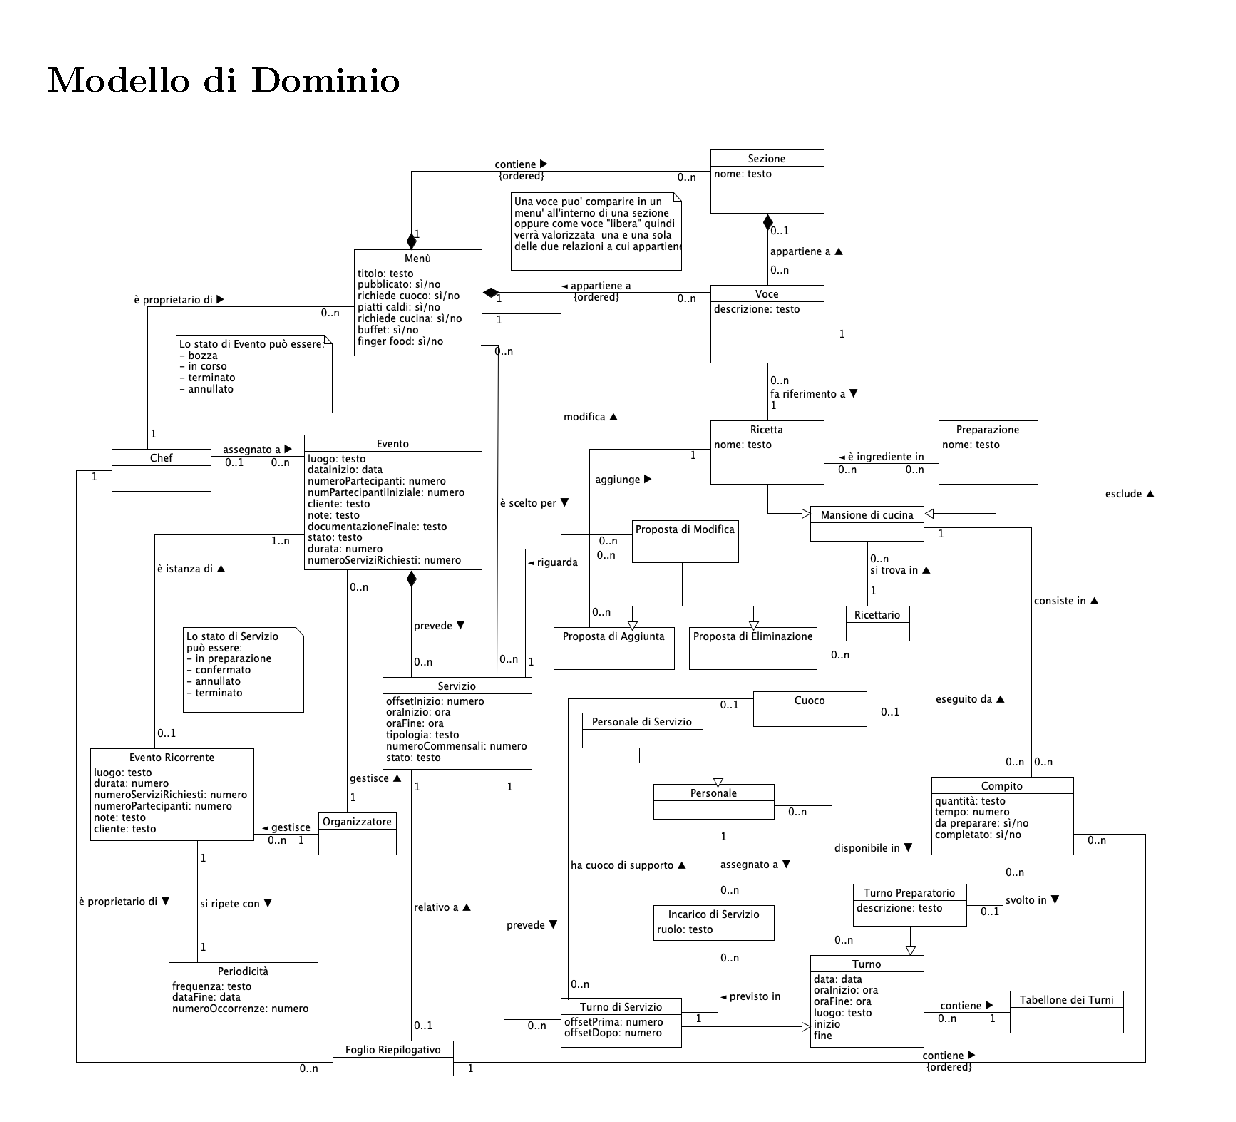
\includepdf[pages=-, fitpaper=true, pagecommand={\thispagestyle{empty}}]{img/domain_model/domain_model_titled.pdf}


\chapter{Diagrammi di Sequenza di Sistema (SSD)}

\section{Scenario Principale}
\label{sec:ssd_main}

\begin{figure}[H]
  \centering
  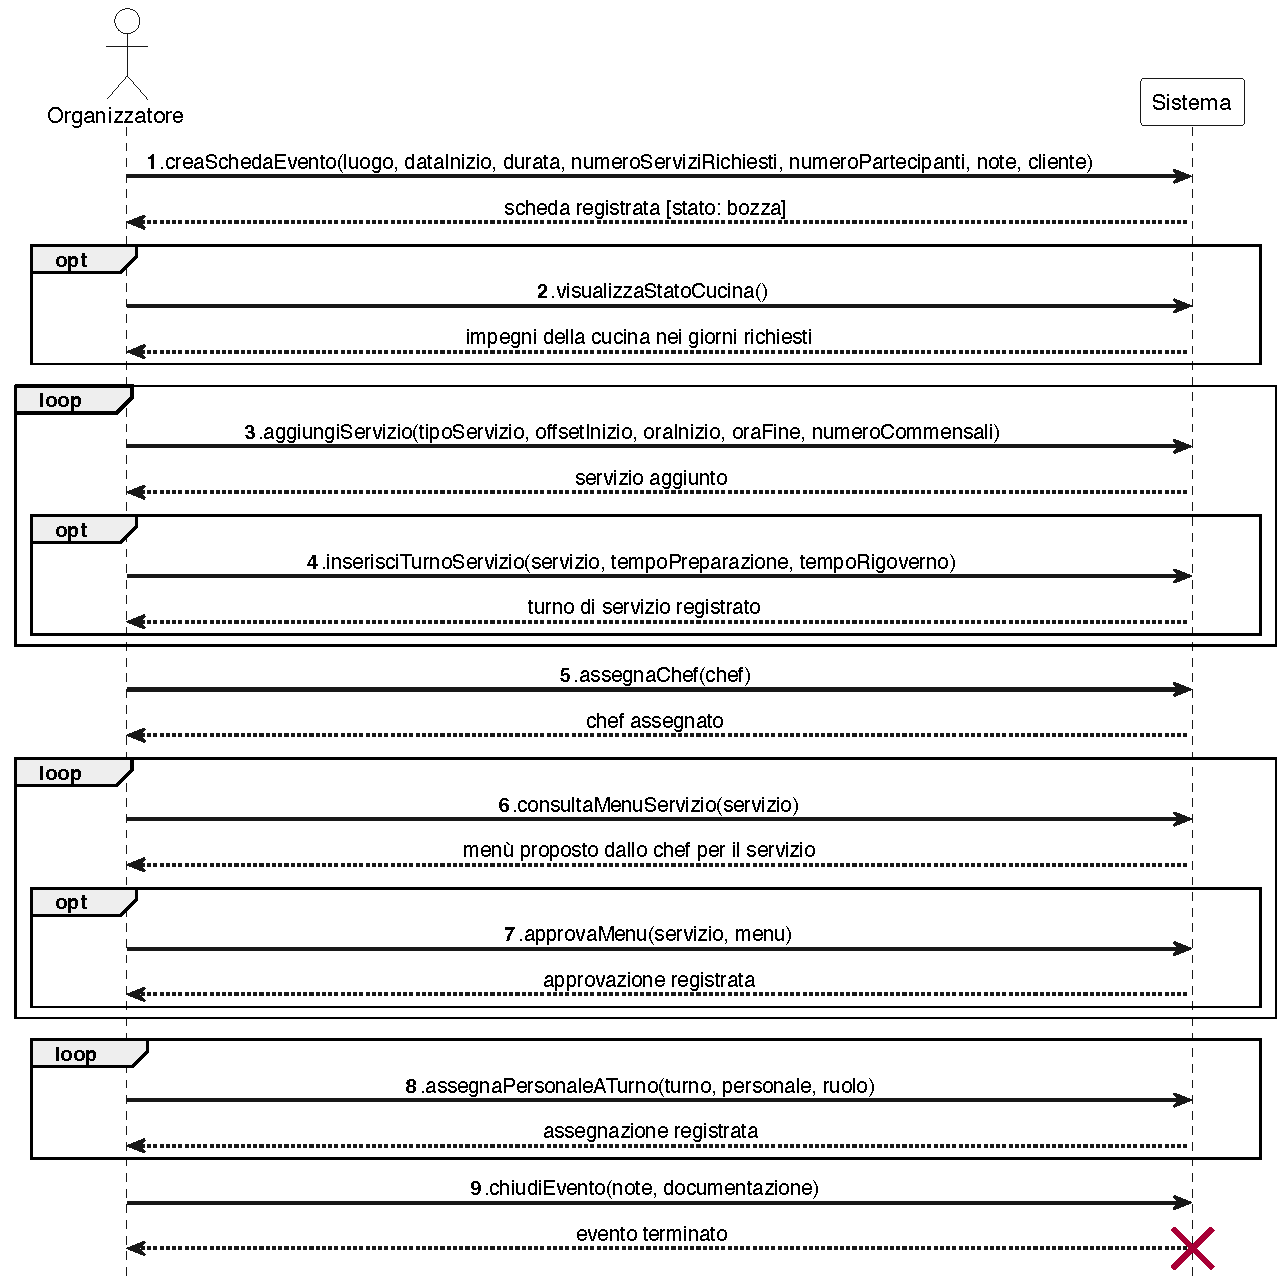
\includegraphics[width=\textwidth]{ssd/ssd_main}
\end{figure}

\newgeometry{margin=1cm}

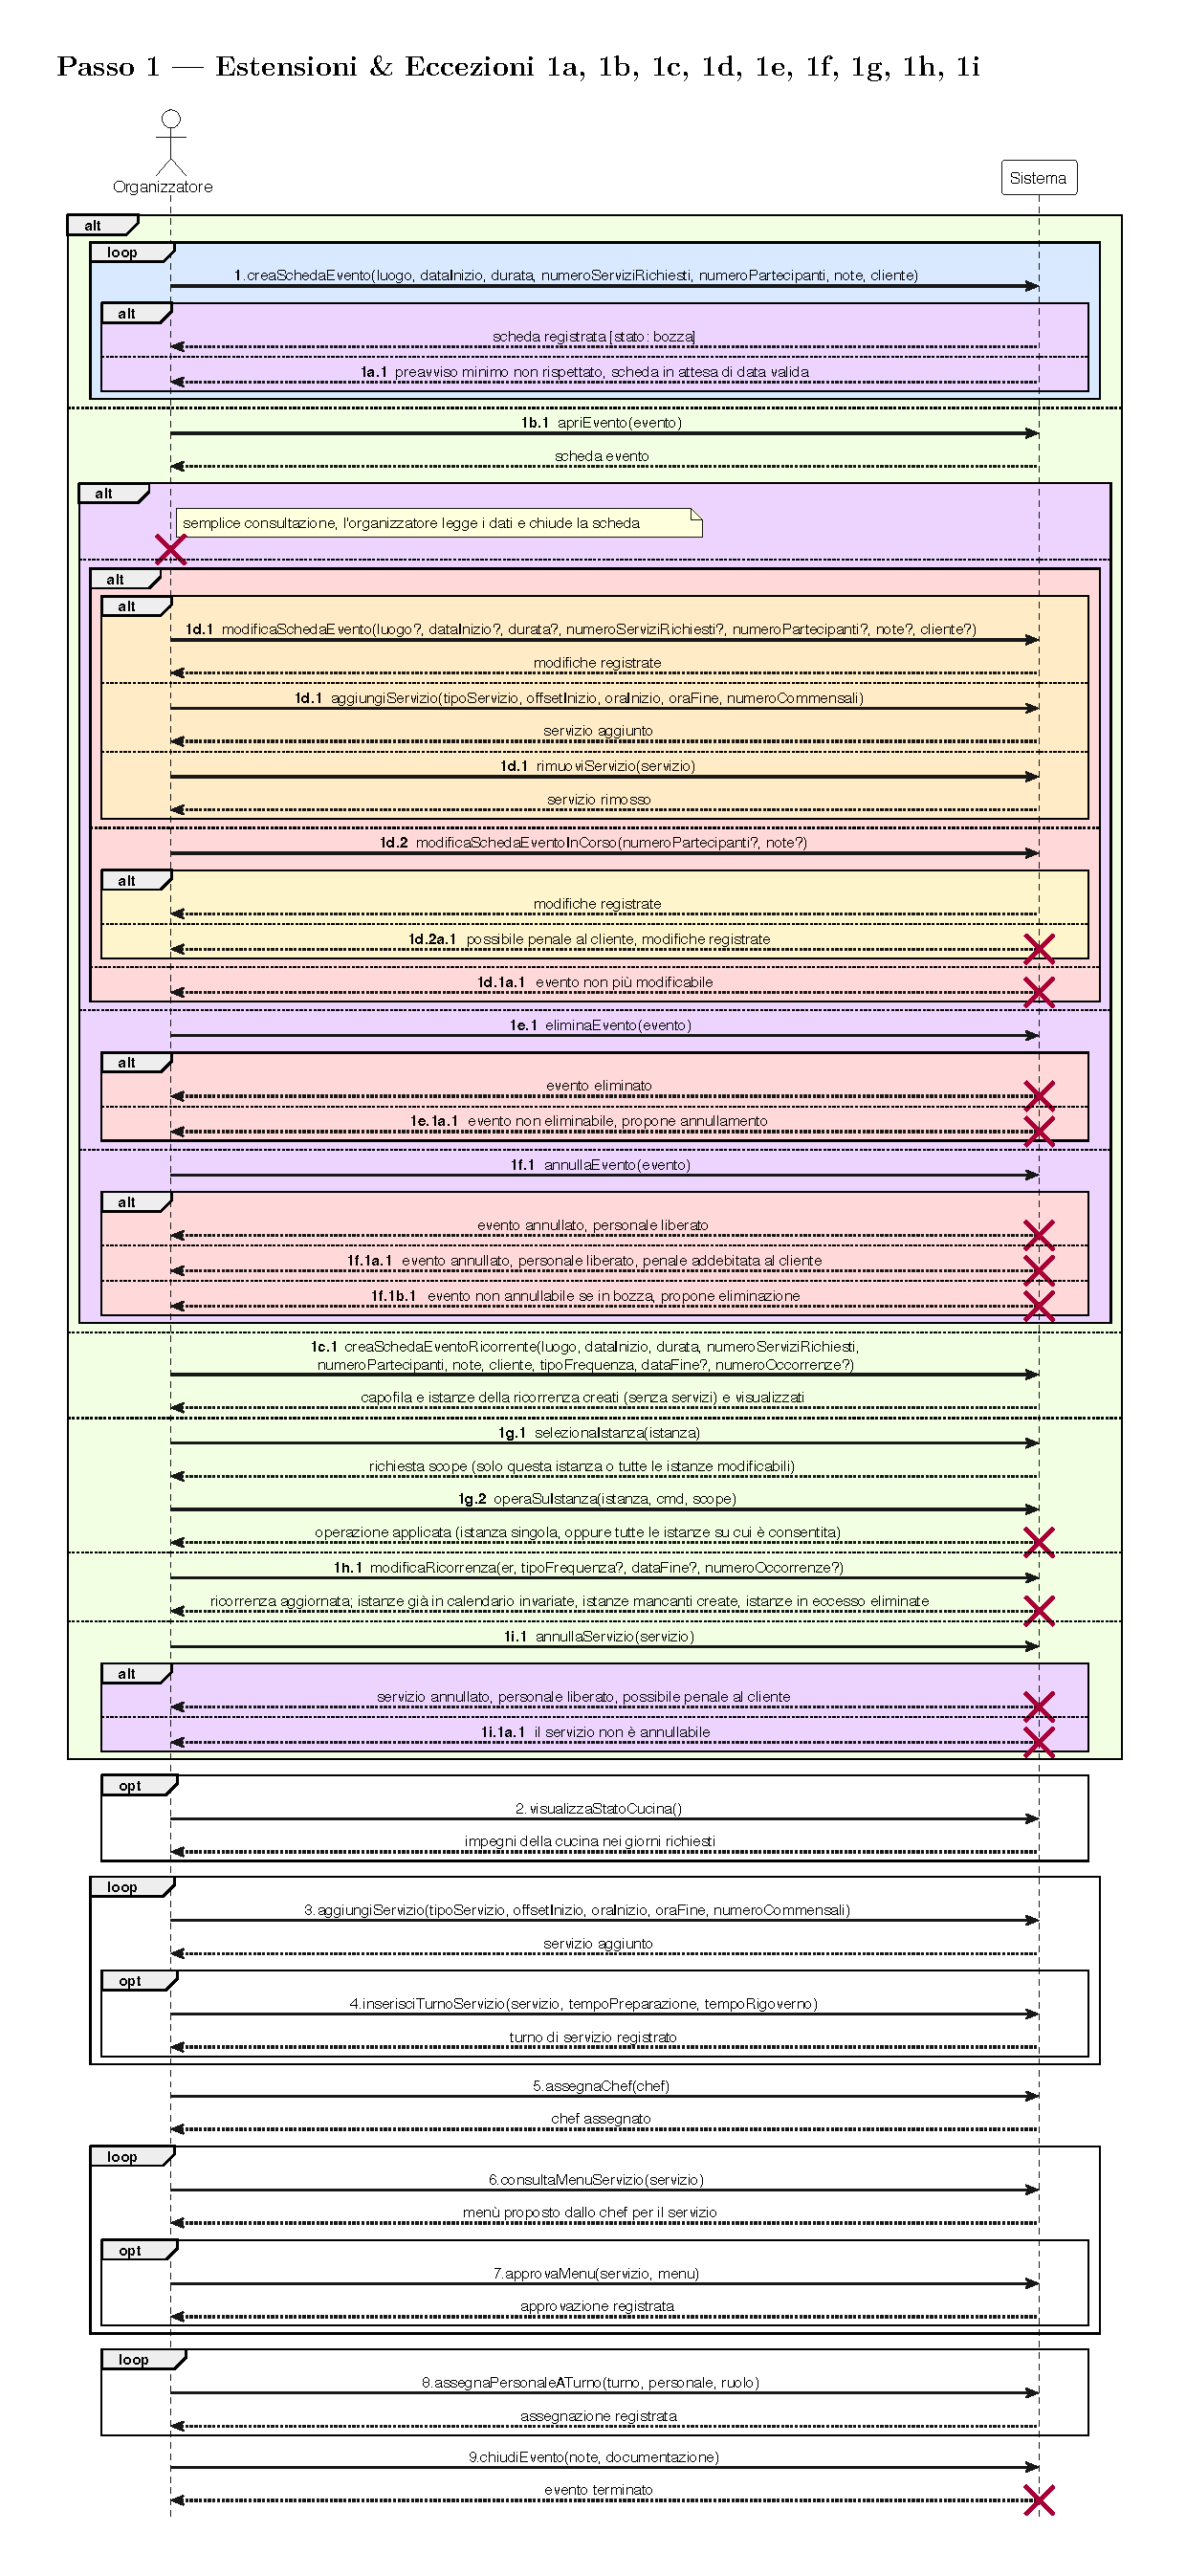
\includepdf[pages=-, fitpaper=true, pagecommand={\thispagestyle{empty}}]{img/ssd/ssd_ext1_titled.pdf}

% ─────────────────────────────────────────────────────────────
\newpage
\section{Passi 2, 3, 4 --- Estensioni \& Eccezioni 3a}
\label{sec:ssd_ext3}

\begin{figure}[H]
  \centering
  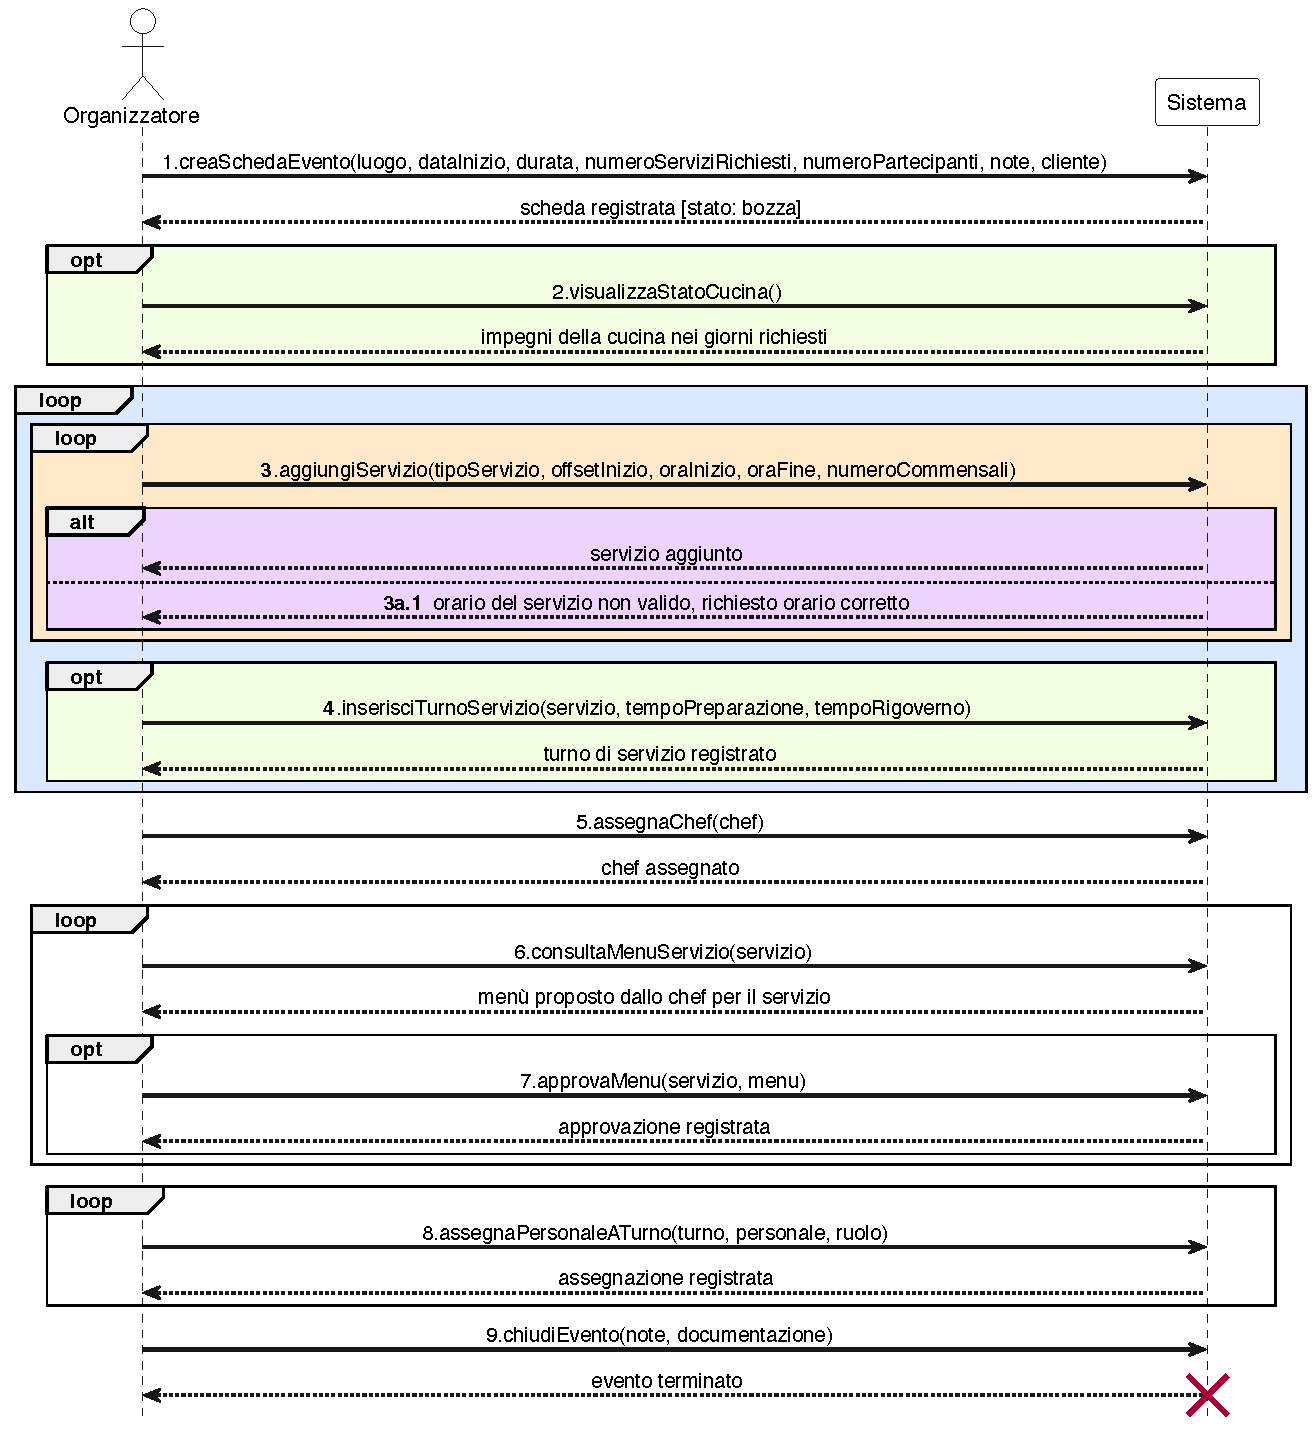
\includegraphics[width=\textwidth, height=0.85\textheight, keepaspectratio]{ssd/ssd_ext3}
\end{figure}

% ─────────────────────────────────────────────────────────────
\newpage
\section{Passo 5 --- Estensioni \& Eccezioni 5a, 5b}
\label{sec:ssd_ext5}

\begin{figure}[H]
  \centering
  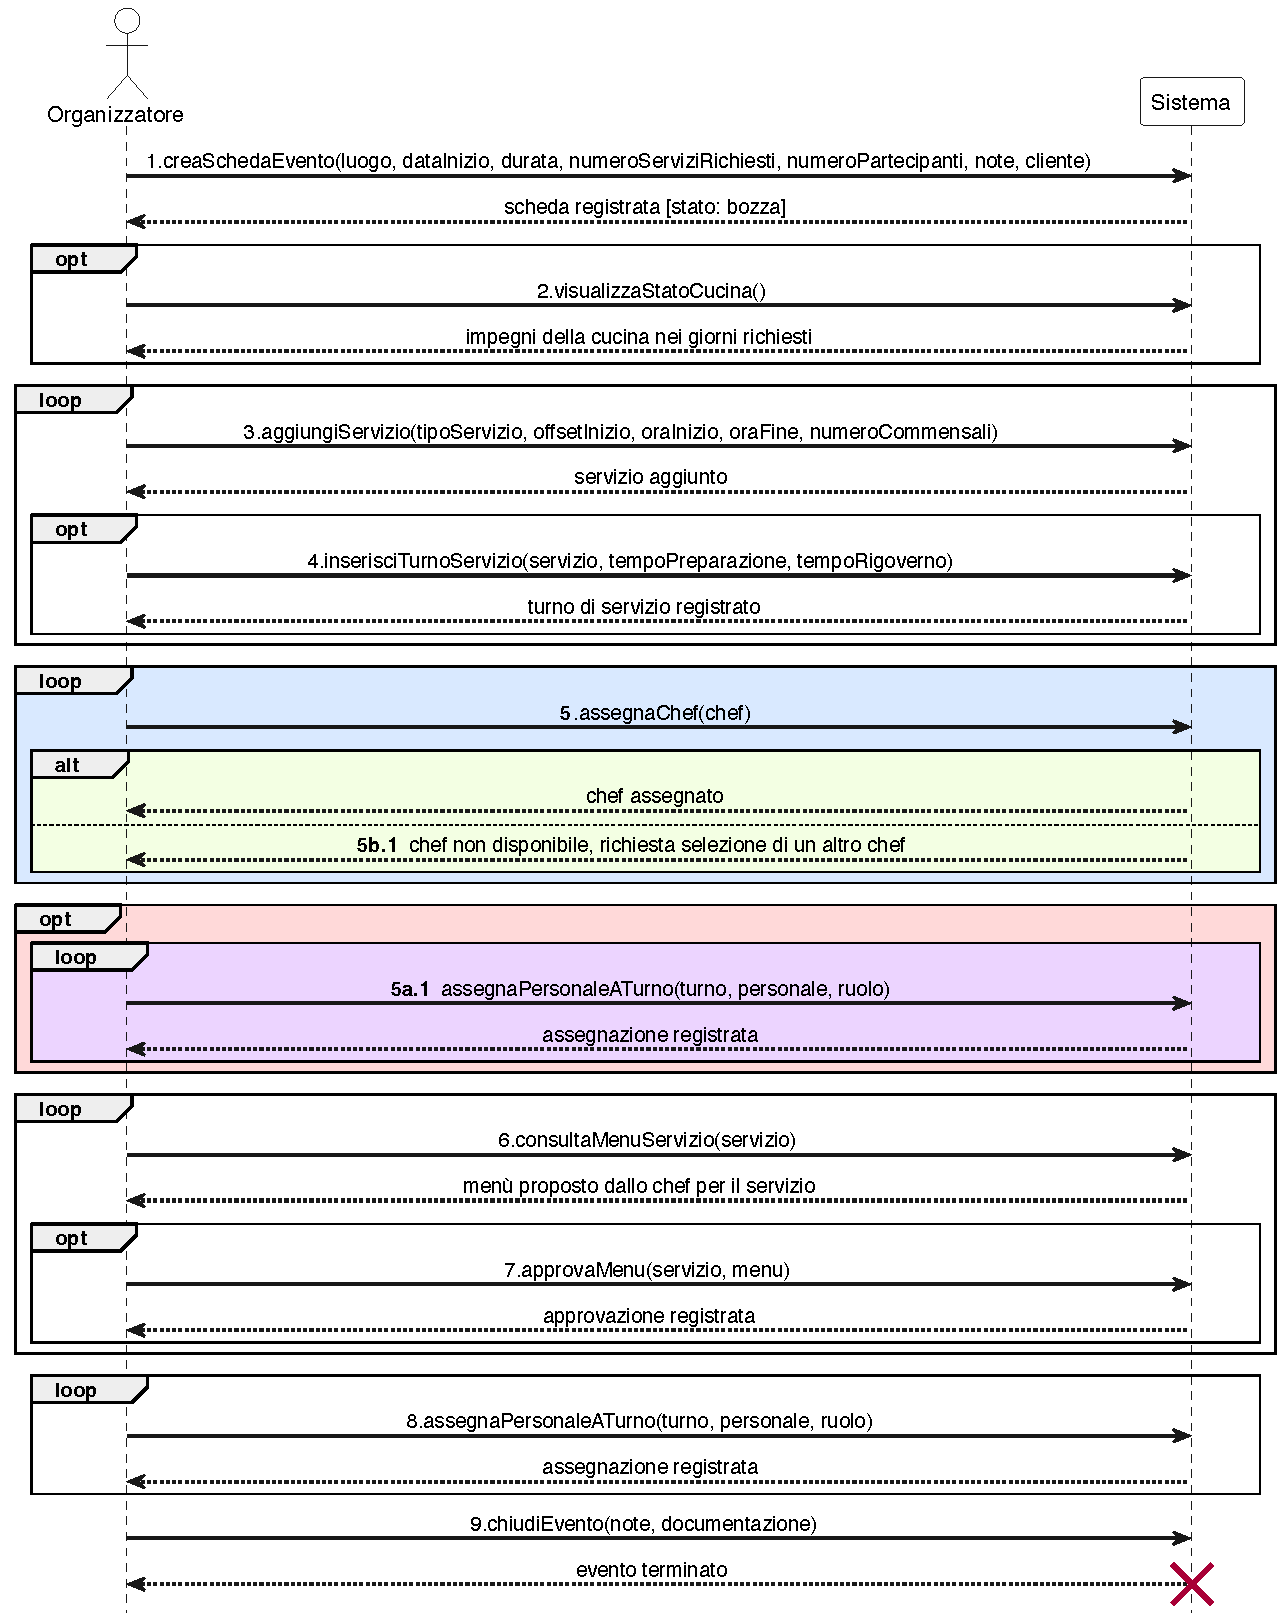
\includegraphics[width=\textwidth, height=0.85\textheight, keepaspectratio]{ssd/ssd_ext5}
\end{figure}

% ─────────────────────────────────────────────────────────────
\newpage
\section{Passi 6, 7 --- Estensioni \& Eccezioni 7a, 7b}
\label{sec:ssd_ext6}

\begin{figure}[H]
  \centering
  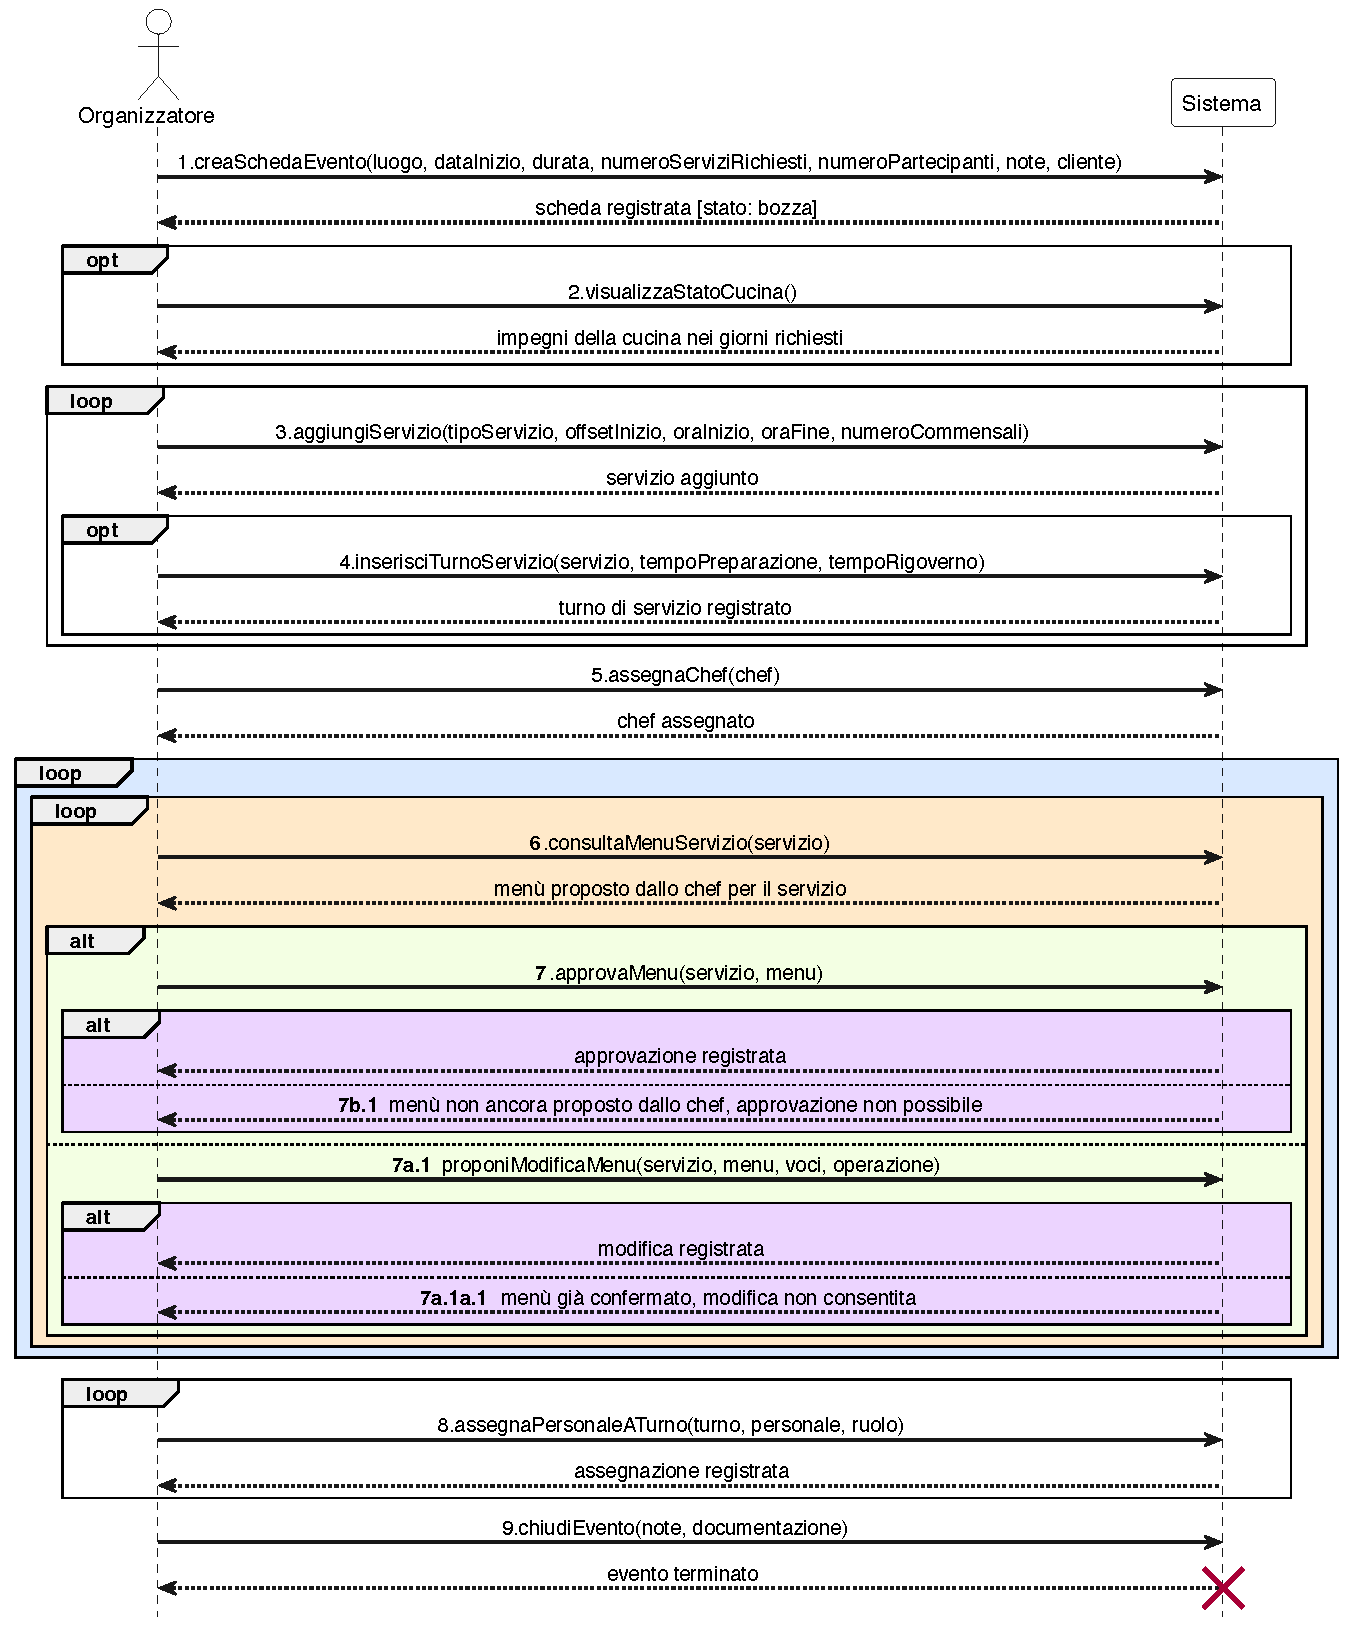
\includegraphics[width=\textwidth, height=0.85\textheight, keepaspectratio]{ssd/ssd_ext6}
\end{figure}

% ─────────────────────────────────────────────────────────────
\newpage
\section{Passo 8 --- Estensioni \& Eccezioni 8a, 8b, 8c}
\label{sec:ssd_ext7}

\begin{figure}[H]
  \centering
  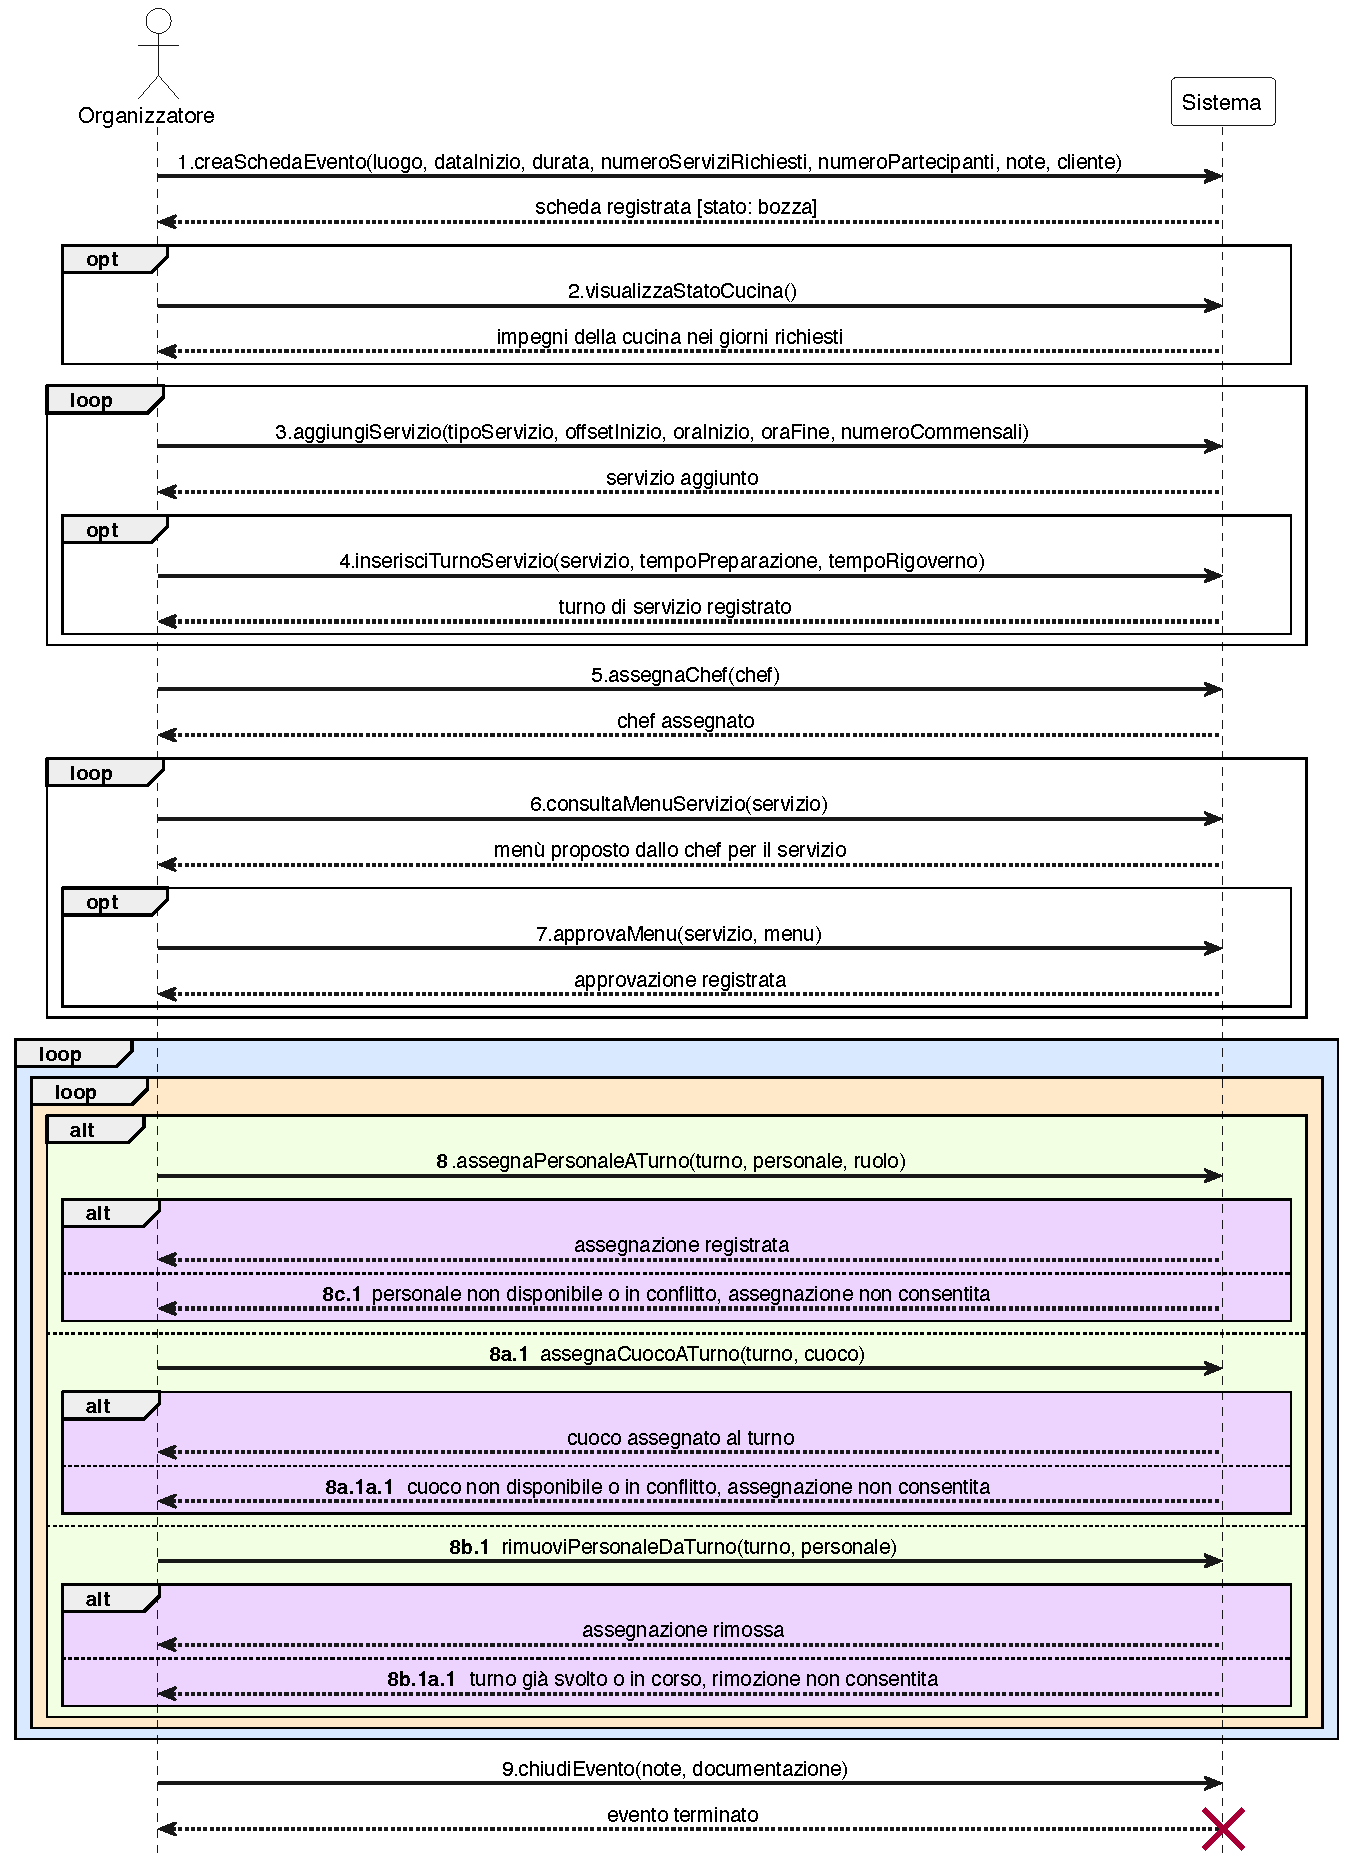
\includegraphics[width=\textwidth, height=0.82\textheight, keepaspectratio]{ssd/ssd_ext7}
\end{figure}

% ─────────────────────────────────────────────────────────────
\newpage
\section{Passo 9 --- Estensioni \& Eccezioni 9a}
\label{sec:ssd_ext8}

\begin{figure}[H]
  \centering
  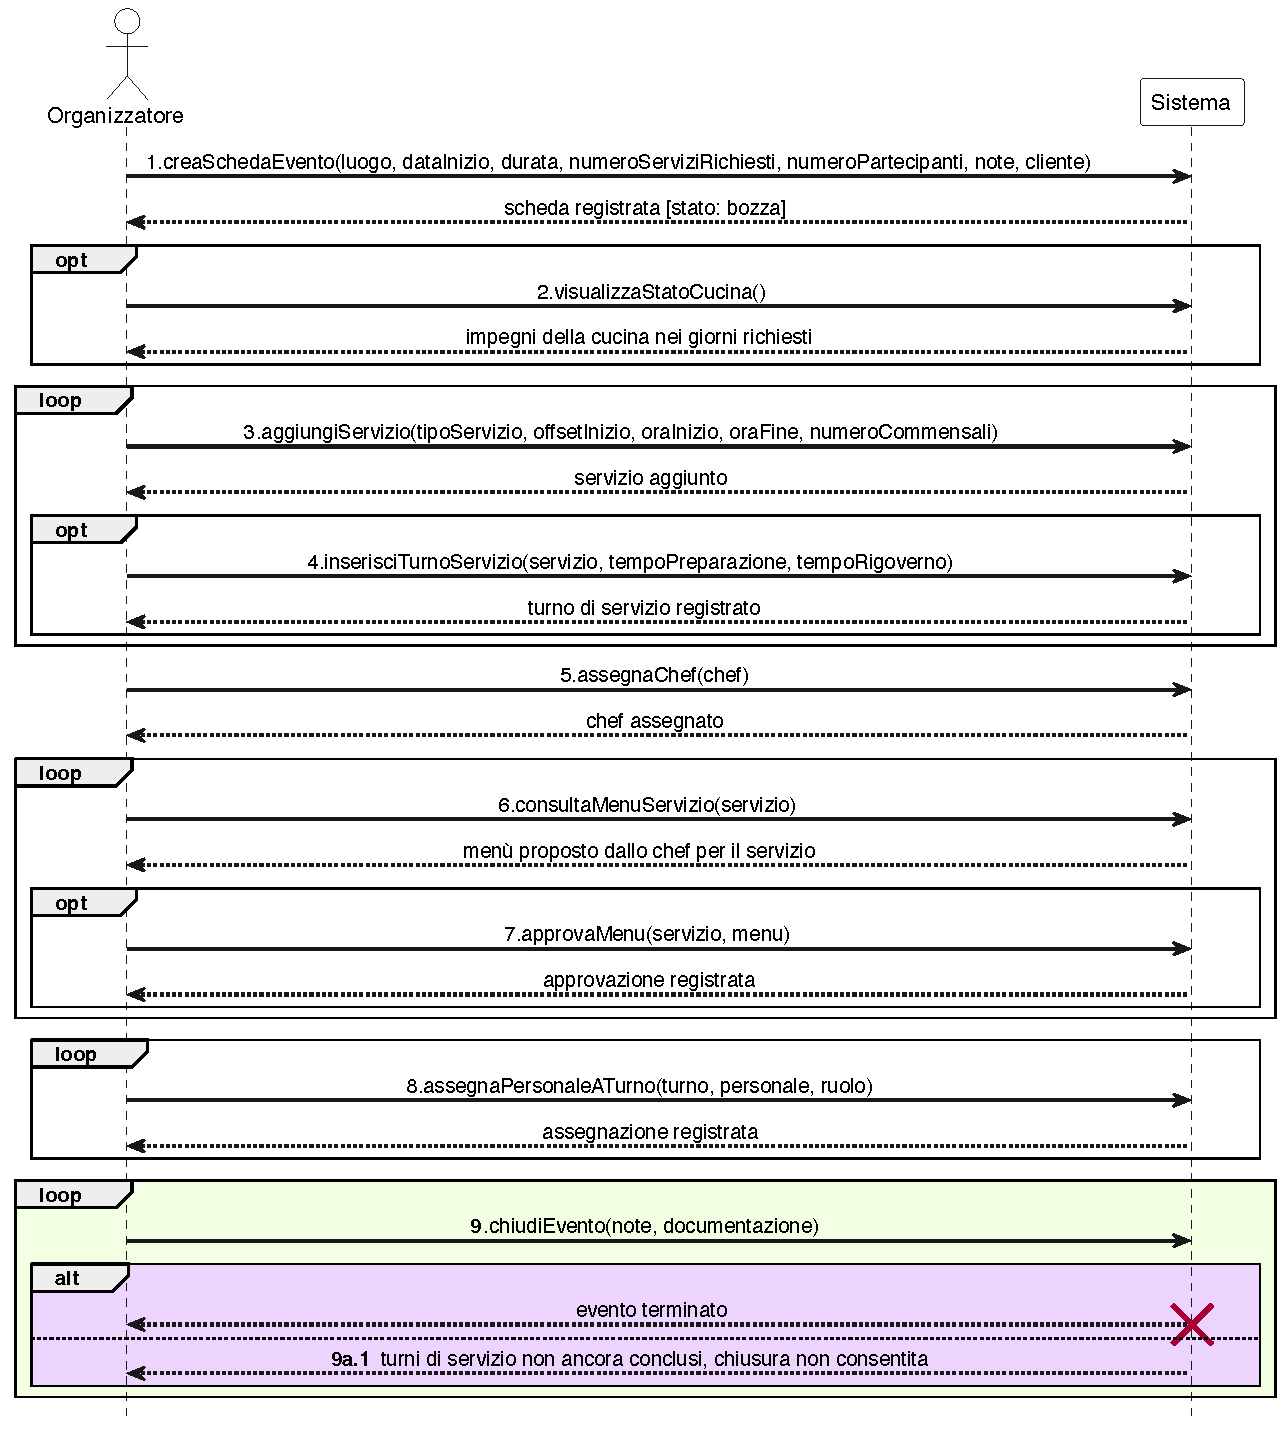
\includegraphics[width=\textwidth, height=0.85\textheight, keepaspectratio]{ssd/ssd_ext8}
\end{figure}

\restoregeometry
\newpage


\chapter{Contratti delle Operazioni}
% ─────────────────────────────────────────────────────────────
%  Contratti delle Operazioni — Gestire gli eventi
%  Ordinati per passo/estensione del caso d'uso: 1, 1a, 1b, ...,
%  2, 3, 4, 5, 5a, 5b, 6, 7, 7a, 8, 8a, 8b, 9.
%
%  Convenzioni tipografiche (vedi \cobj/\cparam/\crel in main.tex):
%    corsivo         istanza/oggetto già legato (es. e, me, org)
%    sottolineato     parametro formale dell'operazione, ovunque citato
%    grassetto        relazione/ruolo/verbo logico del modello di dominio
%    testo normale    nomi di classe e valori letterali di stato
% ─────────────────────────────────────────────────────────────

\noindent\textbf{Pre-condizione generale:} l'attore è identificato con
un'istanza \cobj{org} di Organizzatore.

\bigskip

% ─── 1. creaSchedaEvento ─────────────────────────────────────
\begin{contratto}{1. creaSchedaEvento(\cparam{luogo}: String, \cparam{dataInizio}: LocalDate, \cparam{durata}: int, \cparam{numeroServiziRichiesti}: int, \cparam{numeroPartecipanti}: int, \cparam{note}: String, \cparam{cliente}: String)}
  \cpre{%
    La data corrente dista da \cparam{dataInizio} almeno due
    settimane (soglia maggiore, a discrezione dell'organizzatore,
    per eventi di grandi dimensioni --- 50 o più partecipanti ---
    o che si estendono su più giornate); altrimenti Eccezione 1a.1.
  }
  \cpost{%
    \mbox{}\par
    \begin{itemize}[nosep]
      \item È stata creata un'istanza \cobj{e} di Evento,
            senza ancora alcun Servizio associato.
      \item \cobj{e.luogo} = \cparam{luogo};
      \item \cobj{e.dataInizio} = \cparam{dataInizio};
      \item \cobj{e.durata} = \cparam{durata};
      \item \cobj{e.numeroServiziRichiesti} = \cparam{numeroServiziRichiesti}.
      \item \cobj{e.note} = \cparam{note};
      \item \cobj{e.cliente} = \cparam{cliente}.
      \item \cobj{e.numeroPartecipanti} = \cparam{numeroPartecipanti}.
      \item \cobj{e.numPartecipantiIniziale} = \cparam{numeroPartecipanti}.
      \item \cobj{e.stato} = bozza.
      \item \cobj{org} \crel{gestisce} \cobj{e}.
    \end{itemize}
  }
\end{contratto}

% ─── 1b.1. apriEvento ────────────────────────────────────────
\begin{contratto}{1b.1 apriEvento(\cparam{evento}: Event)}
  \cpre{%
    \mbox{}\par
    \begin{itemize}[nosep]
      \item \cparam{evento}.stato = bozza oppure
            \cparam{evento}.stato = in\_corso oppure
            \cparam{evento}.stato = terminato oppure
            \cparam{evento}.stato = annullato.
      \item \cobj{org} \crel{gestisce} \cparam{evento}.
    \end{itemize}
  }
  \cpost{(nessuna --- navigazione alla scheda evento esistente)}
\end{contratto}

% ─── 1c.1. creaSchedaEventoRicorrente ───────────────────────
\newpage
\begin{contratto}{1c.1 creaSchedaEventoRicorrente(\cparam{luogo}: String, \cparam{dataInizio}: LocalDate, \cparam{durata}: int, \cparam{numeroServiziRichiesti}: int, \cparam{numeroPartecipanti}: int, \cparam{note}: String, \cparam{cliente}: String, \cparam{tipoFrequenza}: String, \cparam{dataFine}?: LocalDate, \cparam{numeroOccorrenze}?: Integer)}
  \cpre{%
    \mbox{}\par
    \begin{itemize}[nosep]
      \item La data corrente dista dalla data di inizio della prima istanza almeno due settimane (soglia
            maggiore, a discrezione dell'organizzatore, per eventi di grandi dimensioni --- 50 o più
            partecipanti --- o che si estendono su più giornate); altrimenti Eccezione 1a.
      \item[\textit{Nota:}] \cparam{dataFine} e \cparam{numeroOccorrenze} sono alternativi tra loro: ne
            va specificato esattamente uno.
    \end{itemize}
  }
  \cpost{%
    \mbox{}\par
    \begin{itemize}[nosep]
      \item È stata creata un'istanza \cobj{me} di Evento Ricorrente, con
            \cobj{me.luogo} = \cparam{luogo}, \cobj{me.durata} = \cparam{durata},
            \cobj{me.numeroServiziRichiesti} = \cparam{numeroServiziRichiesti},
            \cobj{me.numeroPartecipanti} = \cparam{numeroPartecipanti},
            \cobj{me.note} = \cparam{note}, \cobj{me.cliente} = \cparam{cliente}.
      \item È stata creata un'istanza \cobj{p} di Periodicità
            con \cobj{p.frequenza} = \cparam{tipoFrequenza},
            \cobj{p.dataFine} = \cparam{dataFine} oppure \cobj{p.numeroOccorrenze}
            = \cparam{numeroOccorrenze} (a seconda di quale dei due è stato specificato);
            \cobj{me} \crel{si ripete con} \cobj{p}.
      \item Per ogni data calcolata dalla frequenza fino alla
            conclusione: è stata creata un'istanza \cobj{e} di
            Evento, senza ancora alcun Servizio
            associato; \cobj{e} è \crel{istanza di} \cobj{me};
            \cobj{e} eredita \cparam{luogo}, \cparam{durata},
            \cparam{numeroServiziRichiesti}, \cparam{numeroPartecipanti},
            \cparam{note}, \cparam{cliente} dal capofila; \cobj{e.dataInizio} è
            calcolata secondo \cobj{p}; \cobj{e.stato} = bozza.
      \item \cobj{e.numPartecipantiIniziale} = \cparam{numeroPartecipanti}.
      \item \cobj{org} \crel{gestisce} \cobj{me}.
      \vspace{\baselineskip}
      \item[\textit{Nota:}] i servizi aggiunti (mediante
            aggiungiServizio) a una qualunque istanza ancora in
            stato bozza, finché la serie è in fase di costruzione,
            vengono replicati automaticamente sulle altre istanze
            ancora in stato bozza della stessa ricorrenza.
    \end{itemize}
  }
\end{contratto}

% ─── 1d.1. modificaSchedaEvento ─────────────────────────────
\begin{contratto}{1d.1 modificaSchedaEvento(\cparam{luogo}?: String, \cparam{dataInizio}?: LocalDate, \cparam{durata}?: Integer, \cparam{numeroServiziRichiesti}?: Integer, \cparam{numeroPartecipanti}?: Integer, \cparam{note}?: String, \cparam{cliente}?: String)}
  \cpre{%
    È in corso la gestione di un Evento \cobj{e} in stato
    bozza; altrimenti Eccezione 1d.1a.
  }
  \cpost{%
    \mbox{}\par
    \begin{itemize}[nosep]
      \item Per ogni parametro descrittivo fornito
            (\cparam{luogo}, \cparam{dataInizio}, \cparam{durata},\\
            \cparam{numeroServiziRichiesti}, \cparam{numeroPartecipanti},
            \cparam{note}, \cparam{cliente}), il corrispondente
            attributo di \cobj{e} è stato aggiornato.
      \item Se \cparam{numeroPartecipanti} è specificato:
            \cobj{e.numPartecipantiIniziale} = \cparam{numeroPartecipanti}
            (il valore iniziale di riferimento per il controllo di
            variazione resta così allineato all'ultimo valore
            confermato prima dell'avvio dei lavori).
    \end{itemize}
  }
\end{contratto}

\smallskip
\noindent\textit{Nota:} l'aggiunta di un servizio a un evento in bozza
riusa i contratti \textbf{3. aggiungiServizio} e
\textbf{4. inserisciTurnoServizio}; la rimozione usa il contratto
dedicato seguente.
\smallskip

% ─── 1d.1. rimuoviServizio ───────────────────────────────────
\newpage
\begin{contratto}{1d.1 (rimozione servizio) rimuoviServizio(\cparam{servizio}: Service)}
  \cpre{%
    \mbox{}\par
    \begin{itemize}[nosep]
      \item È in corso la gestione di un Evento \cobj{e} in stato
            bozza; altrimenti Eccezione 1d.1a.
      \item \cparam{servizio} è un Servizio di \cobj{e}.
    \end{itemize}
  }
  \cpost{%
    \mbox{}\par
    \begin{itemize}[nosep]
      \item Il Turno di Servizio associato a \cparam{servizio} e
            ogni Incarico di Servizio in esso previsto sono stati
            eliminati.
      \item \cparam{servizio} è stato eliminato da \cobj{e}.
    \end{itemize}
  }
\end{contratto}

% ─── 1d.2. modificaSchedaEventoInCorso ──────────────────────
\begin{contratto}{1d.2 modificaSchedaEventoInCorso(\cparam{numeroPartecipanti}?: Integer, \cparam{note}?: String)}
  \cpre{%
    È in corso la gestione di un Evento \cobj{e} in stato
    in\_corso; altrimenti Eccezione 1d.1a.
  }
  \cpost{%
    \mbox{}\par
    \begin{itemize}[nosep]
      \item Se \cparam{numeroPartecipanti} è specificato:
            \cobj{e.numeroPartecipanti} = \cparam{numeroPartecipanti}.
      \item Se \cparam{note} è specificato: \cobj{e.note} =
            \cparam{note}.
      \item Se \cparam{numeroPartecipanti} è specificato con una
            variazione superiore al 30\% rispetto al valore
            iniziale: il sistema segnala che potrebbe essere
            addebitata una penale al cliente (Eccezione 1d.2a),
            lasciando l'eventuale deroga a discrezione
            dell'organizzatore.
    \end{itemize}
  }
\end{contratto}

% ─── 1e.1. eliminaEvento ─────────────────────────────────────
\begin{contratto}{1e.1 eliminaEvento(\cparam{evento}: Event)}
  \cpre{%
    \mbox{}\par
    \begin{itemize}[nosep]
      \item \cobj{org} \crel{gestisce} \cparam{evento}.
      \item \cparam{evento}.stato = bozza; altrimenti Eccezione 1e.1a.
    \end{itemize}
  }
  \cpost{%
    \mbox{}\par
    \begin{itemize}[nosep]
      \item Per ogni Servizio associato a \cparam{evento}: il Turno di
            Servizio associato e ogni Incarico di Servizio in esso
            previsto sono stati eliminati, e il Servizio stesso è stato
            eliminato.
      \item \cparam{evento} è stato eliminato.
    \end{itemize}
  }
\end{contratto}

% ─── 1f.1. annullaEvento ─────────────────────────────────────
\begin{contratto}{1f.1 annullaEvento(\cparam{evento}: Event)}
  \cpre{%
    \mbox{}\par
    \begin{itemize}[nosep]
      \item \cobj{org} \crel{gestisce} \cparam{evento}.
      \item \cparam{evento}.stato = in\_corso; altrimenti Eccezione 1f.1b.
    \end{itemize}
  }
  \cpost{%
    \mbox{}\par
    \begin{itemize}[nosep]
      \item \cparam{evento}.stato = annullato.
      \item Per ogni Servizio \cobj{s} in cui \cparam{evento} è
            suddiviso: \cobj{s.stato} = annullato e ogni Incarico
            di Servizio previsto in un Turno di servizio di
            \cobj{s} è stato eliminato.
      \item Se la data corrente è a meno di una settimana da
            \cparam{evento}.dataInizio: il sistema segnala che verrà
            addebitata una penale al cliente (Eccezione 1f.1a).
    \end{itemize}
  }
\end{contratto}

% ─── 1g.1. selezionaIstanza ───────────────────────────────────
\newpage
\begin{contratto}{1g.1 selezionaIstanza(\cparam{istanza}: Event)}
  \cpre{%
    \mbox{}\par
    \begin{itemize}[nosep]
      \item \cparam{istanza} è \crel{istanza di} un Evento Ricorrente \cobj{er}.
      \item \cobj{org} \crel{gestisce} \cobj{er}.
    \end{itemize}
  }
  \cpost{(nessuna --- navigazione all'istanza selezionata, in vista
    della richiesta dello scope dell'operazione successiva)}
\end{contratto}

% ─── 1g.2. operaSuIstanza ────────────────────────────────────
\begin{contratto}{1g.2 operaSuIstanza(\cparam{istanza}: Event, \cparam{cmd}: EventCommand, \cparam{scope}: Scope)}
  \cpre{%
    \mbox{}\par
    \begin{itemize}[nosep]
      \item \cparam{istanza} è \crel{istanza di} un Evento Ricorrente \cobj{er}
            (\cparam{istanza} è un Evento).
      \item \cobj{org} \crel{gestisce} \cobj{er}.
      \item[\textit{Nota:}] \cparam{cmd} è un'operazione già selezionata
            e predisposta dall'attore (modifica, annullamento o
            eliminazione) da eseguire su una o più istanze; il tipo
            concreto di \cparam{cmd} determina quale delle tre
            operazioni viene applicata.
    \end{itemize}
  }
  \cpost{%
    \mbox{}\par
    \begin{itemize}[nosep]
      \item Se \cparam{scope} = SINGOLA: \cparam{cmd} è \crel{stata
            applicata a} \cparam{istanza}, se le regole di
            modificabilità lo consentono (\cparam{istanza} non deve
            trovarsi in stato terminato né annullato); altrimenti
            l'operazione non ha effetto su \cparam{istanza}.
      \item Se \cparam{scope} = TUTTE: \cparam{cmd} è \crel{stata
            applicata a} ogni Evento \crel{istanza di} \cobj{er}
            su cui era consentita (cioè non in stato terminato né
            annullato).
    \end{itemize}
  }
\end{contratto}

% ─── 1h.1. modificaRicorrenza ────────────────────────────────
\begin{contratto}{1h.1 modificaRicorrenza(\cparam{er}: RecurringEvent, \cparam{tipoFrequenza}?: String, \cparam{dataFine}?: LocalDate, \cparam{numeroOccorrenze}?: Integer)}
  \cpre{%
    \mbox{}\par
    \begin{itemize}[nosep]
      \item \cparam{er} è un Evento Ricorrente che \crel{si ripete
            con} una Periodicità \cobj{p}.
      \item \cobj{org} \crel{gestisce} \cparam{er}.
      \item Esiste almeno un Evento \crel{istanza di} \cparam{er}
            non ancora annullato né terminato.
    \end{itemize}
  }
  \cpost{%
    \mbox{}\par
    \begin{itemize}[nosep]
      \item Se \cparam{tipoFrequenza} è specificata: \cobj{p.frequenza} = \cparam{tipoFrequenza}.
      \item Se \cparam{dataFine} è specificata: \cobj{p.dataFine} = \cparam{dataFine}.
      \item Se \cparam{numeroOccorrenze} è specificato:
            \cobj{p.numeroOccorrenze} = \cparam{numeroOccorrenze}.
      \vspace{\baselineskip}
      \item[\textit{Nota:}] \cparam{dataFine} e \cparam{numeroOccorrenze}
            sono alternativi tra loro: ne va specificato al più uno.
      \vspace{\baselineskip}
      \item Le istanze già presenti in calendario sono rimaste invariate.
      \item Le istanze in eccesso (fuori dalla nuova conclusione) sono
            state eliminate.
      \item Le istanze mancanti (generate dalla nuova frequenza o
            conclusione) sono state create sul modello del capofila
            \cparam{er}.
    \end{itemize}
  }
\end{contratto}

% ─── 1i.1. annullaServizio ───────────────────────────────────
\newpage
\begin{contratto}{1i.1 annullaServizio(\cparam{servizio}: Service)}
  \cpre{%
    \mbox{}\par
    \begin{itemize}[nosep]
      \item È in corso la gestione di un Evento \cobj{e}.
      \item \cparam{servizio} è un Servizio di \cobj{e}.
      \item \cparam{servizio}.stato $\neq$ annullato e
            \cparam{servizio}.stato $\neq$ terminato; altrimenti
            Eccezione 1i.1a.
    \end{itemize}
  }
  \cpost{%
    \mbox{}\par
    \begin{itemize}[nosep]
      \item \cparam{servizio}.stato = annullato.
      \item Ogni Incarico di Servizio previsto in un
            Turno di servizio di \cparam{servizio} è stato
            eliminato.
      \item Il sistema segnala la possibilità di una penale al
            cliente.
    \end{itemize}
  }
\end{contratto}

% ─── 2. visualizzaStatoCucina ─────────────────────────────────
\begin{contratto}{2. visualizzaStatoCucina()}
  \cpre{È in corso la gestione di un Evento \cobj{e}.}
  \cpost{(nessuna --- interrogazione al sistema)}
\end{contratto}

% ─── 3. aggiungiServizio ──────────────────────────────────────
\begin{contratto}{3. aggiungiServizio(\cparam{tipoServizio}: String, \cparam{offsetInizio}: int, \cparam{oraInizio}: LocalTime, \cparam{oraFine}: LocalTime, \cparam{numeroCommensali}: int)}
  \cpre{%
    \mbox{}\par
    \begin{itemize}[nosep]
      \item È in corso la gestione di un Evento \cobj{e} in stato
            bozza.
      \item La data del servizio, calcolata da \cobj{e.dataInizio} e
            \cparam{offsetInizio}, non precede la data corrente e resta
            entro l'intervallo di date previsto per \cobj{e};
            altrimenti Eccezione 3a.
    \end{itemize}
  }
  \cpost{%
    \mbox{}\par
    \begin{itemize}[nosep]
      \item È stata creata un'istanza \cobj{s} di Servizio.
      \item \cobj{s.tipologia} = \cparam{tipoServizio};
      \item \cobj{s.offsetInizio} = \cparam{offsetInizio};
      \item \cobj{s.oraInizio} = \cparam{oraInizio};
      \item \cobj{s.oraFine} = \cparam{oraFine};
      \item \cobj{s.numeroCommensali} = \cparam{numeroCommensali};
      \item \cobj{s.stato} = in\_preparazione;
      \item \cobj{e} \crel{prevede} \cobj{s}.
      \item Se \cobj{e} è istanza di un Evento ricorrente, un Servizio
            con gli stessi attributi è stato creato in ogni altra
            istanza ancora in stato bozza per cui la data risultante è
            valida.
    \end{itemize}
  }
\end{contratto}

% ─── 4. inserisciTurnoServizio ───────────────────────────────
\newpage
\begin{contratto}{4. inserisciTurnoServizio(\cparam{servizio}: Service, \cparam{tempoPreparazione}: int, \cparam{tempoRigoverno}: int)}
  \cpre{%
    \mbox{}\par
    \begin{itemize}[nosep]
      \item È in corso la gestione di un Evento \cobj{e} in stato
            bozza.
      \item \cparam{servizio} è un Servizio di \cobj{e}.
    \end{itemize}
  }
  \cpost{%
    \mbox{}\par
    \begin{itemize}[nosep]
      \item È stata creata un'istanza \cobj{t} di Turno di servizio;
      \item \cobj{t.offsetPrima} = \cparam{tempoPreparazione};
      \item \cobj{t.offsetDopo} = \cparam{tempoRigoverno};
      \item \cobj{t.luogo} = \cobj{e.luogo};
      \item detti \cobj{i} e \cobj{f} l'istante di inizio e quello di fine di
            \cparam{servizio} --- ricavati dalla data del servizio, calcolata
            da \cobj{e.dataInizio} e \cparam{servizio}.offsetInizio, e dalle
            ore \cparam{servizio}.oraInizio e \cparam{servizio}.oraFine ---
            si ha \cobj{t.inizio} = \cobj{i} anticipato di
            \cparam{tempoPreparazione} e \cobj{t.fine} = \cobj{f} posticipato
            di \cparam{tempoRigoverno};
      \item se \cparam{servizio}.oraFine non è successiva a
            \cparam{servizio}.oraInizio, il servizio attraversa la mezzanotte
            e \cobj{f} cade nel giorno seguente; vale comunque
            \cobj{t.inizio} $<$ \cobj{t.fine};
      \item \cparam{servizio} \crel{prevede} \cobj{t}.
    \end{itemize}
  }
\end{contratto}

% ─── 5. assegnaChef ──────────────────────────────────────────
\begin{contratto}{5. assegnaChef(\cparam{chef}: User)}
  \cpre{%
    \mbox{}\par
    \begin{itemize}[nosep]
      \item È in corso la gestione di un Evento \cobj{e} in stato bozza.
      \item \cparam{chef} ha effettivamente il ruolo di Chef.
      \item Lo chef indicato è disponibile e non ha altri incarichi in
            conflitto nelle date dell'evento; altrimenti Eccezione 5b.
    \end{itemize}
  }
  \cpost{%
    \mbox{}\par
    \begin{itemize}[nosep]
      \item \cobj{e} è \crel{assegnato a} \cparam{chef}.
    \end{itemize}
  }
\end{contratto}

% ─── 6. consultaMenuServizio ─────────────────────────────────
\begin{contratto}{6. consultaMenuServizio(\cparam{servizio}: Service)}
  \cpre{%
    \mbox{}\par
    \begin{itemize}[nosep]
      \item È in corso la gestione di un Evento \cobj{e}.
      \item \cparam{servizio} è un Servizio di \cobj{e}.
    \end{itemize}
  }
  \cpost{(nessuna --- interrogazione al sistema: restituisce il
    Menù scelto per \cparam{servizio})}
\end{contratto}

% ─── 7. approvaMenu ──────────────────────────────────────────
\begin{contratto}{7. approvaMenu(\cparam{servizio}: Service, \cparam{menu}: Menu)}
  \cpre{%
    \mbox{}\par
    \begin{itemize}[nosep]
      \item È in corso la gestione di un Evento \cobj{e} in stato
            bozza.
      \item \cparam{servizio} è un Servizio di \cobj{e}.
      \item \cparam{menu} è stato proposto dallo chef ed è scelto per
            \cparam{servizio}, con \cparam{servizio}.stato =
            in\_preparazione; altrimenti (nessun menù ancora
            proposto) Eccezione 7b.
    \end{itemize}
  }
  \cpost{%
    \mbox{}\par
    \begin{itemize}[nosep]
      \item \cparam{servizio}.stato = confermato (lo stato del
            Servizio a cui \cparam{menu} è associato segnala
            l'approvazione).
      \item Se tutti i Servizi di \cobj{e} sono in stato
            confermato: \cobj{e.stato} = in\_corso.
    \end{itemize}
  }
\end{contratto}

% ─── 7a.1. proponiModificaMenu ────────────────────────────────
\begin{contratto}{7a.1 proponiModificaMenu(\cparam{servizio}: Service, \cparam{menu}: Menu, \cparam{voci}: List$\langle$MenuItem$\rangle$, \cparam{operazione}: ProposalOperation)}
  \cpre{%
    \mbox{}\par
    \begin{itemize}[nosep]
      \item È in corso la gestione di un Evento \cobj{e}.
      \item \cparam{servizio} è un Servizio di \cobj{e} con
            \cparam{servizio}.stato = in\_preparazione; altrimenti
            (menù già confermato) Eccezione 7a.1a.
      \item \cparam{menu} è scelto per \cparam{servizio}.
    \end{itemize}
  }
  \cpost{%
    \mbox{}\par
    \begin{itemize}[nosep]
      \item È stata creata un'istanza \cobj{pm} di
            Proposta di Modifica, nella specifica sottoclasse
            Proposta di Aggiunta o Proposta di
            Eliminazione secondo \cparam{operazione}.
      \item \cobj{pm} \crel{riguarda} \cparam{servizio}.
      \item \cobj{pm} \crel{modifica} \cparam{menu}.
      \item Il Menù originale non è modificato.
    \end{itemize}
  }
\end{contratto}

% ─── 8. assegnaPersonaleATurno ───────────────────────────────
\begin{contratto}{8. assegnaPersonaleATurno(\cparam{turno}: ServiceShift, \cparam{personale}: User, \cparam{ruolo}: String)}
  \cpre{%
    \mbox{}\par
    \begin{itemize}[nosep]
      \item È in corso la gestione di un Evento \cobj{e}.
      \item \cparam{turno} è un Turno di servizio previsto da un
            Servizio di \cobj{e}.
      \item \cparam{personale} ha il ruolo di Personale di servizio.
      \item Il membro del personale inserito ha fornito la propria
            disponibilità per la fascia oraria del turno e non ha
            incarichi concomitanti in altre sedi; altrimenti Eccezione 8c.
    \end{itemize}
  }
  \cpost{%
    \mbox{}\par
    \begin{itemize}[nosep]
      \item È stata creata un'istanza \cobj{a} di
            Incarico di Servizio.
      \item \cobj{a.ruolo} = \cparam{ruolo}.
      \item \cobj{a} è \crel{assegnato a} \cparam{personale}.
      \item \cobj{a} è \crel{previsto in} \cparam{turno}.
      \vspace{\baselineskip}
      \item[\textit{Nota:}] l'operazione può essere eseguita anche in
            via anticipata, come previsto dall'Estensione 5a del caso
            d'uso, prima dell'approvazione definitiva dei menù dei
            servizi; l'assegnazione resta valida
            indipendentemente dallo stato di approvazione del menù.
    \end{itemize}
  }
\end{contratto}

% ─── 8a.1. assegnaCuocoATurno ────────────────────────────────
\begin{contratto}{8a.1 assegnaCuocoATurno(\cparam{turno}: ServiceShift, \cparam{cuoco}: User)}
  \cpre{%
    \mbox{}\par
    \begin{itemize}[nosep]
      \item È in corso la gestione di un Evento \cobj{e}.
      \item \cparam{turno} è un Turno di servizio previsto da un
            Servizio di \cobj{e}.
      \item \cparam{cuoco} ha il ruolo di Cuoco.
      \item Il cuoco indicato ha fornito la propria disponibilità per
            la fascia oraria del turno e non ha incarichi concomitanti
            in altre sedi; altrimenti Eccezione 8a.1a.
    \end{itemize}
  }
  \cpost{%
    \mbox{}\par
    \begin{itemize}[nosep]
      \item \cparam{turno} \crel{ha cuoco di supporto} \cparam{cuoco}.
      \vspace{\baselineskip}
      \item[\textit{Nota:}] a differenza dell'assegnazione del
            personale di servizio (contratto 8), il cuoco di supporto
            non genera un Incarico di Servizio: un Turno di servizio
            ha al più un cuoco di supporto, assegnato direttamente.
    \end{itemize}
  }
\end{contratto}

% ─── 8b.1. rimuoviPersonaleDaTurno ───────────────────────────
\begin{contratto}{8b.1 rimuoviPersonaleDaTurno(\cparam{turno}: ServiceShift, \cparam{personale}: User)}
  \cpre{%
    \mbox{}\par
    \begin{itemize}[nosep]
      \item È in corso la gestione di un Evento \cobj{e}.
      \item Esiste un Incarico di Servizio assegnato a
            \cparam{personale} e previsto in \cparam{turno}.
      \item \cparam{turno} è ancora modificabile (non ancora svolto,
            né in corso di svolgimento); altrimenti Eccezione 8b.1a.
    \end{itemize}
  }
  \cpost{%
    \mbox{}\par
    \begin{itemize}[nosep]
      \item L'istanza di Incarico di Servizio assegnata a
            \cparam{personale} e prevista in \cparam{turno} è stata
            eliminata.
    \end{itemize}
  }
\end{contratto}

% ─── 9. chiudiEvento ─────────────────────────────────────────
\begin{contratto}{9. chiudiEvento(\cparam{note}: String, \cparam{documentazione}: String)}
  \cpre{%
    \mbox{}\par
    \begin{itemize}[nosep]
      \item \cobj{e.stato} = in\_corso.
      \item Tutti i turni di servizio previsti da \cobj{e} sono
            conclusi (data/ora già passata); altrimenti Eccezione 9a.
    \end{itemize}
  }
  \cpost{%
    \mbox{}\par
    \begin{itemize}[nosep]
      \item \cobj{e.stato} = terminato.
      \item Ogni Servizio \cobj{s} di \cobj{e} è stato impostato
            allo stato terminato.
      \item \cobj{e.note} viene aggiornato accodando \cparam{note}.
      \item \cobj{e.documentazioneFinale} = \cparam{documentazione}.
    \end{itemize}
  }
\end{contratto}


% Titolo capitolo e diagramma sono disegnati insieme dentro
% img/dcd/dcd_titled.pdf (rigenerato con `python3 build_dcd_titled.py`
% dopo un eventuale aggiornamento manuale di img/dcd/dcd.png), su una
% pagina dimensionata su misura attorno al contenuto -- niente pagina
% A4 landscape fissa che lasciava spazio vuoto sopra/sotto quando
% l'aspect ratio del diagramma non corrispondeva a quello della pagina.
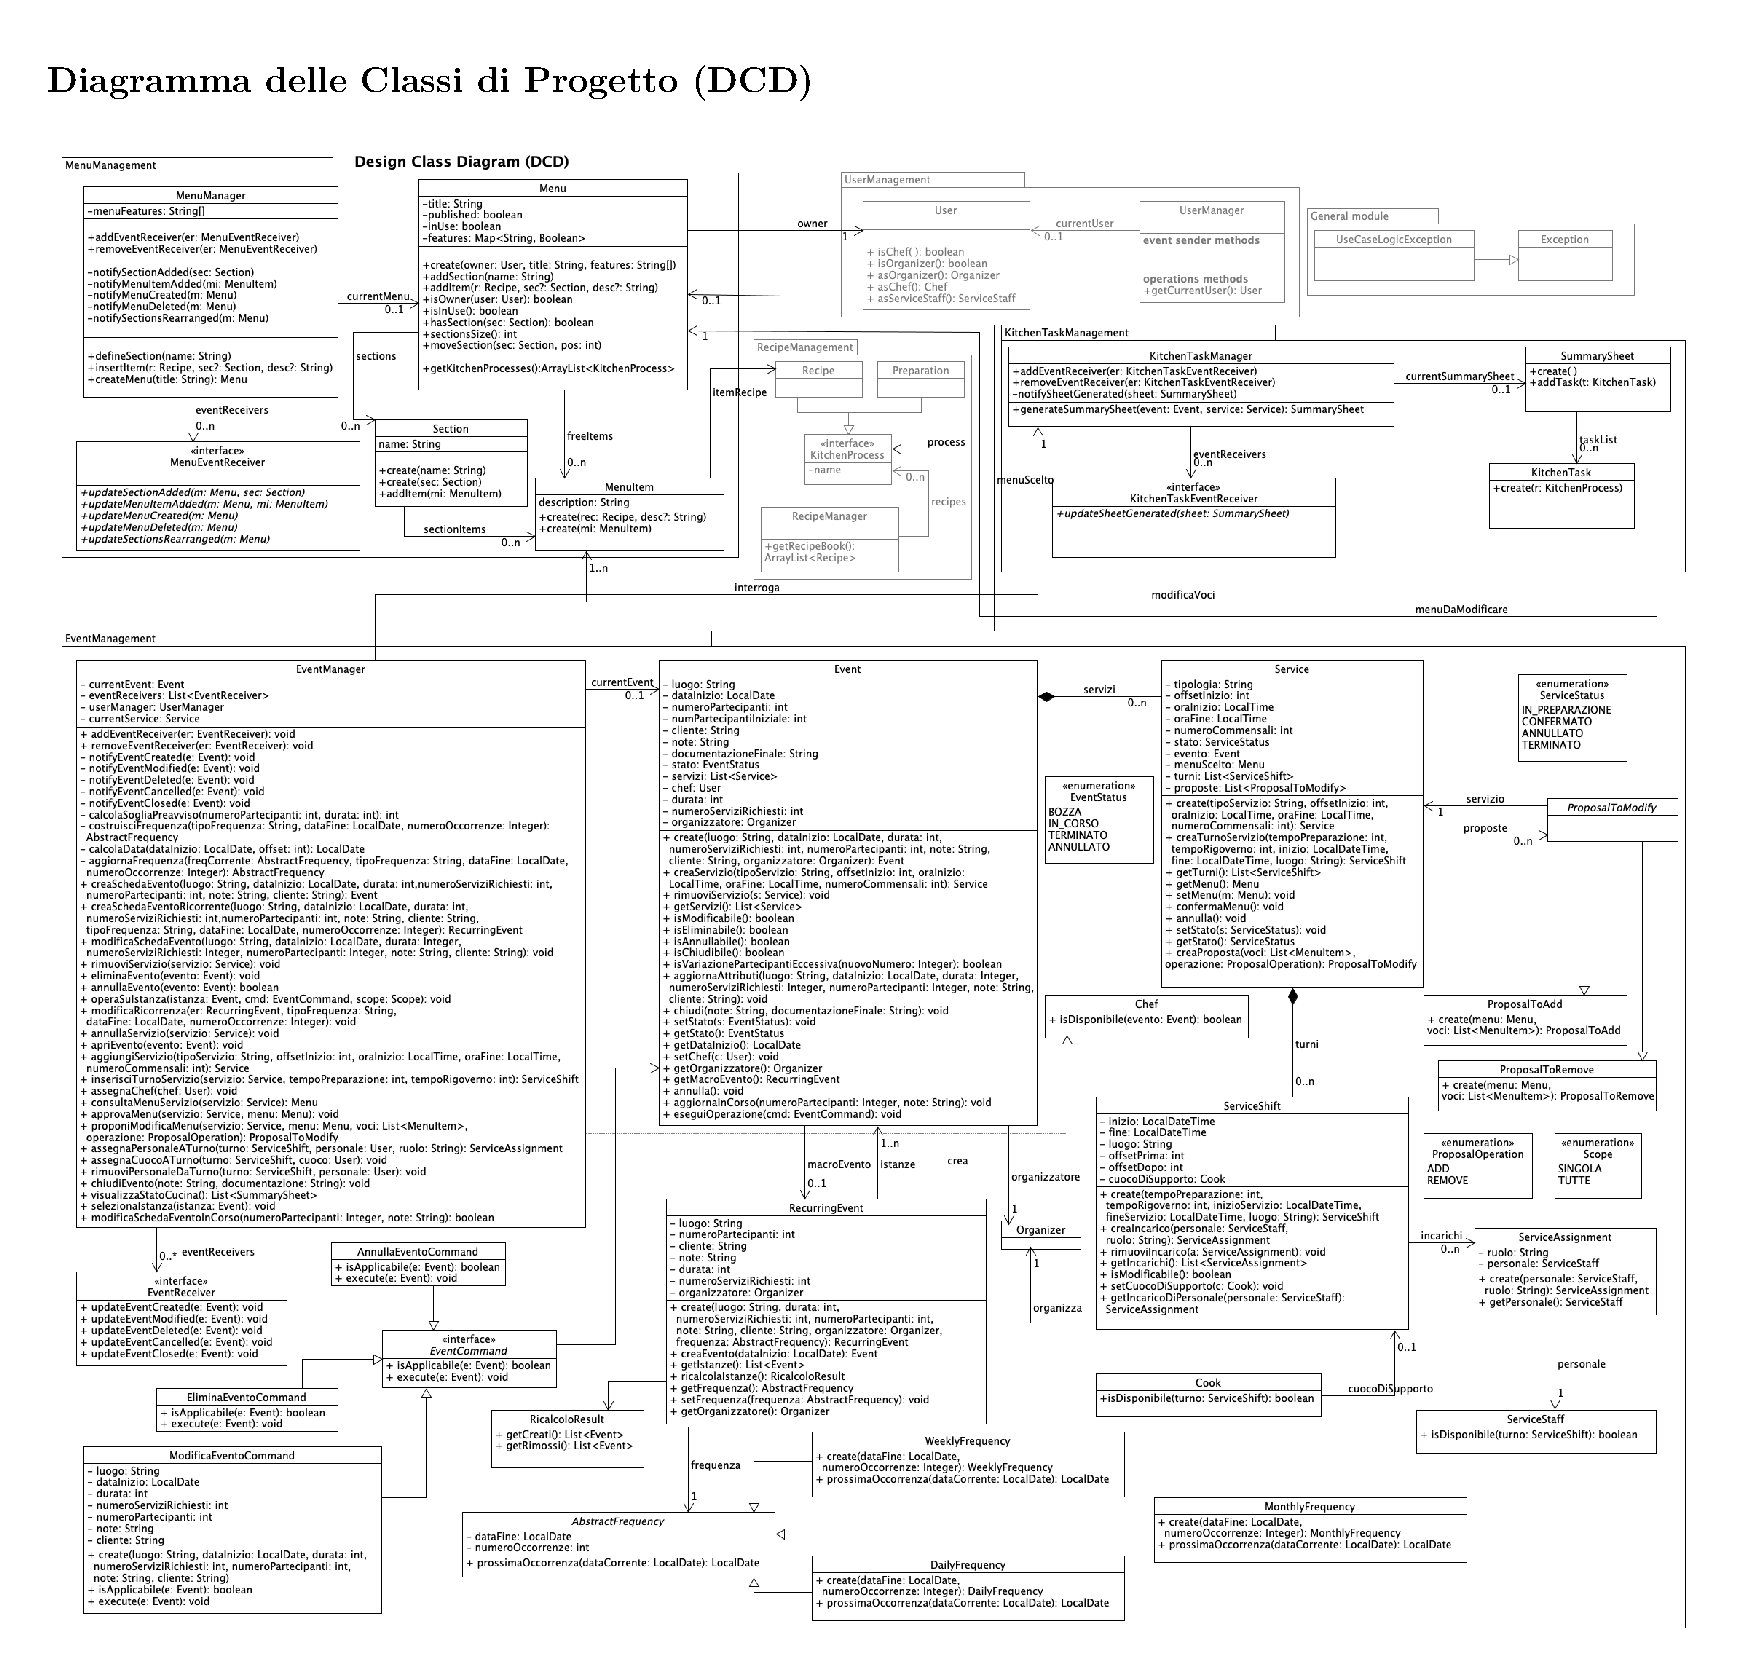
\includepdf[pages=-, fitpaper=true, pagecommand={\thispagestyle{empty}}]{img/dcd/dcd_titled.pdf}

% Titolo capitolo e primo diagramma (op1) condividono la stessa pagina
% orizzontale (vedi capitoli/dsd.tex) -- niente \chapter{} qui, che
% forzerebbe una pagina portrait a sé stante solo per il titolo, dato
% che sia \chapter sia \begin{landscape} interrompono comunque pagina
% per conto proprio. Il contatore di capitolo avanza comunque.

\newcommand{\dsdpage}[1]{%
  \pdfpagewidth=841.89pt
  \pdfpageheight=#1pt
  \hoffset=-35.59pt
  \voffset=-35.59pt
  \textwidth=796.53pt
  \hsize=796.53pt
  \textheight=#1pt
  \addtolength{\textheight}{-45.36pt}
  \vsize=\textheight
  \marginparwidth=0pt
}

\newcommand{\dsdrestorepage}{%
  \pdfpagewidth=595.276pt
  \pdfpageheight=841.89pt
  \hoffset=-21.25pt
  \voffset=-21.25pt
  \textwidth=493.23pt
  \hsize=493.23pt
  \textheight=739.84pt
  \vsize=\textheight
  \marginparwidth=35pt
}

\newlength{\dsdscreenw}
\newlength{\dsdscreenh}
\newlength{\dsdscreenhfirst}
\setlength{\dsdscreenw}{781pt}
\setlength{\dsdscreenh}{476pt}
\setlength{\dsdscreenhfirst}{401pt}

\clearpage
\dsdpage{595.276}

{\LARGE\bfseries Diagrammi di Sequenza Dettagliati (DSD)\par}
\vspace{0.8em}

\section{op1 --- \texttt{creaSchedaEvento}}
\label{sec:dsd_op1}

\begin{figure}[H]
  \centering
  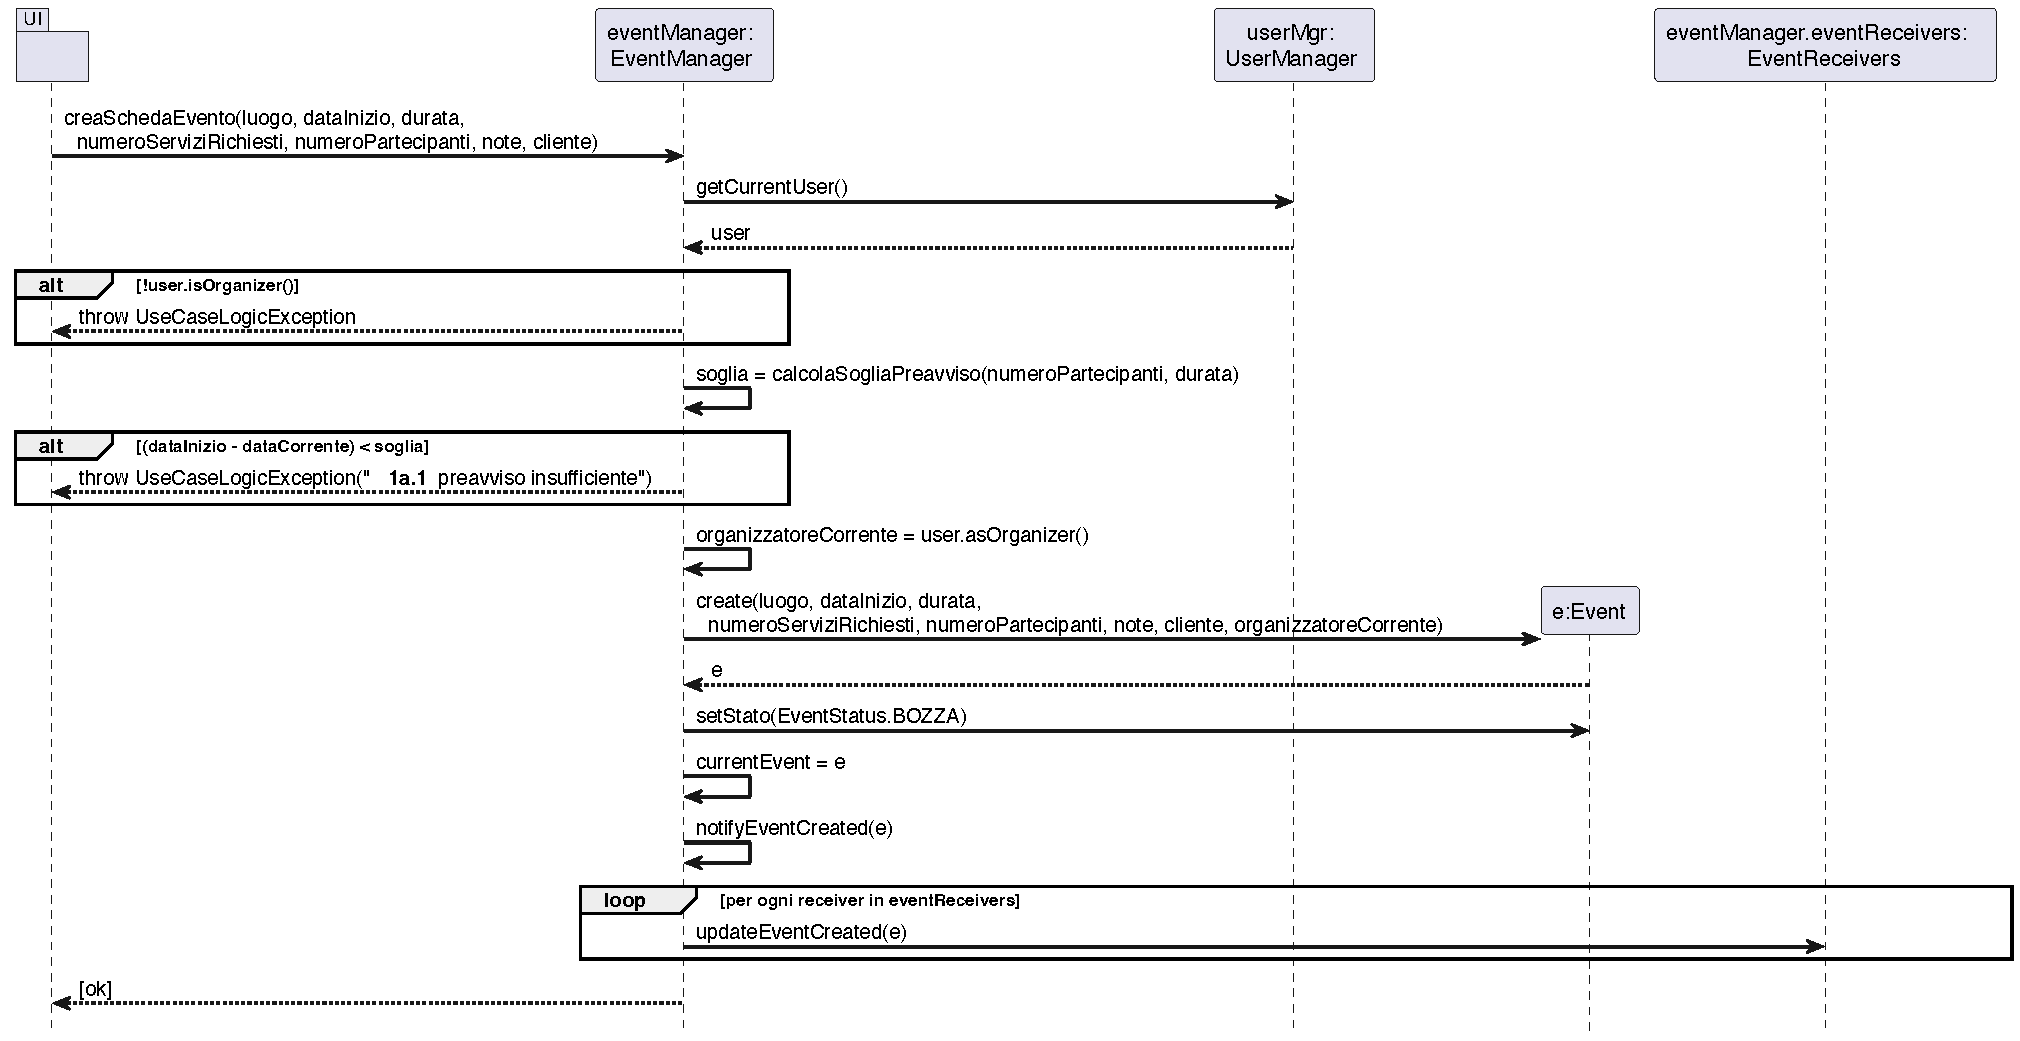
\includegraphics[width=\dsdscreenw, height=\dsdscreenhfirst, keepaspectratio]{dsd/dsd_op1}
\end{figure}

% ─────────────────────────────────────────────────────────────
\clearpage
\dsdpage{595.276}
\section{op2 --- \texttt{apriEvento}}
\label{sec:dsd_op16}

\begin{figure}[H]
  \centering
  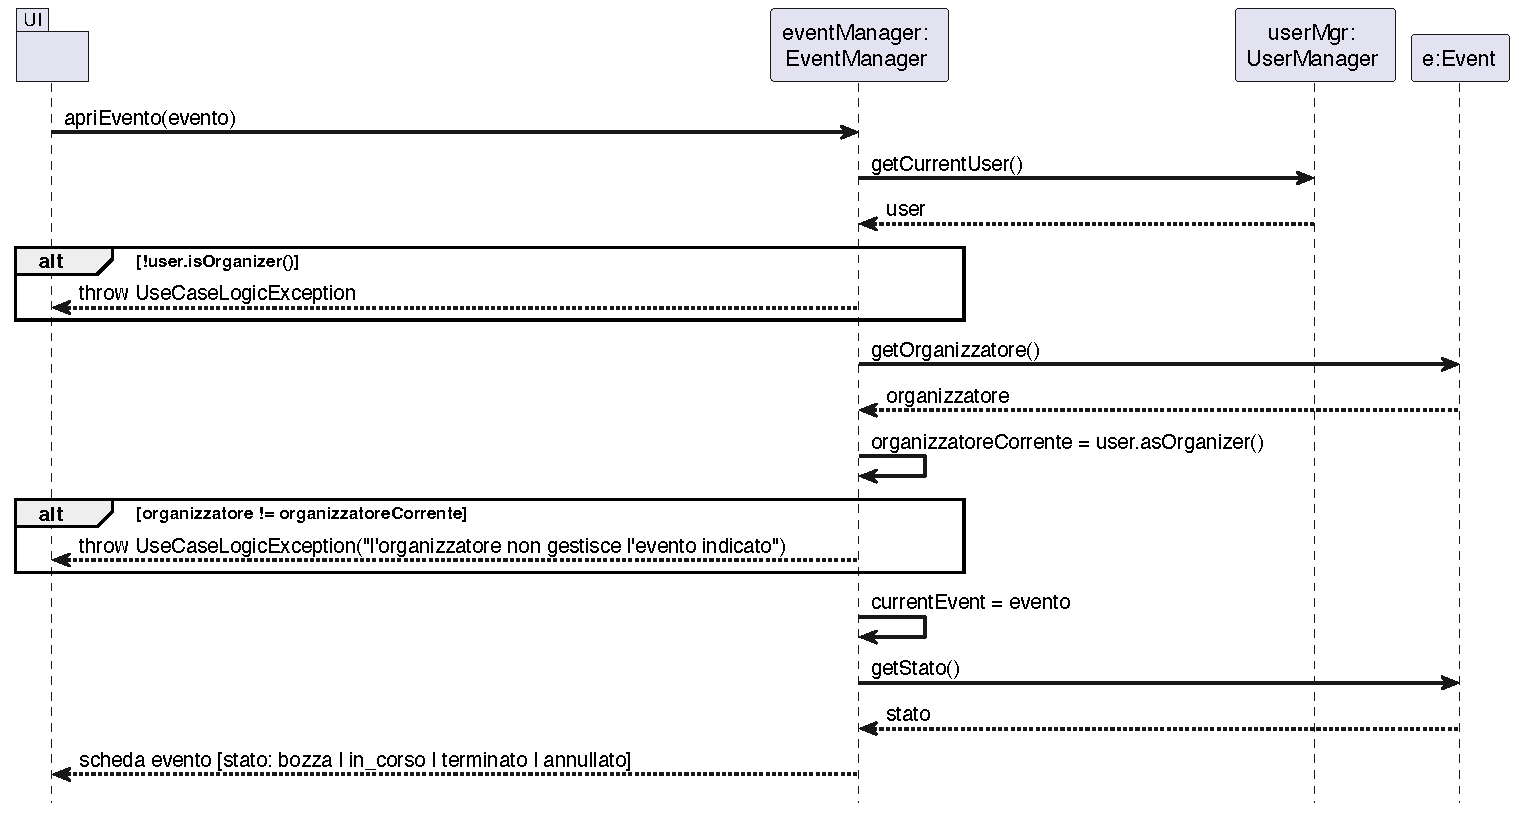
\includegraphics[width=\dsdscreenw, height=\dsdscreenh, keepaspectratio]{dsd/dsd_op16}
\end{figure}

% ─────────────────────────────────────────────────────────────
\clearpage
\dsdpage{595.276}
\section{op3 --- \texttt{creaSchedaEventoRicorrente}}
\label{sec:dsd_op1a}

\begin{figure}[H]
  \centering
  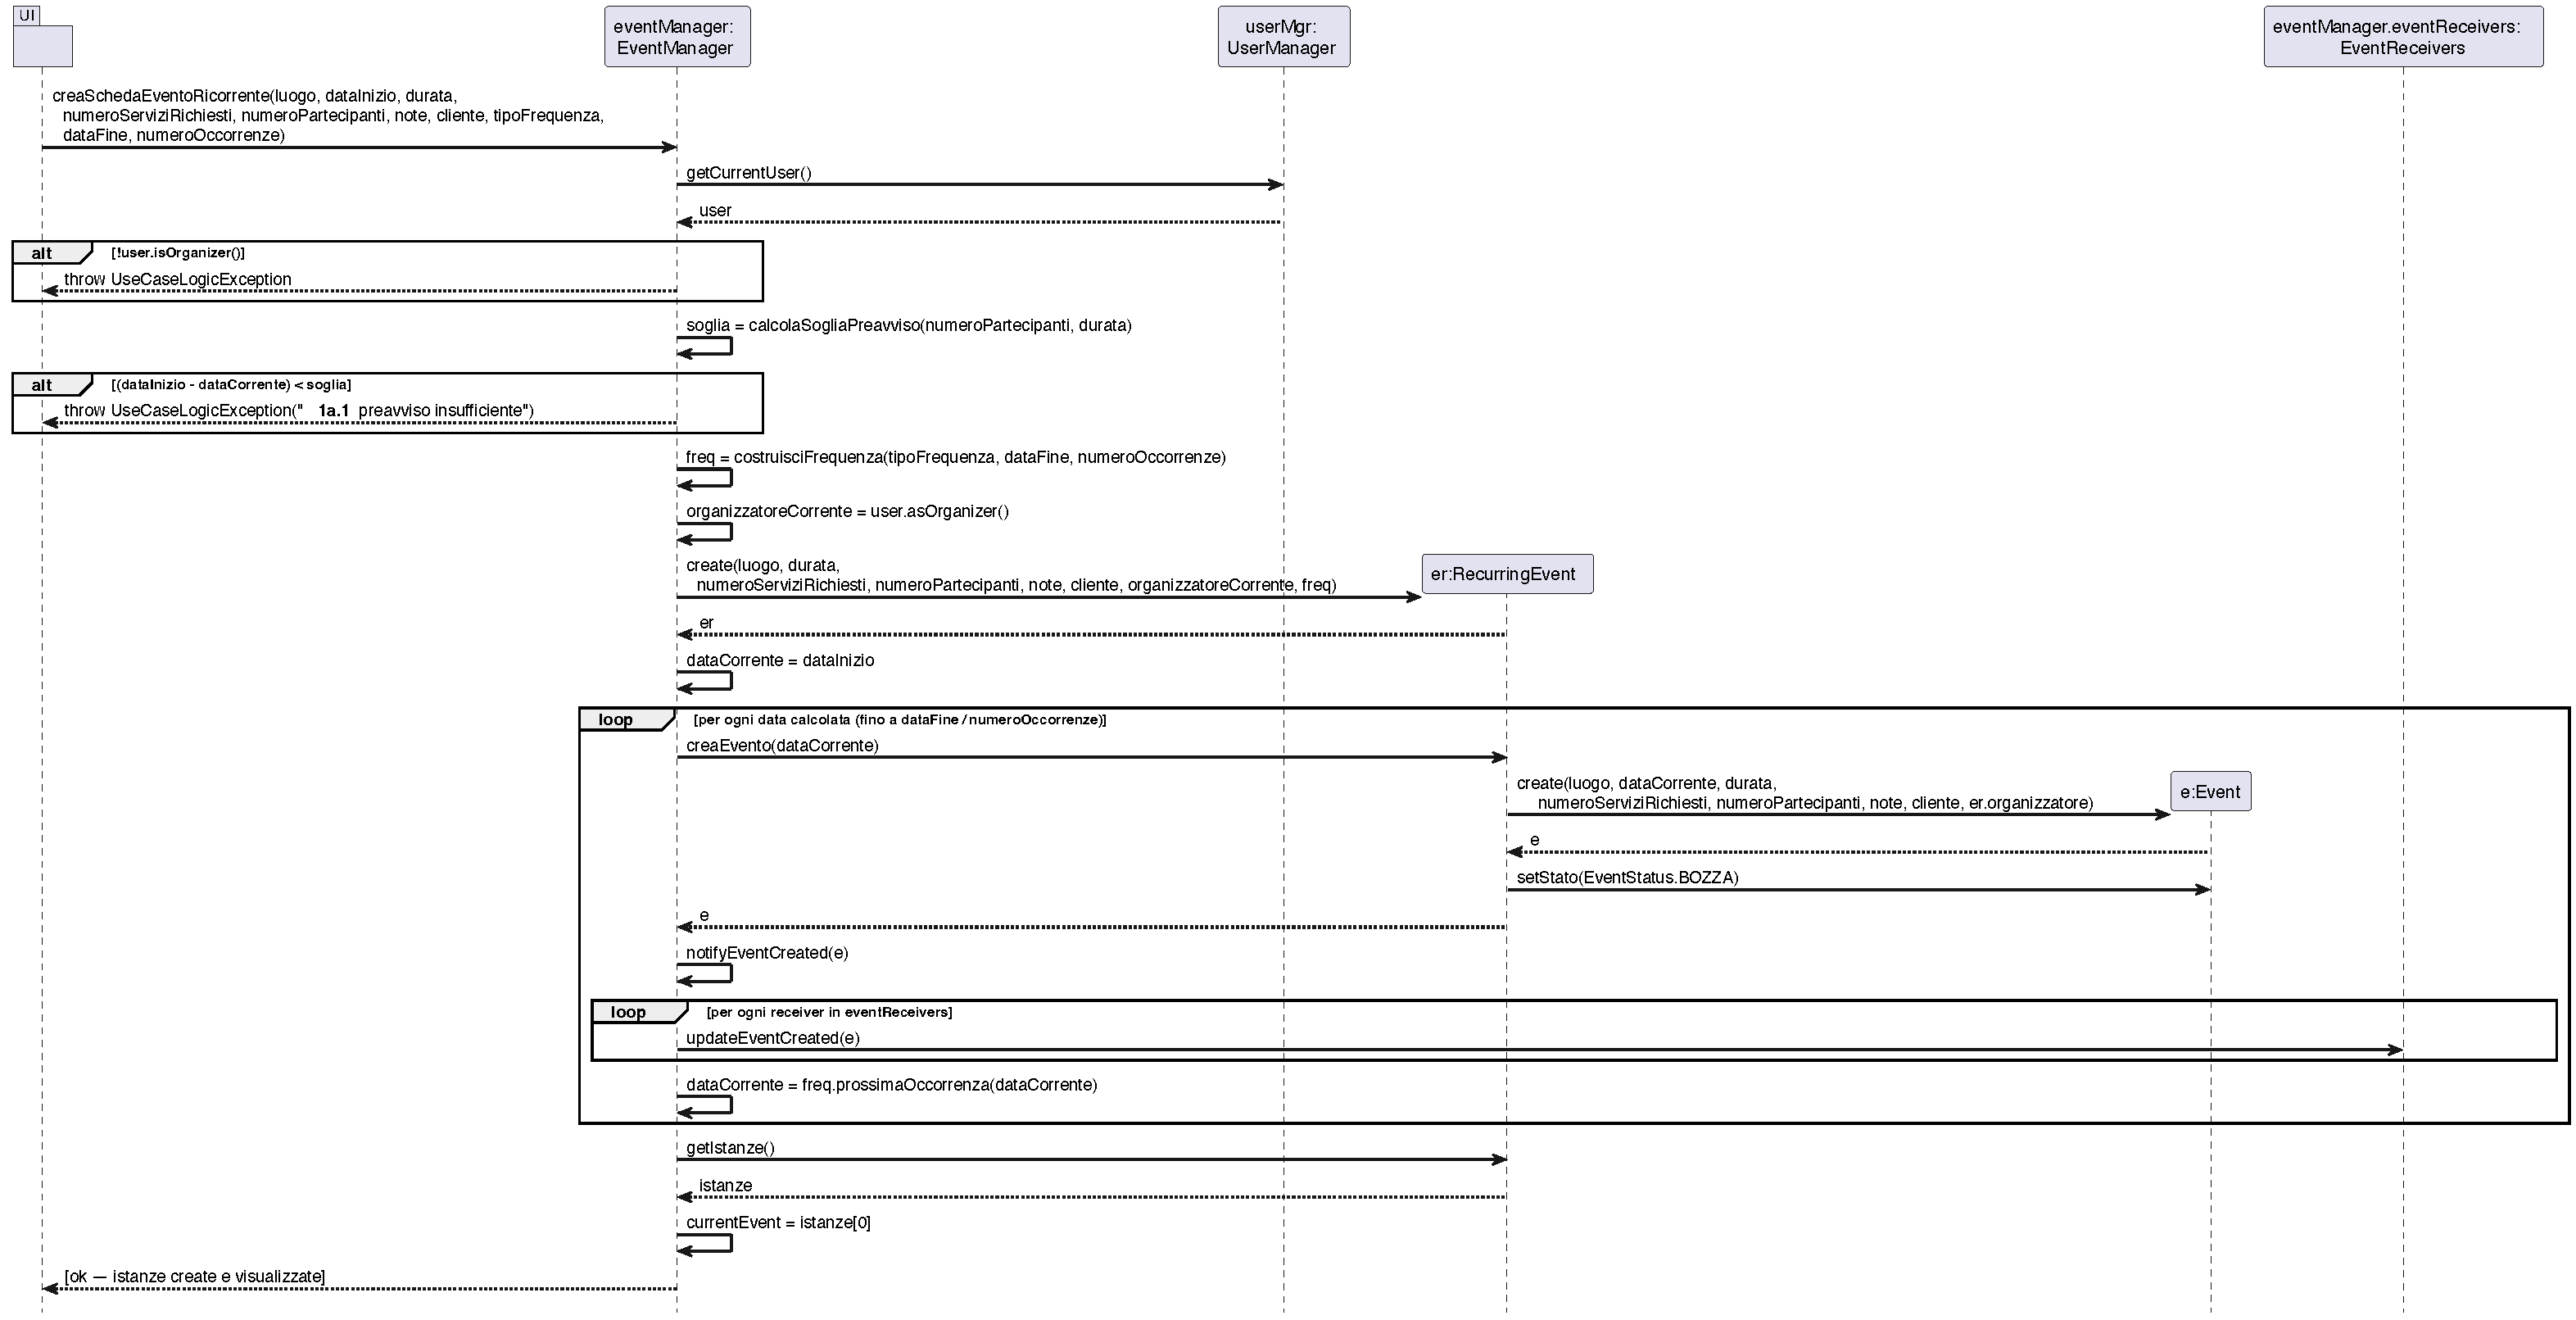
\includegraphics[width=\dsdscreenw, height=\dsdscreenh, keepaspectratio]{dsd/dsd_op1a}
\end{figure}

% ─────────────────────────────────────────────────────────────
\clearpage
\dsdpage{595.276}
\section{op4 --- \texttt{visualizzaStatoCucina}}
\label{sec:dsd_op_cucina}

\begin{figure}[H]
  \centering
  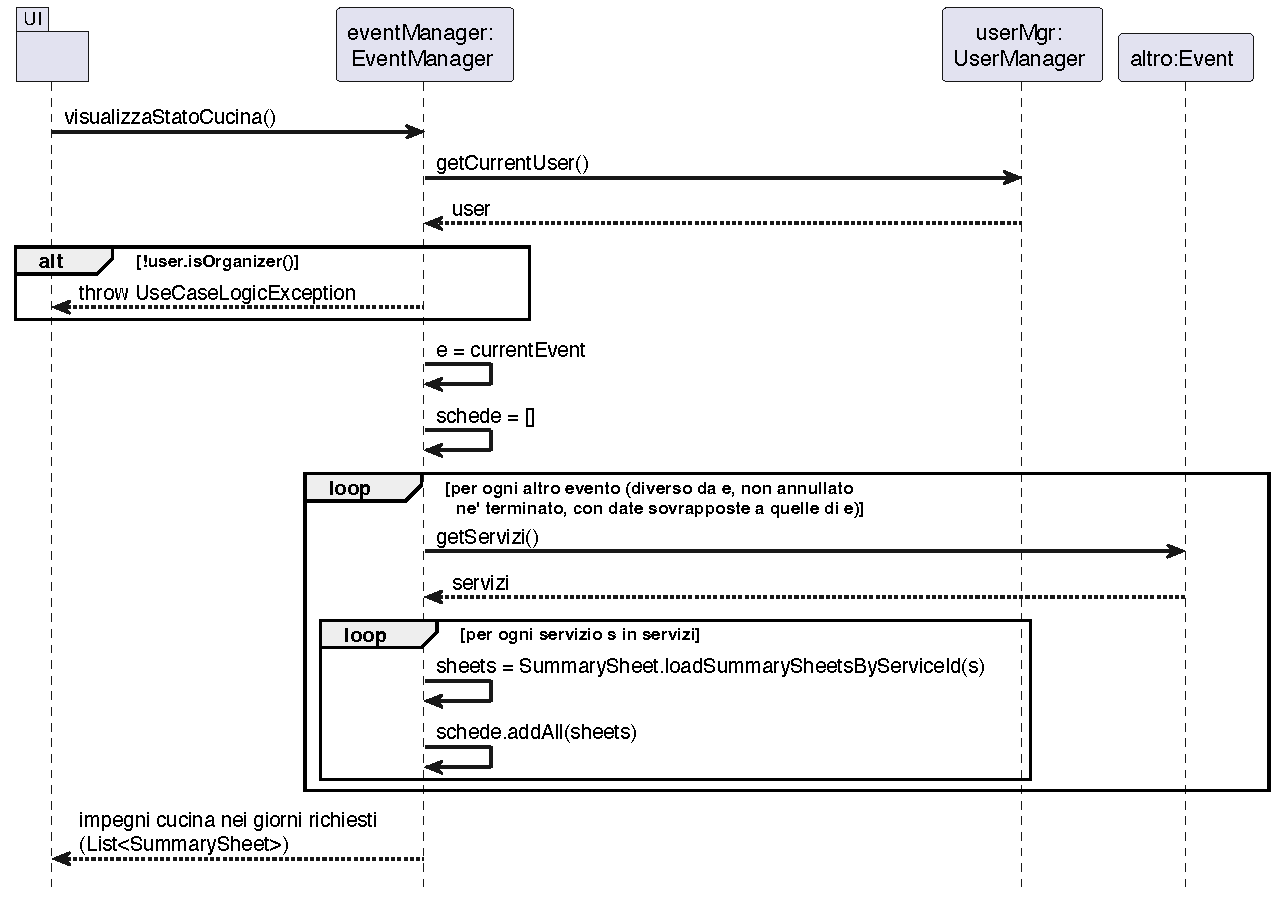
\includegraphics[width=\dsdscreenw, height=\dsdscreenh, keepaspectratio]{dsd/dsd_op_cucina}
\end{figure}

% ─────────────────────────────────────────────────────────────
\clearpage
\dsdpage{780}
\section{op5 --- \texttt{aggiungiServizio} / \texttt{inserisciTurnoServizio}}
\label{sec:dsd_op17}

\begin{figure}[H]
  \centering
  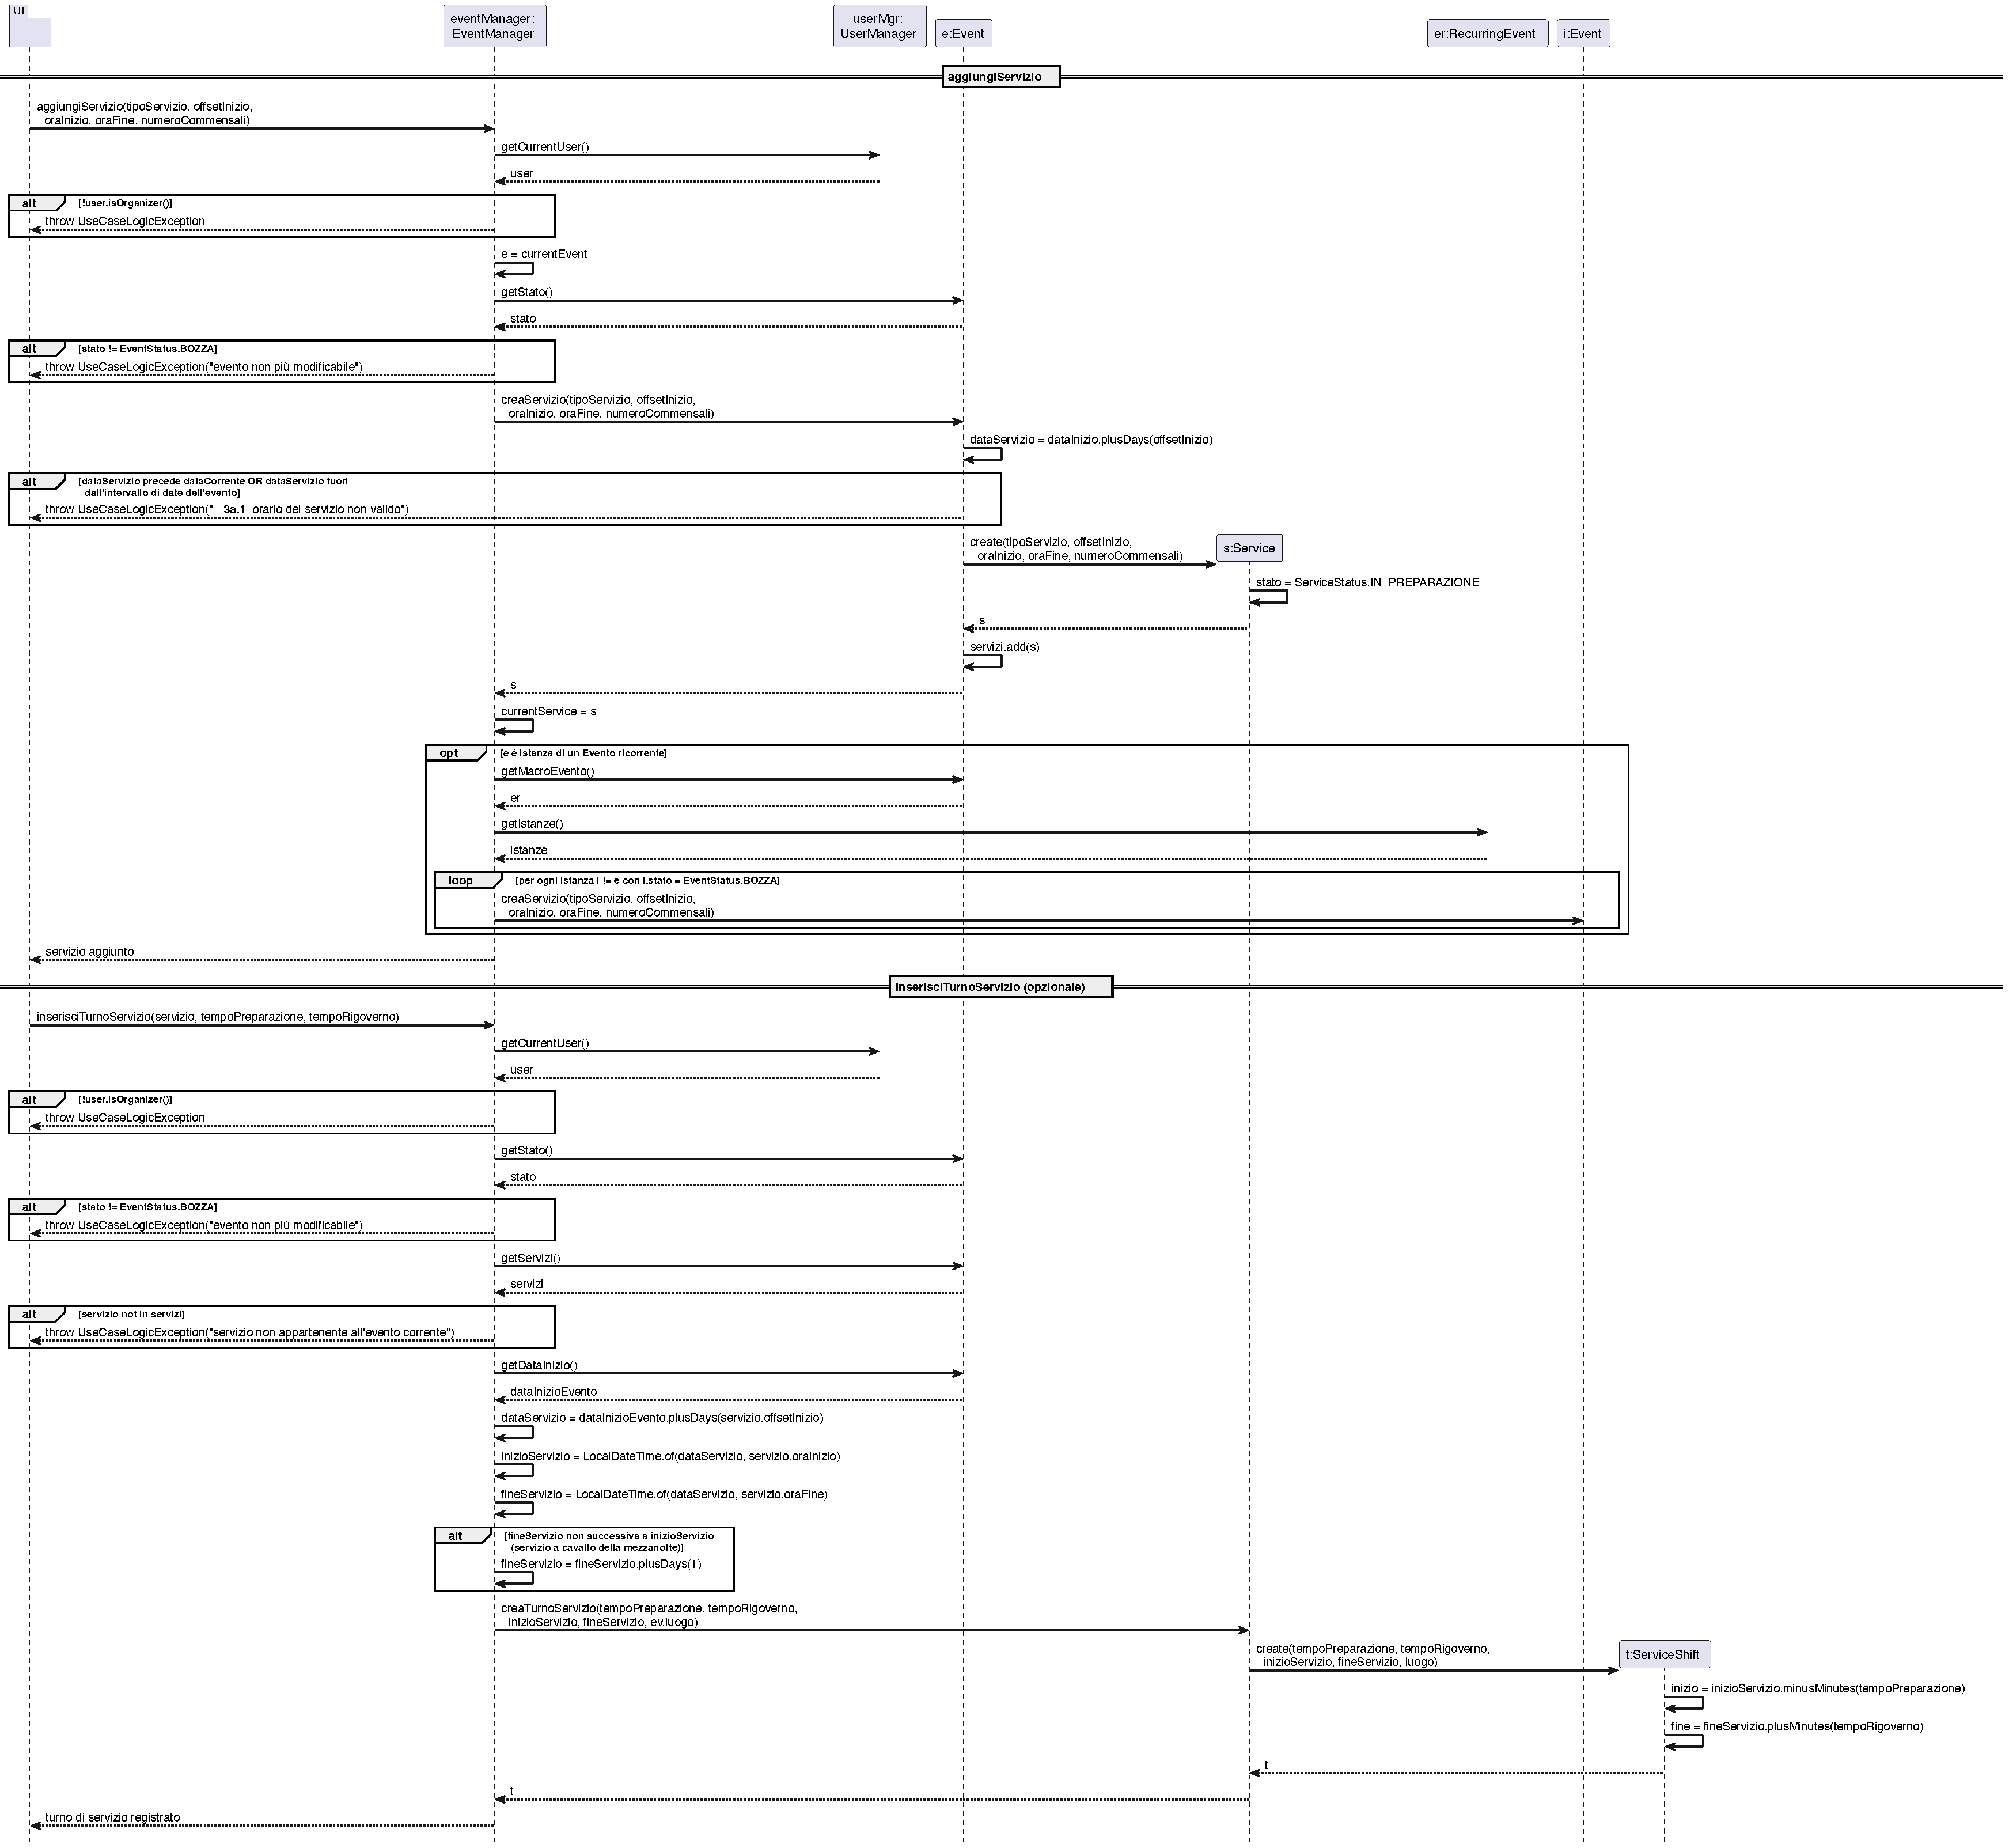
\includegraphics[width=\dsdscreenw, height=655pt, keepaspectratio]{dsd/dsd_op17}
\end{figure}

% ─────────────────────────────────────────────────────────────
\clearpage
\dsdpage{595.276}
\section{op6 --- \texttt{assegnaChef}}
\label{sec:dsd_op2}

\begin{figure}[H]
  \centering
  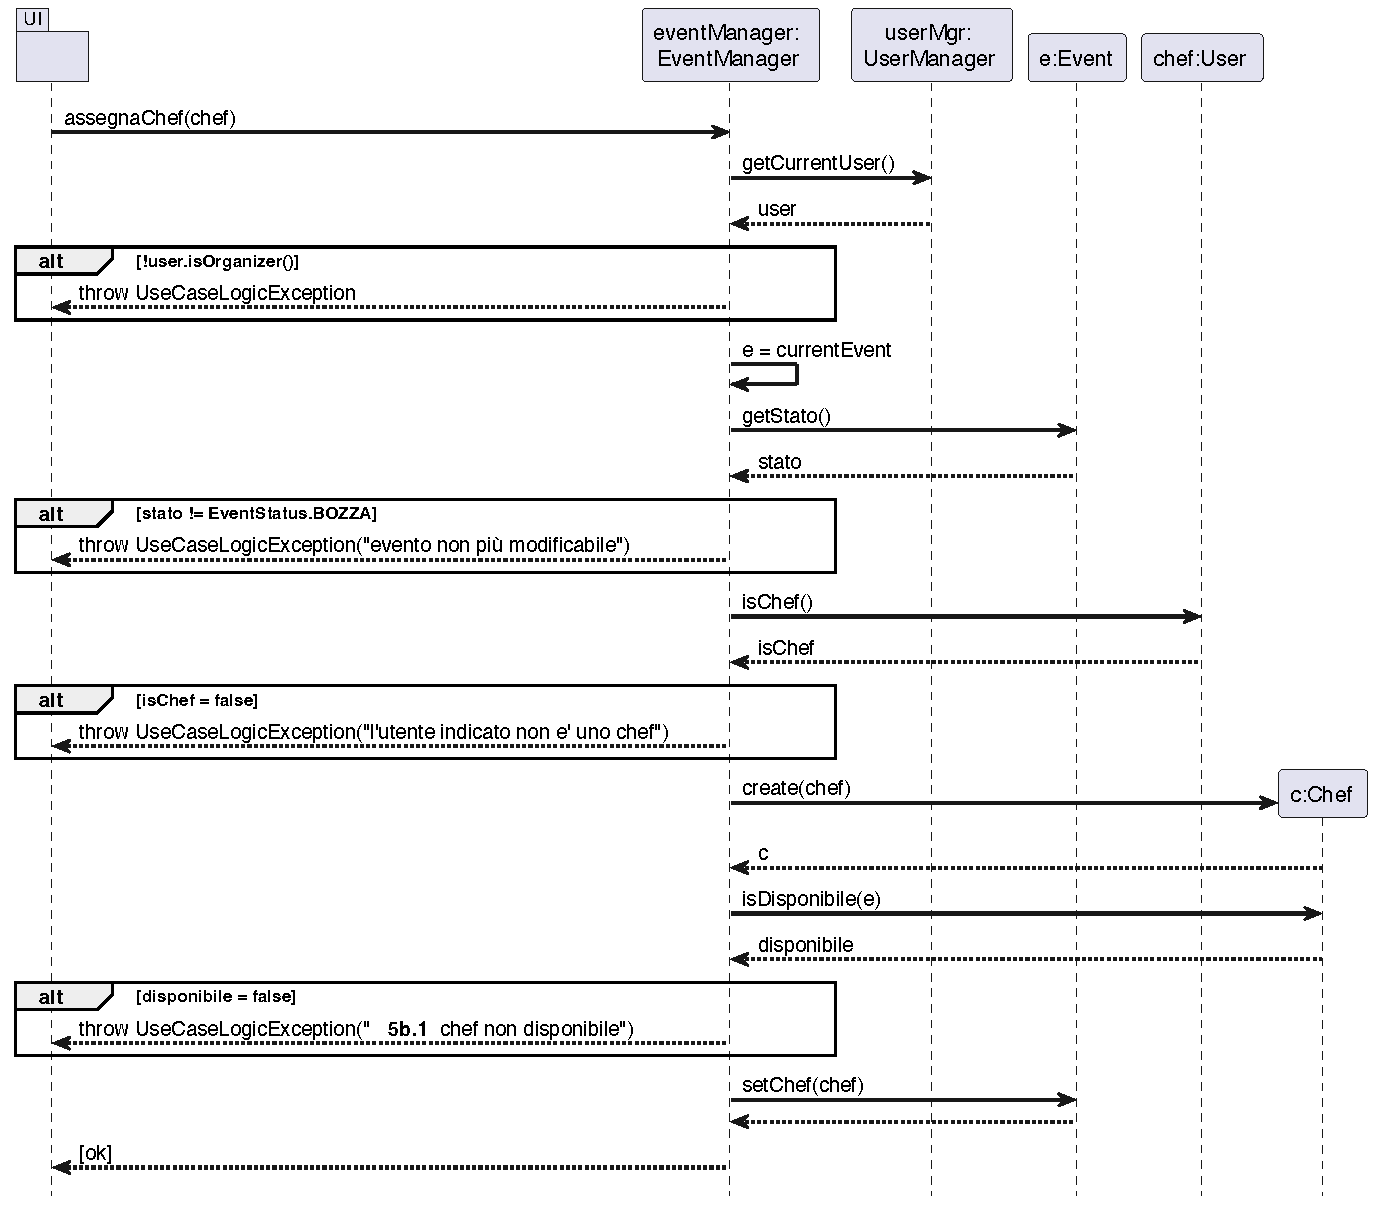
\includegraphics[width=\dsdscreenw, height=\dsdscreenh, keepaspectratio]{dsd/dsd_op2}
\end{figure}

% ─────────────────────────────────────────────────────────────
\clearpage
\dsdpage{920}
\section{op7 --- \texttt{approvaMenu}}
\label{sec:dsd_op3}

\begin{center}
  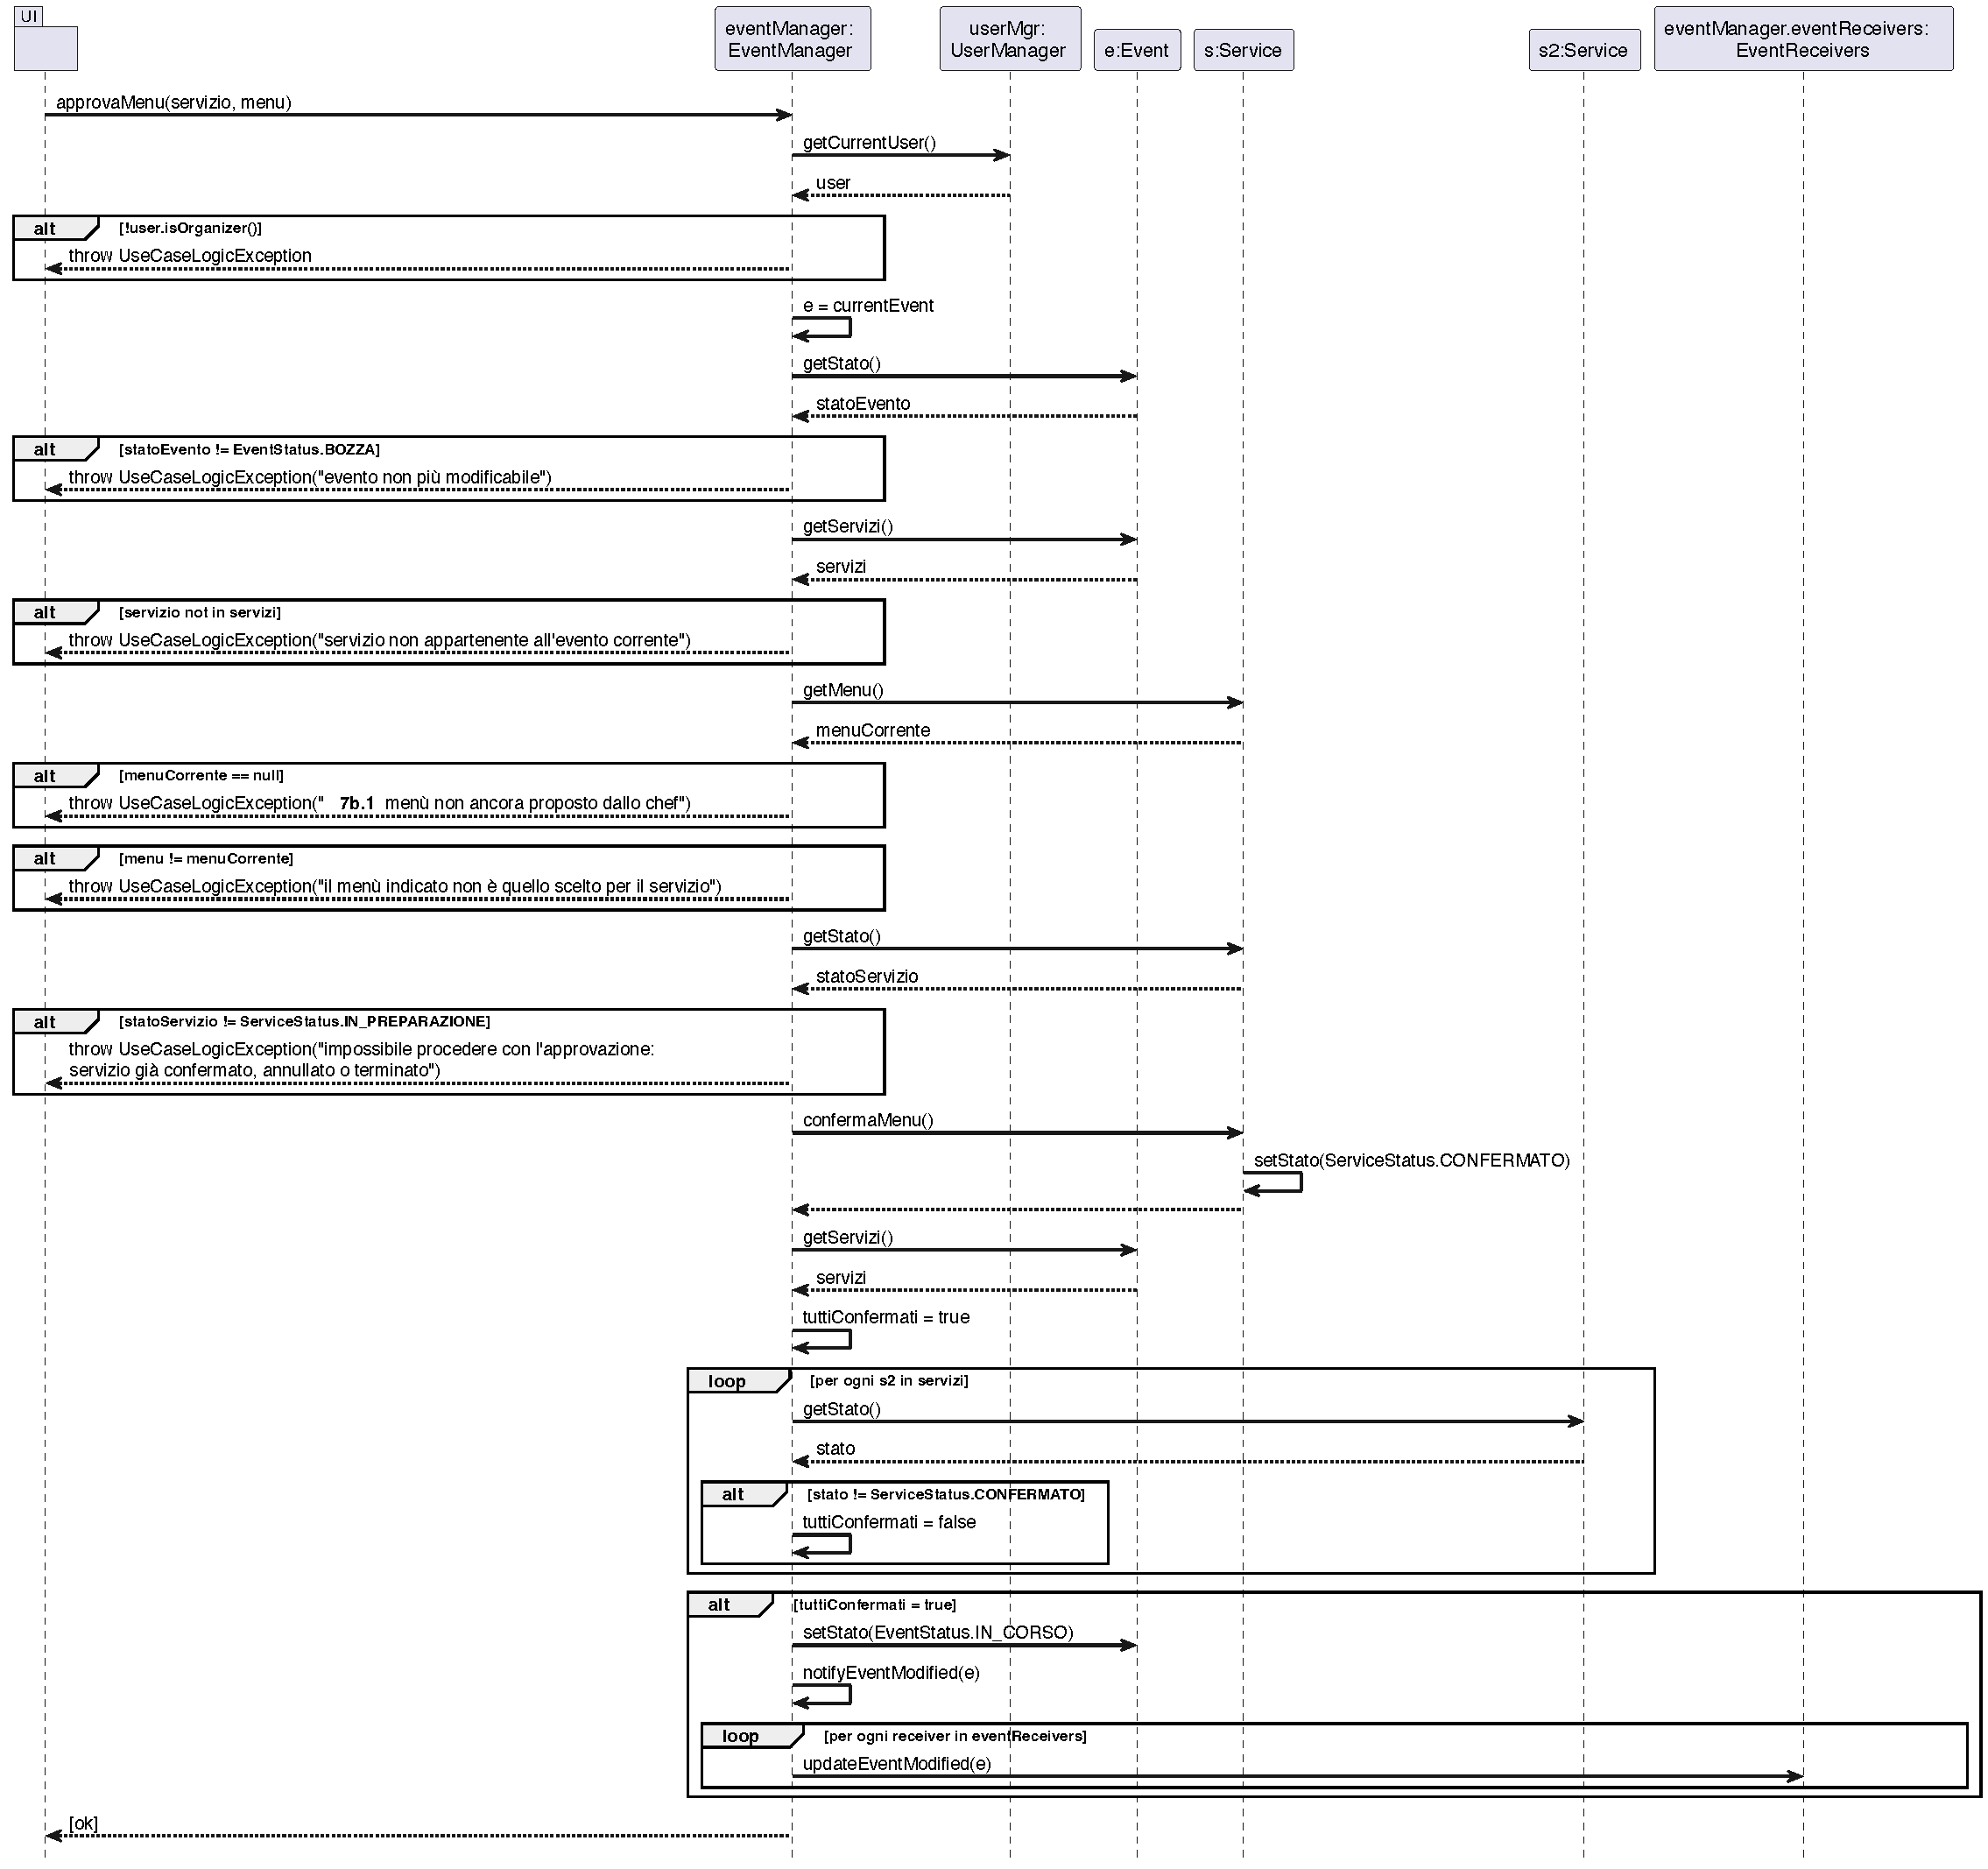
\includegraphics[width=\dsdscreenw, height=795pt, keepaspectratio]{dsd/dsd_op3}
\end{center}

% ─────────────────────────────────────────────────────────────
\clearpage
\dsdpage{595.276}
\section{op8 --- \texttt{assegnaPersonaleATurno}}
\label{sec:dsd_op4}

\begin{figure}[H]
  \centering
  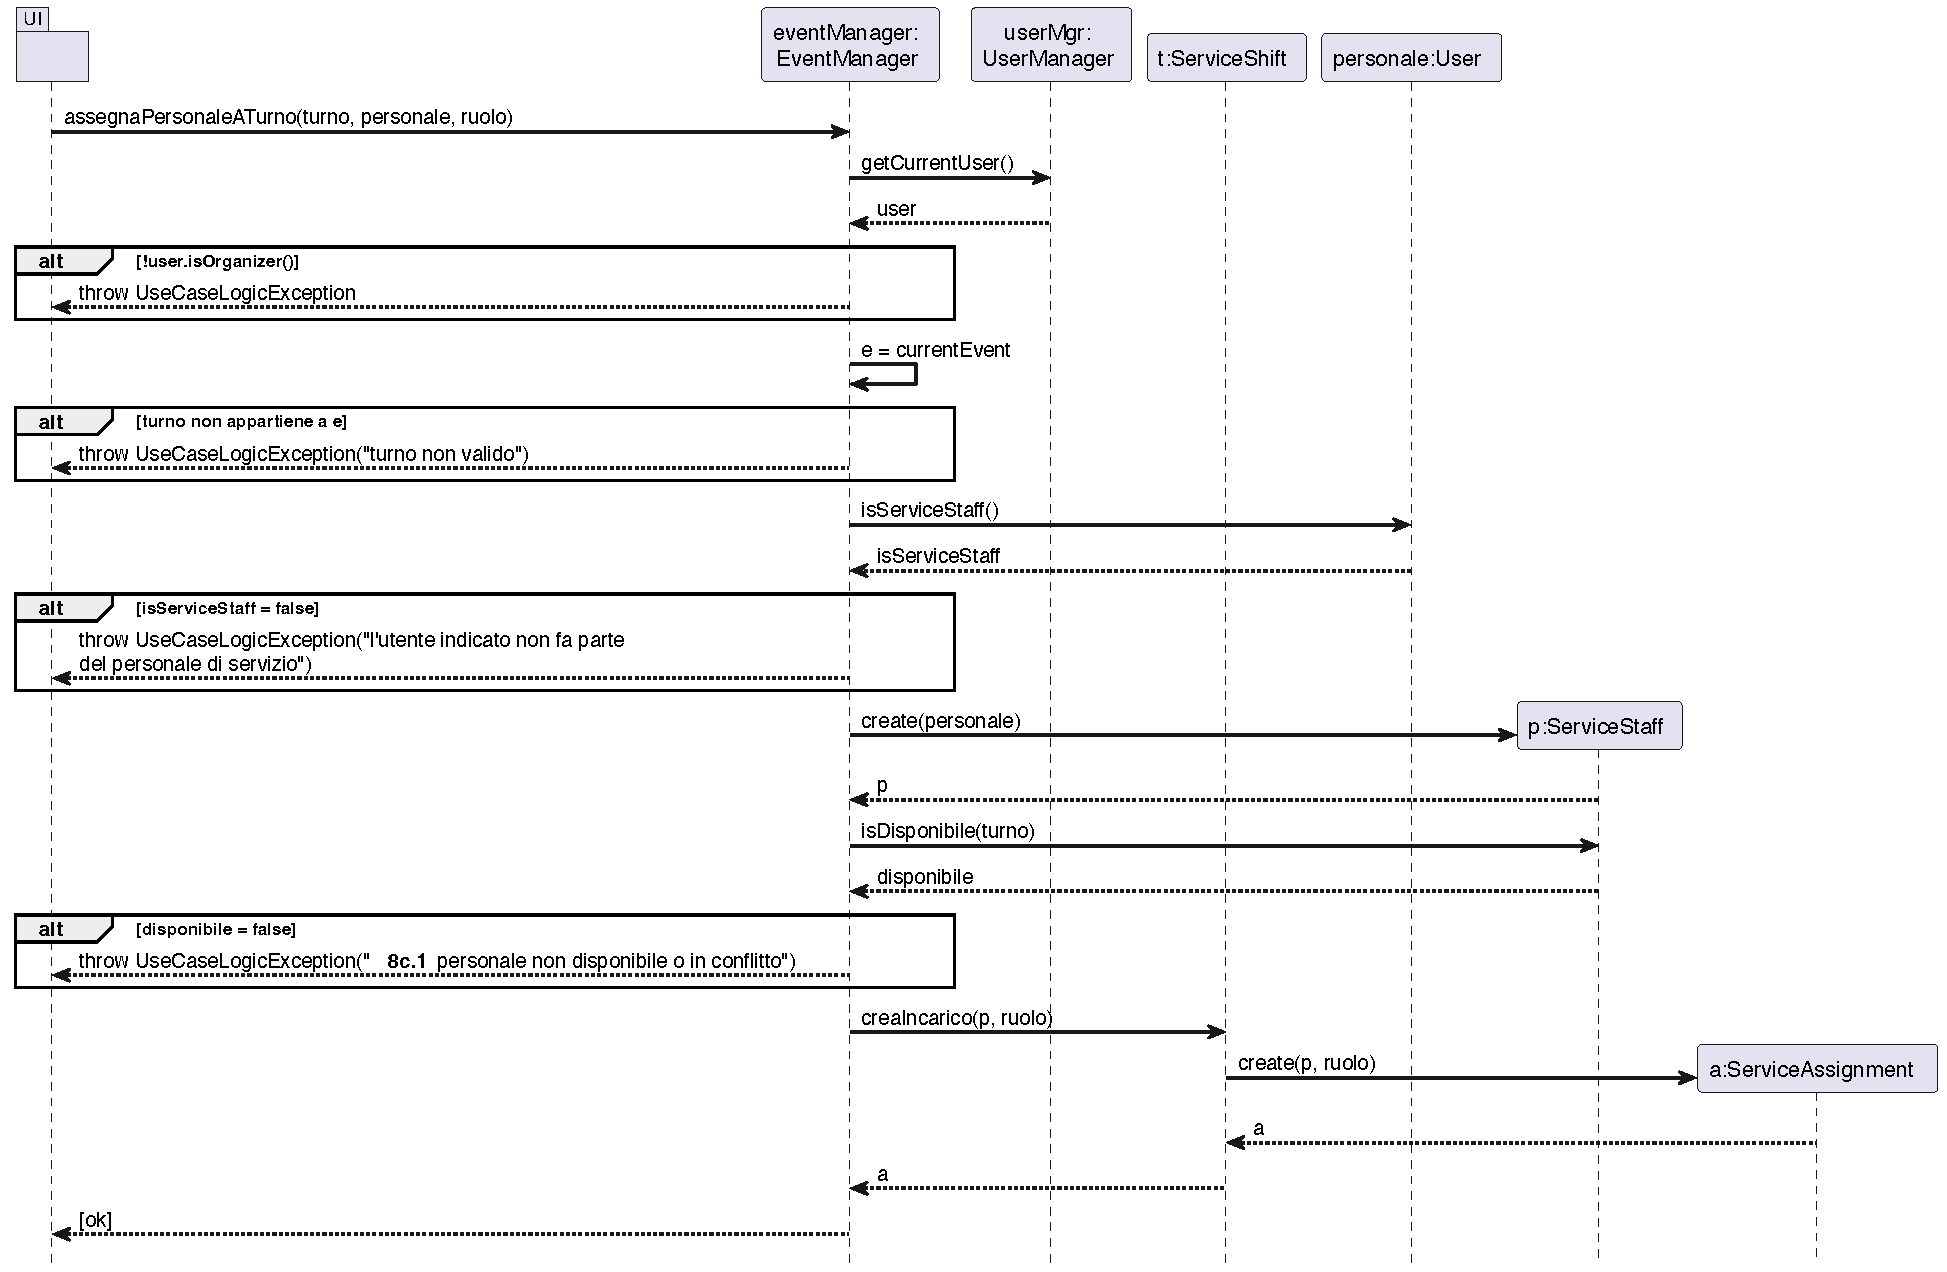
\includegraphics[width=\dsdscreenw, height=\dsdscreenh, keepaspectratio]{dsd/dsd_op4}
\end{figure}

% ─────────────────────────────────────────────────────────────
\clearpage
\dsdpage{595.276}
\section{op9 --- \texttt{chiudiEvento}}
\label{sec:dsd_op5}

\begin{figure}[H]
  \centering
  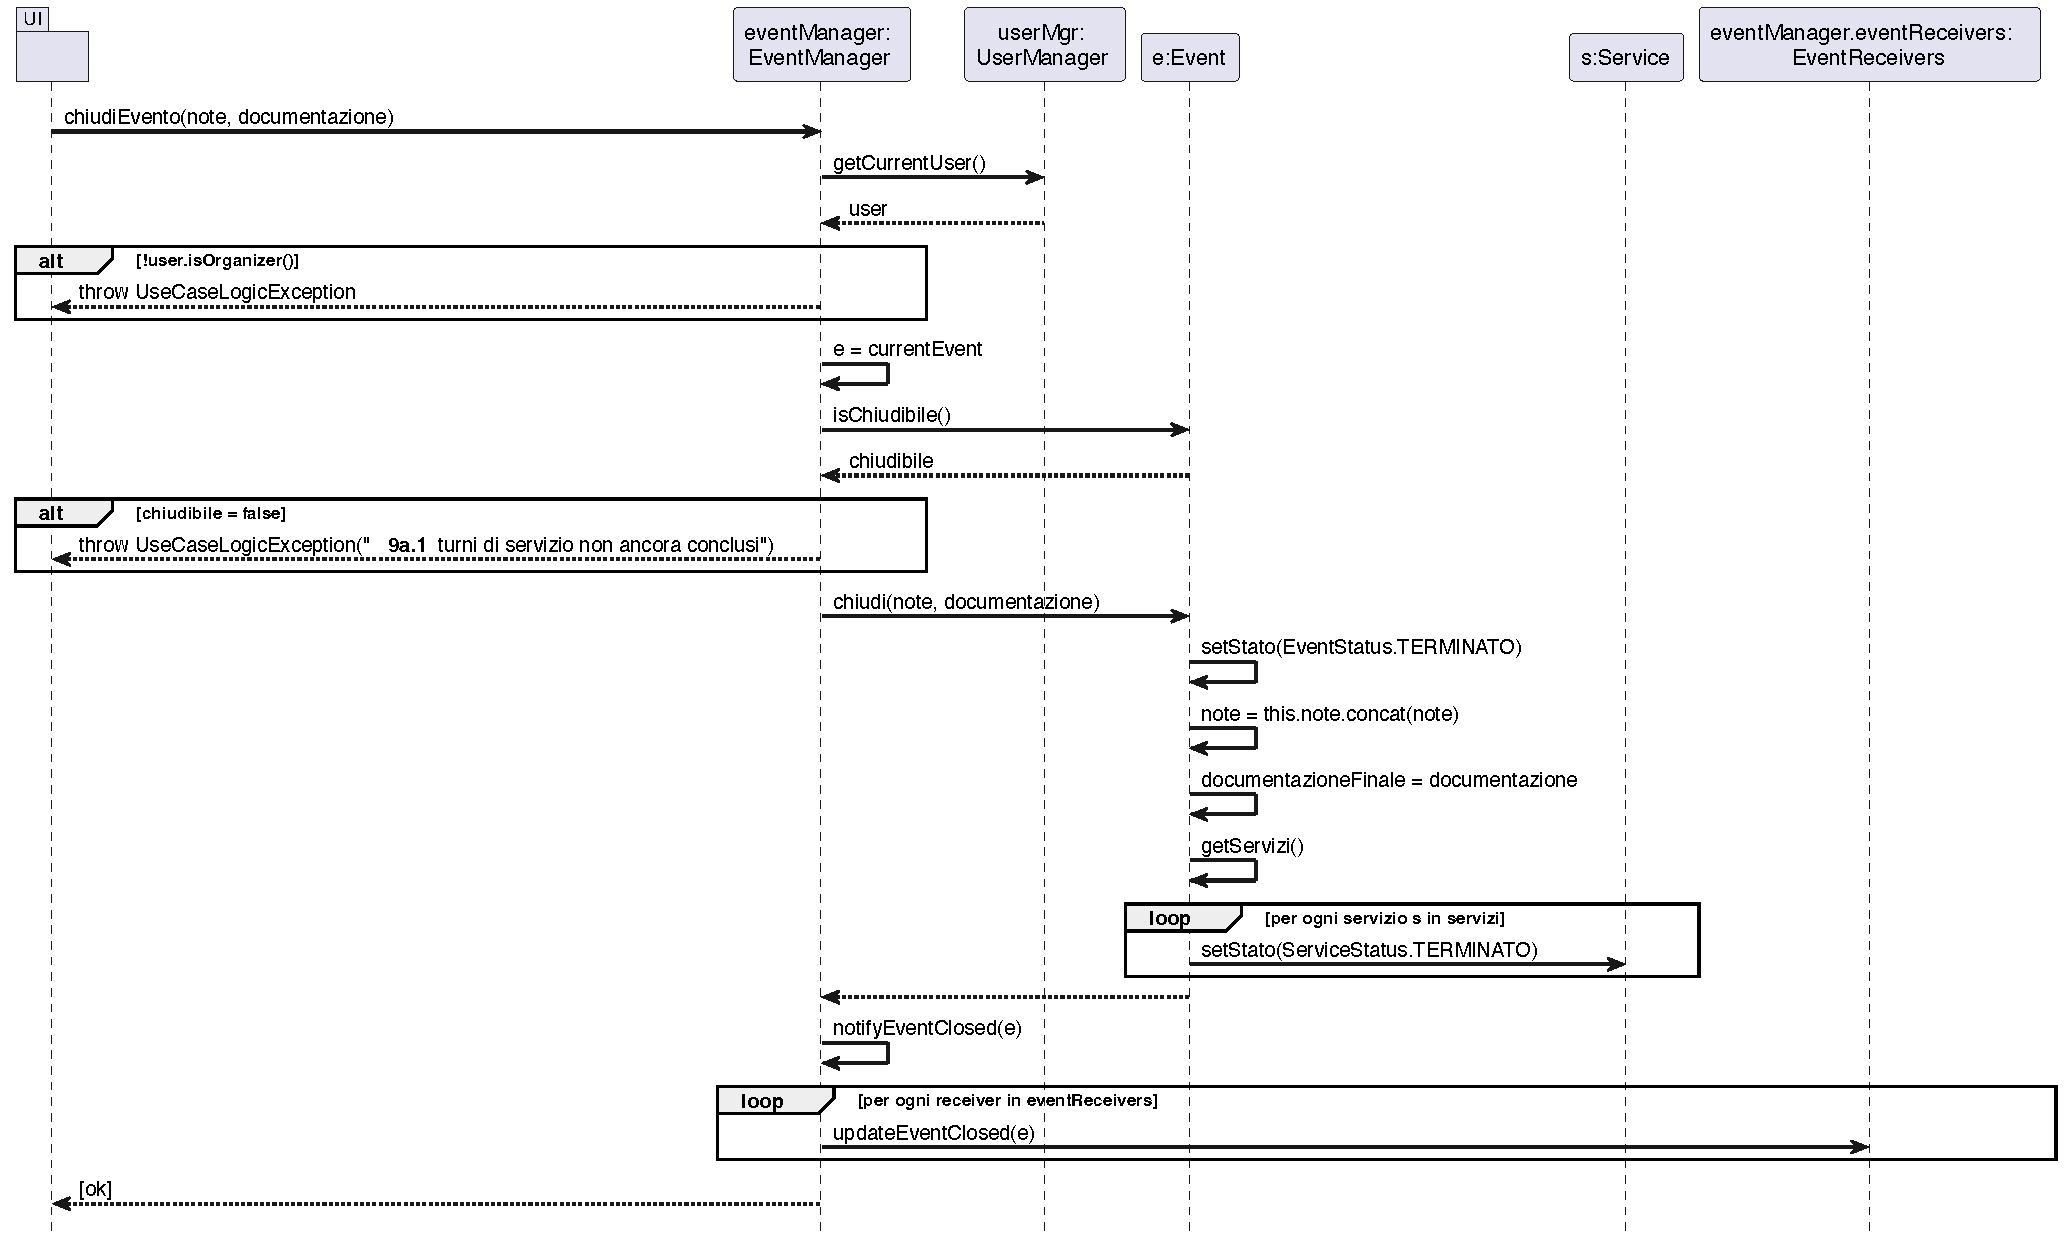
\includegraphics[width=\dsdscreenw, height=\dsdscreenh, keepaspectratio]{dsd/dsd_op5}
\end{figure}

% ─────────────────────────────────────────────────────────────
\clearpage
\dsdpage{1080}
\section{op10 --- \texttt{eliminaEvento} / \texttt{annullaEvento}}
\label{sec:dsd_op6}

\begin{figure}[H]
  \centering
  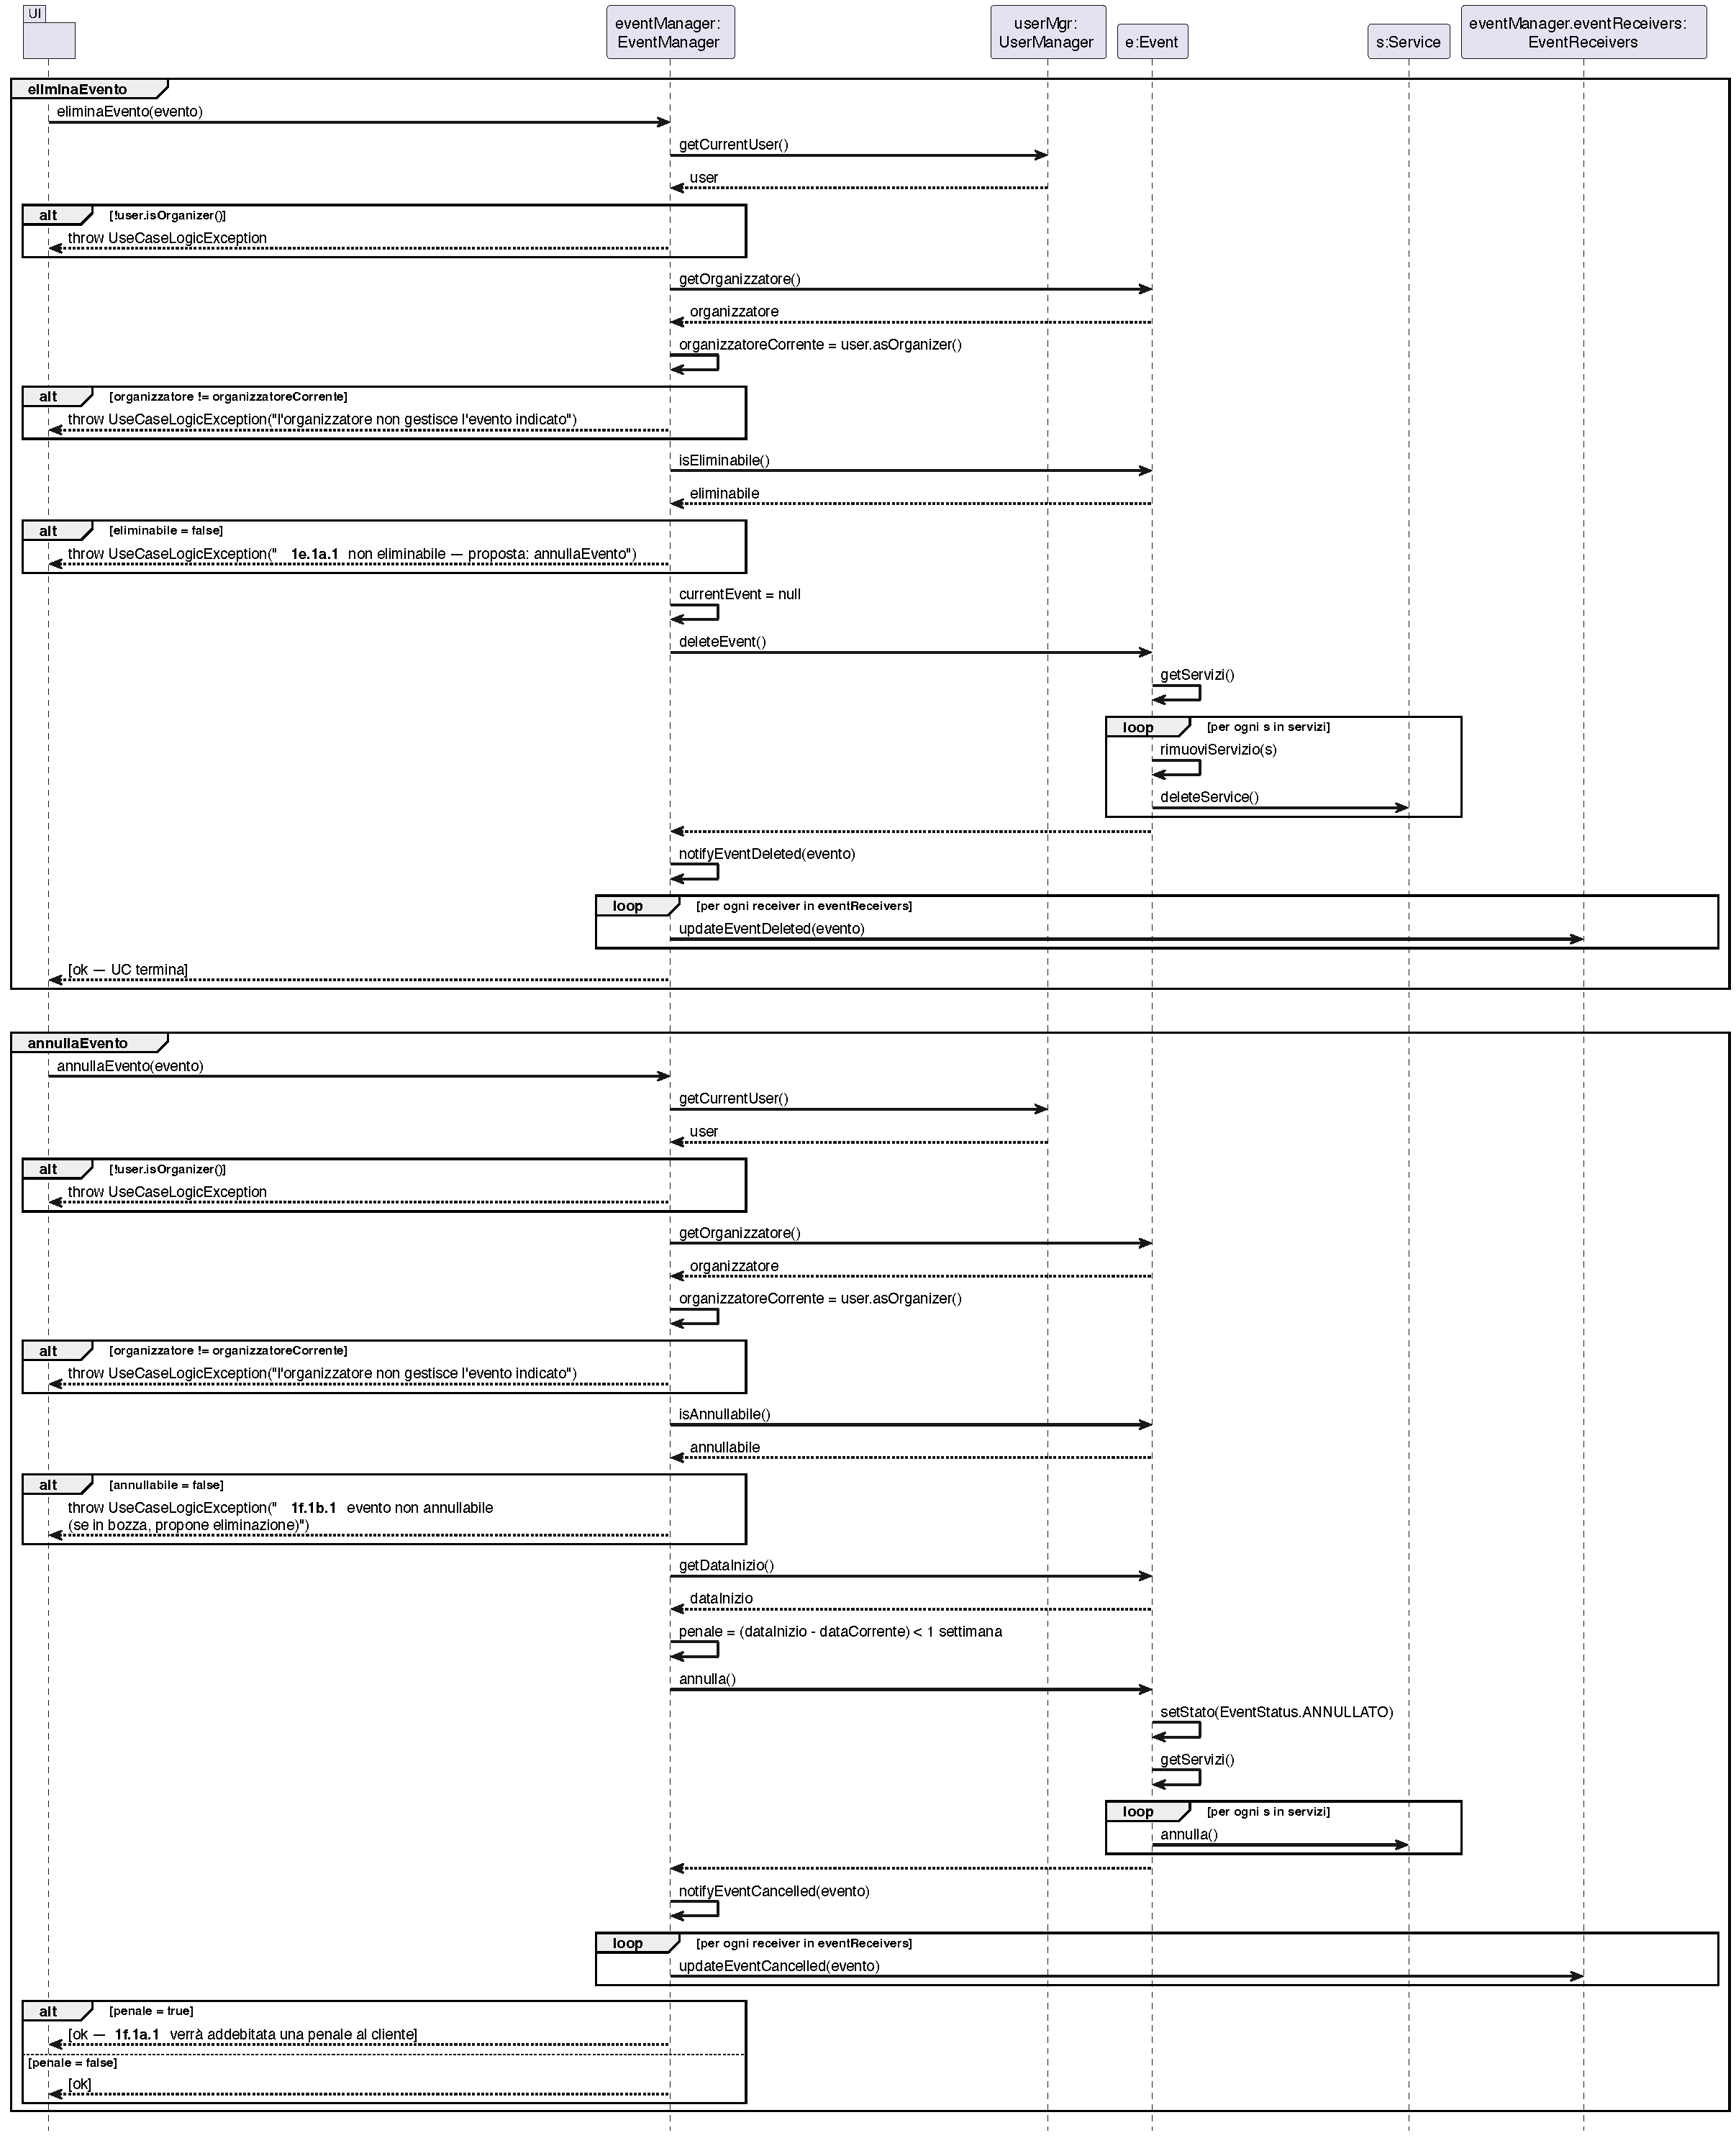
\includegraphics[width=\dsdscreenw, height=955pt, keepaspectratio]{dsd/dsd_op6}
\end{figure}

% ─────────────────────────────────────────────────────────────
\clearpage
\dsdpage{595.276}
\section{op11 --- \texttt{modificaSchedaEvento}}
\label{sec:dsd_op7}

\begin{figure}[H]
  \centering
  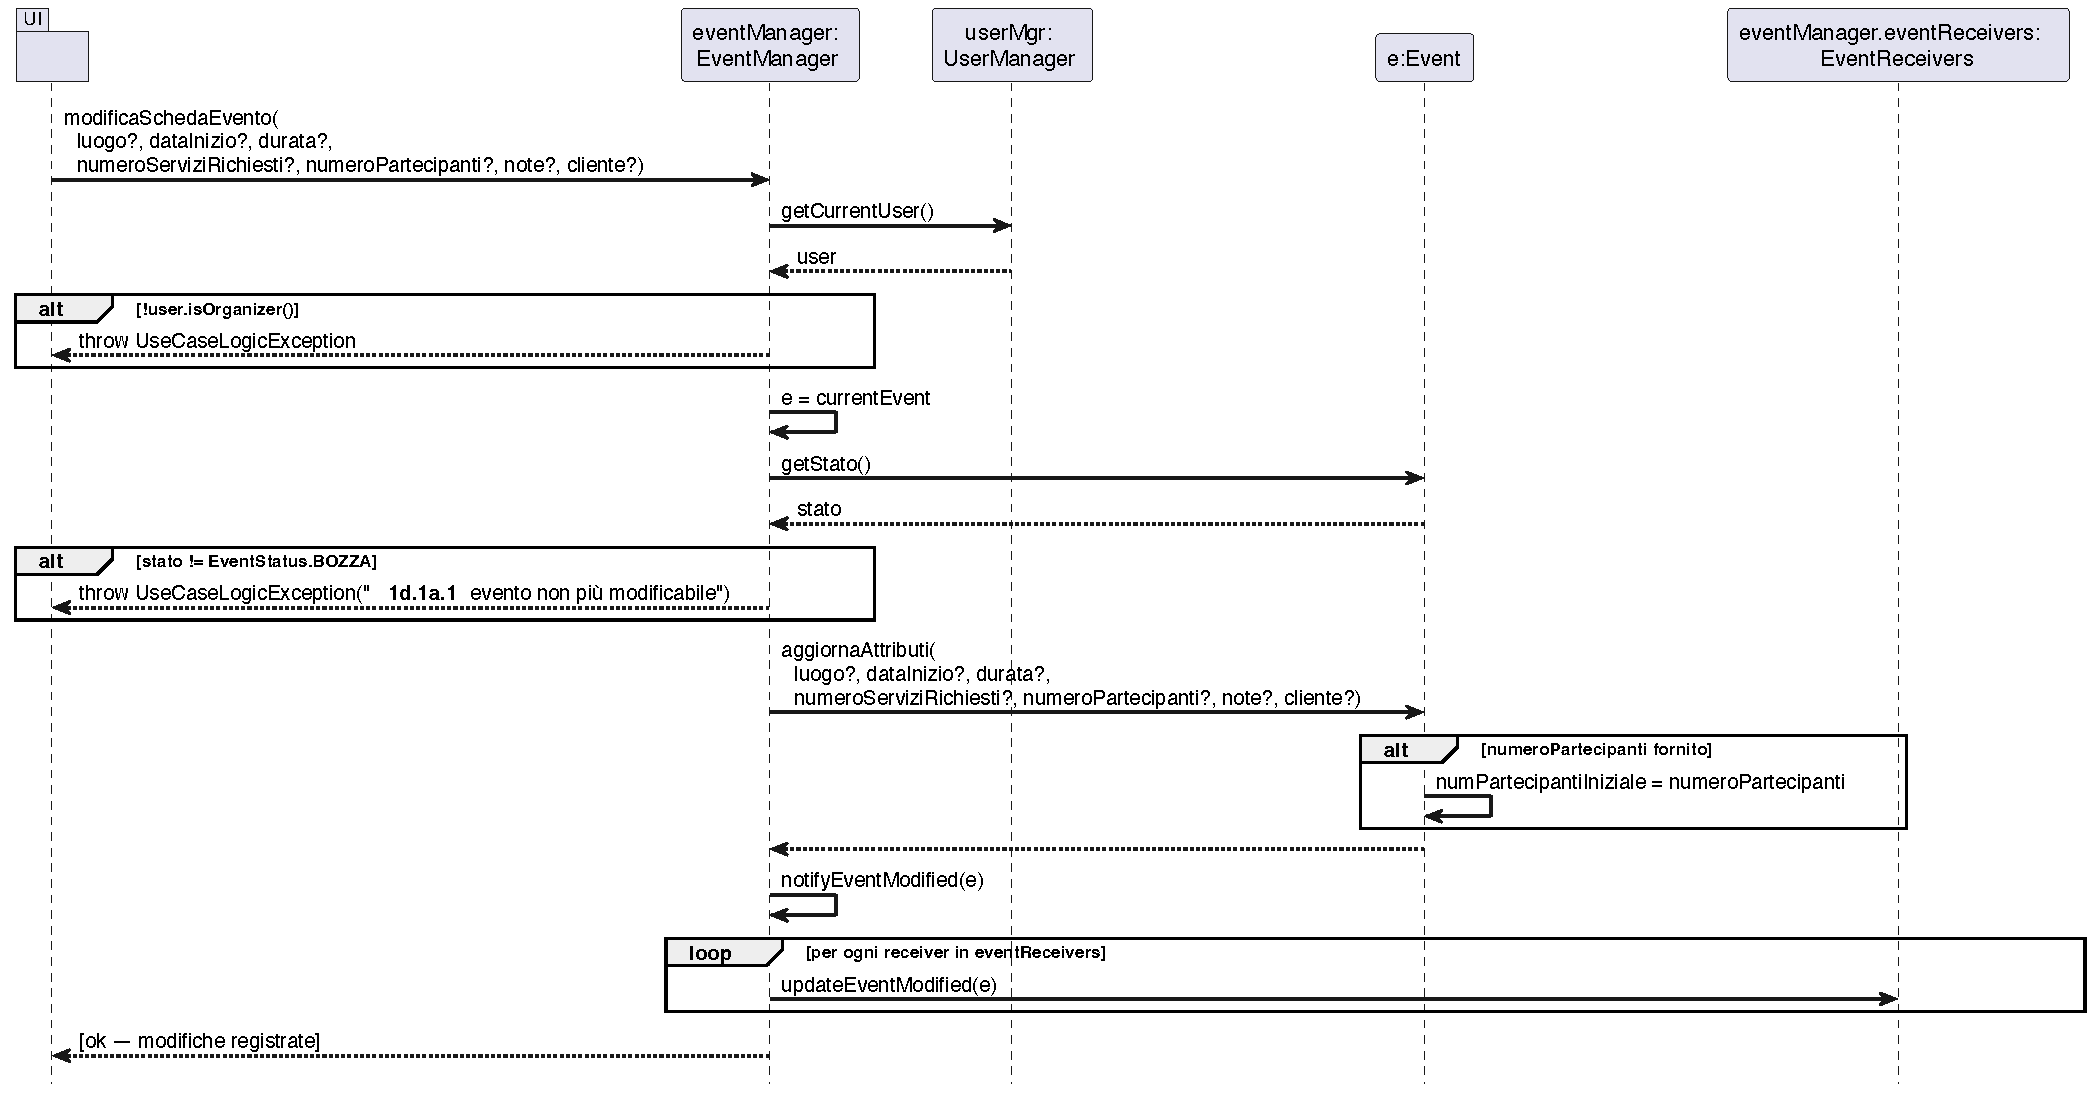
\includegraphics[width=\dsdscreenw, height=\dsdscreenh, keepaspectratio]{dsd/dsd_op7}
\end{figure}

% ─────────────────────────────────────────────────────────────
\clearpage
\dsdpage{595.276}
\section{op12 --- \texttt{rimuoviServizio}}
\label{sec:dsd_op18}

\begin{figure}[H]
  \centering
  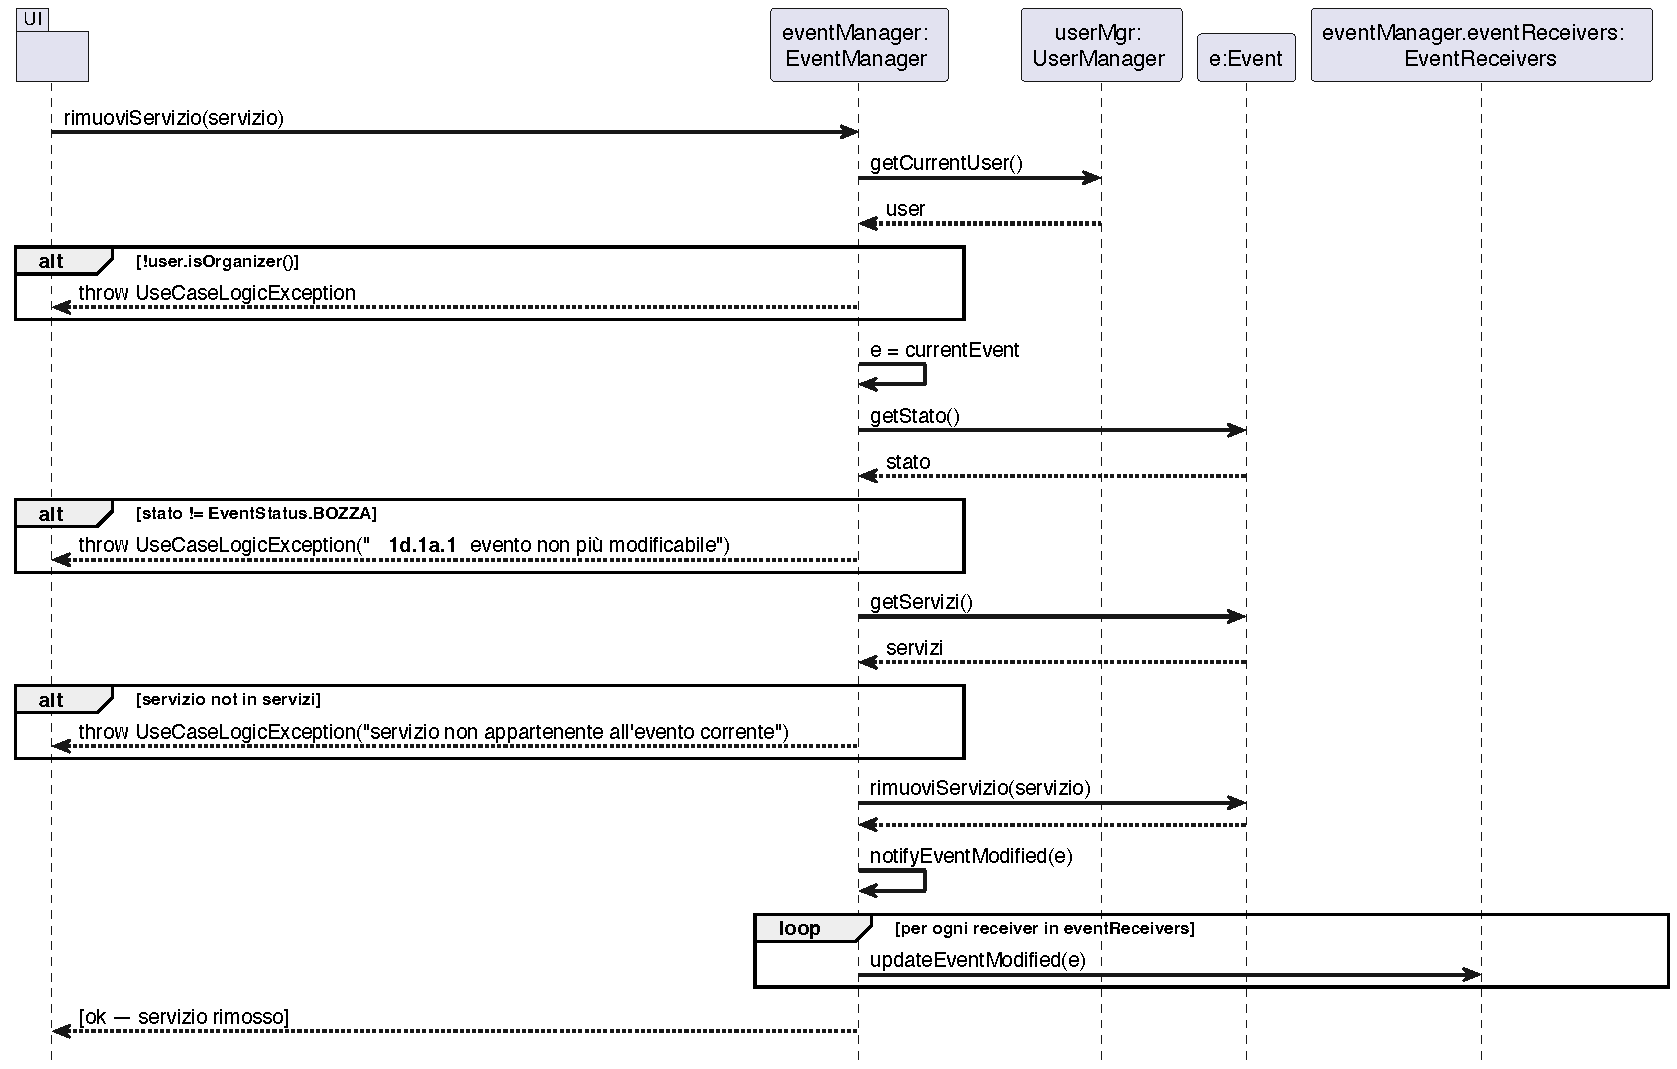
\includegraphics[width=\dsdscreenw, height=\dsdscreenh, keepaspectratio]{dsd/dsd_op18}
\end{figure}

% ─────────────────────────────────────────────────────────────
\clearpage
\dsdpage{595.276}
\section{op13 --- \texttt{modificaSchedaEventoInCorso}}
\label{sec:dsd_op15}

\begin{figure}[H]
  \centering
  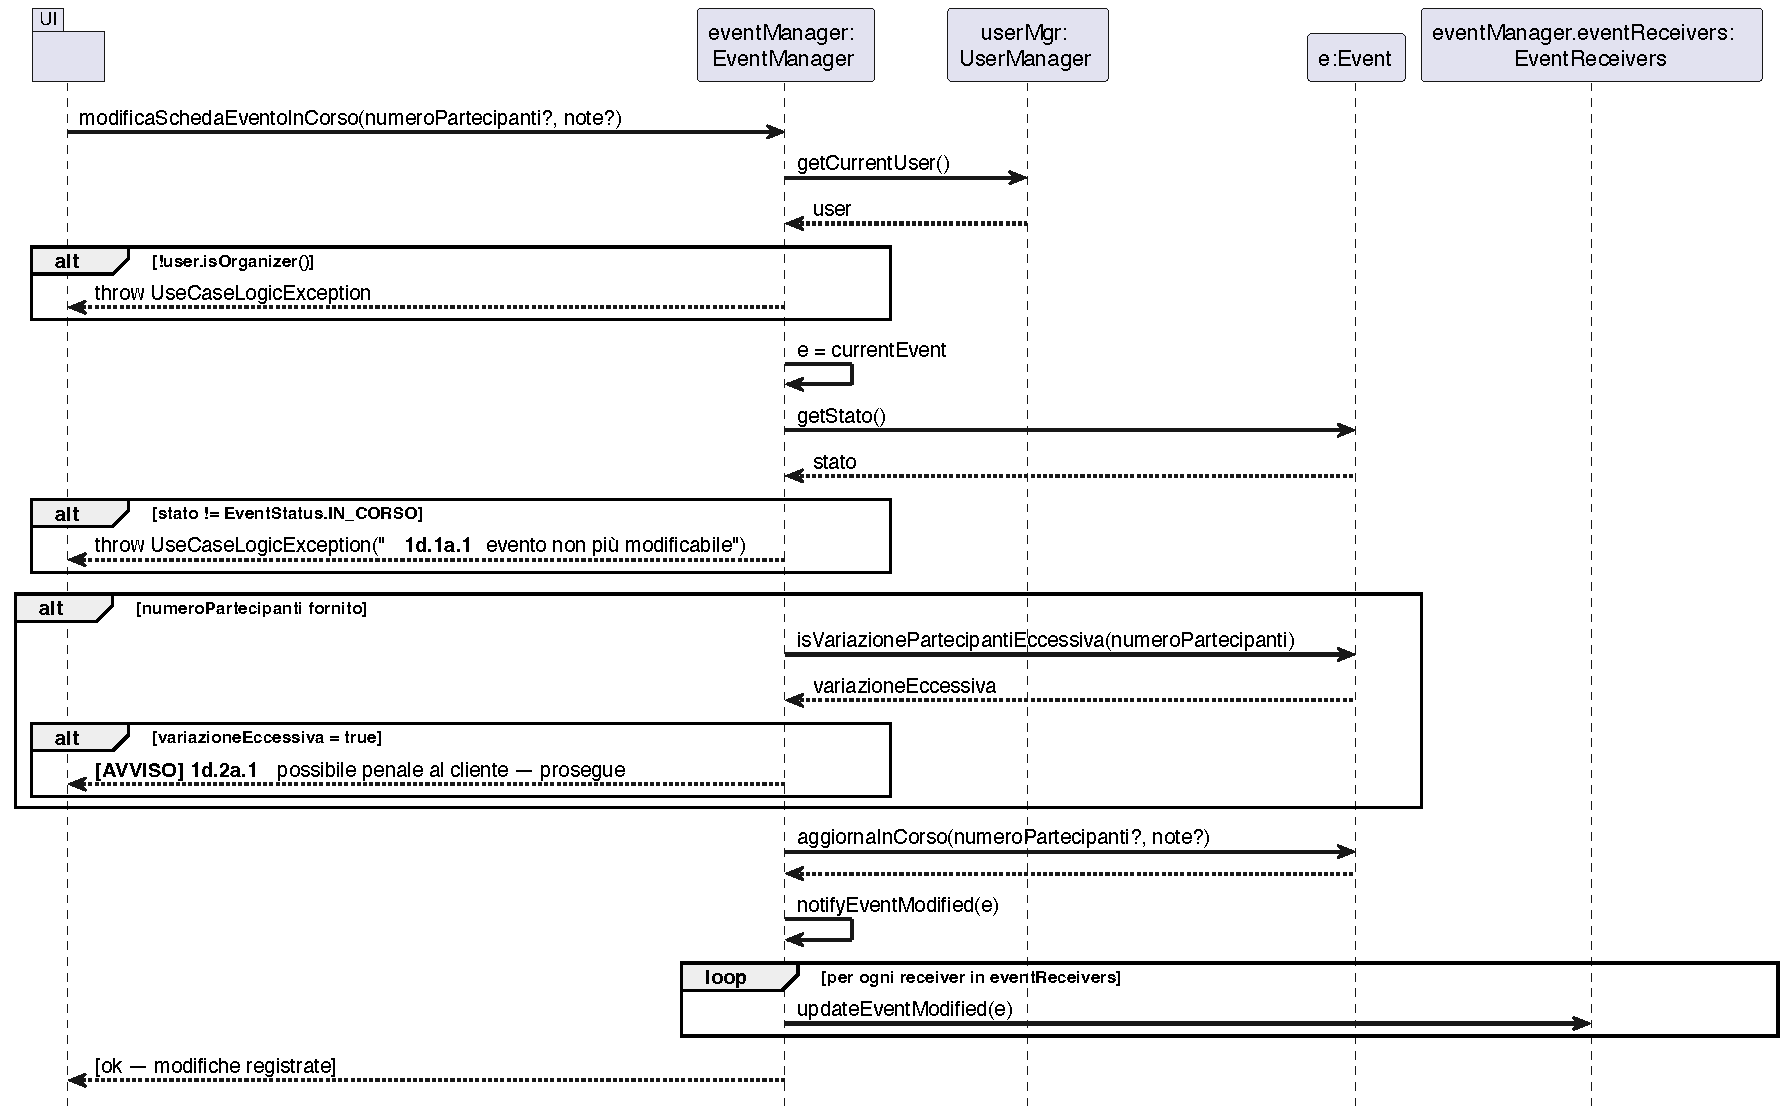
\includegraphics[width=\dsdscreenw, height=\dsdscreenh, keepaspectratio]{dsd/dsd_op15}
\end{figure}

% ─────────────────────────────────────────────────────────────
\clearpage
\dsdpage{595.276}
\section{op14 --- \texttt{consultaMenuServizio}}
\label{sec:dsd_op8}

\begin{figure}[H]
  \centering
  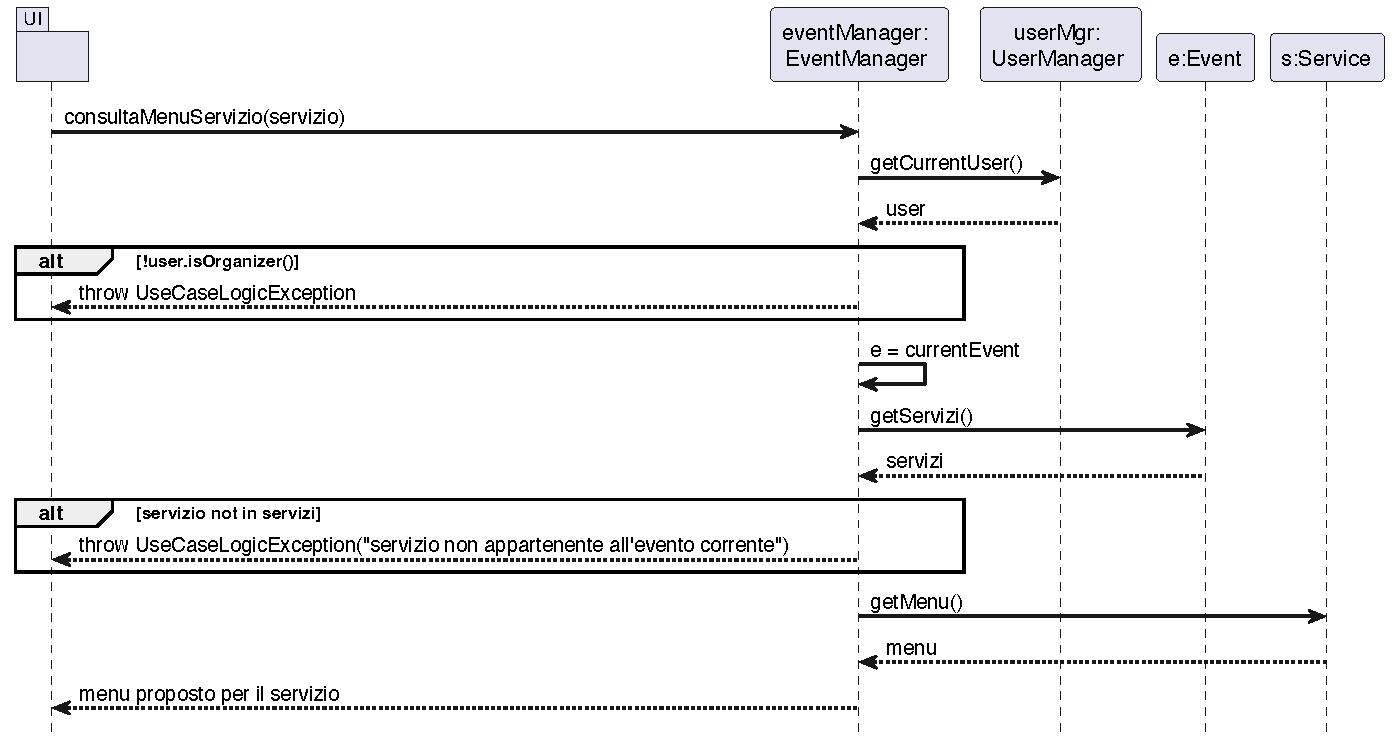
\includegraphics[width=\dsdscreenw, height=\dsdscreenh, keepaspectratio]{dsd/dsd_op8}
\end{figure}

% ─────────────────────────────────────────────────────────────
\clearpage
\dsdpage{595.276}
\section{op15 --- \texttt{proponiModificaMenu}}
\label{sec:dsd_op9}

\begin{figure}[H]
  \centering
  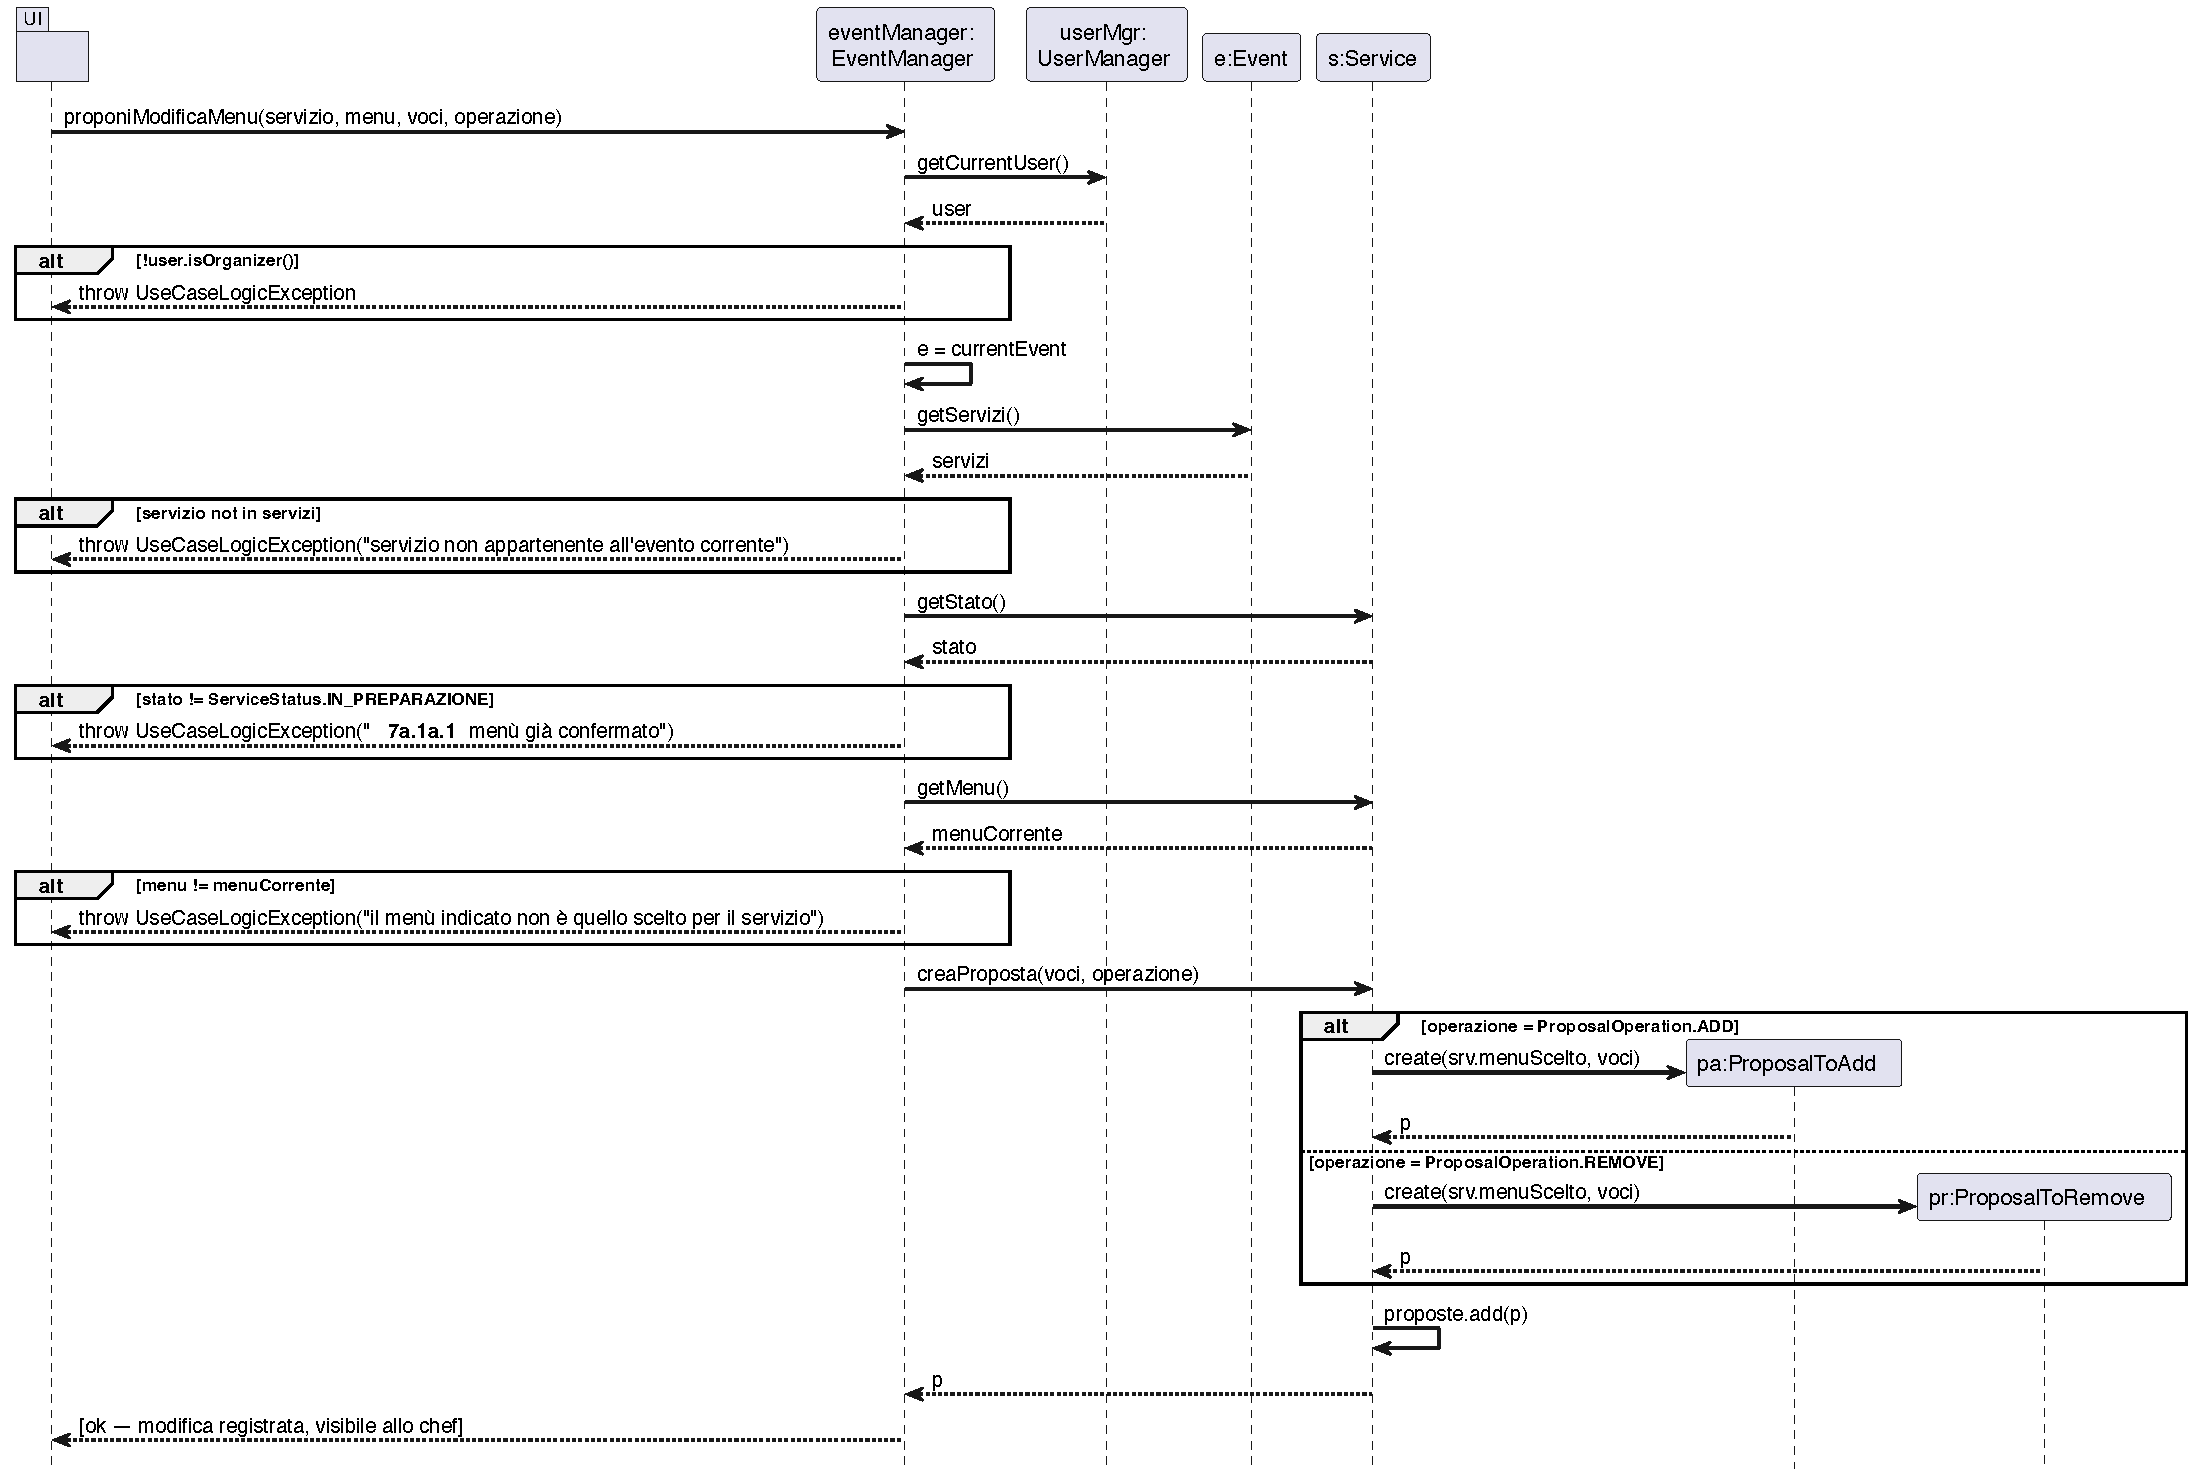
\includegraphics[width=\dsdscreenw, height=\dsdscreenh, keepaspectratio]{dsd/dsd_op9}
\end{figure}

% ─────────────────────────────────────────────────────────────
\clearpage
\dsdpage{595.276}
\section{op16 --- \texttt{assegnaCuocoATurno}}
\label{sec:dsd_op10}

\begin{figure}[H]
  \centering
  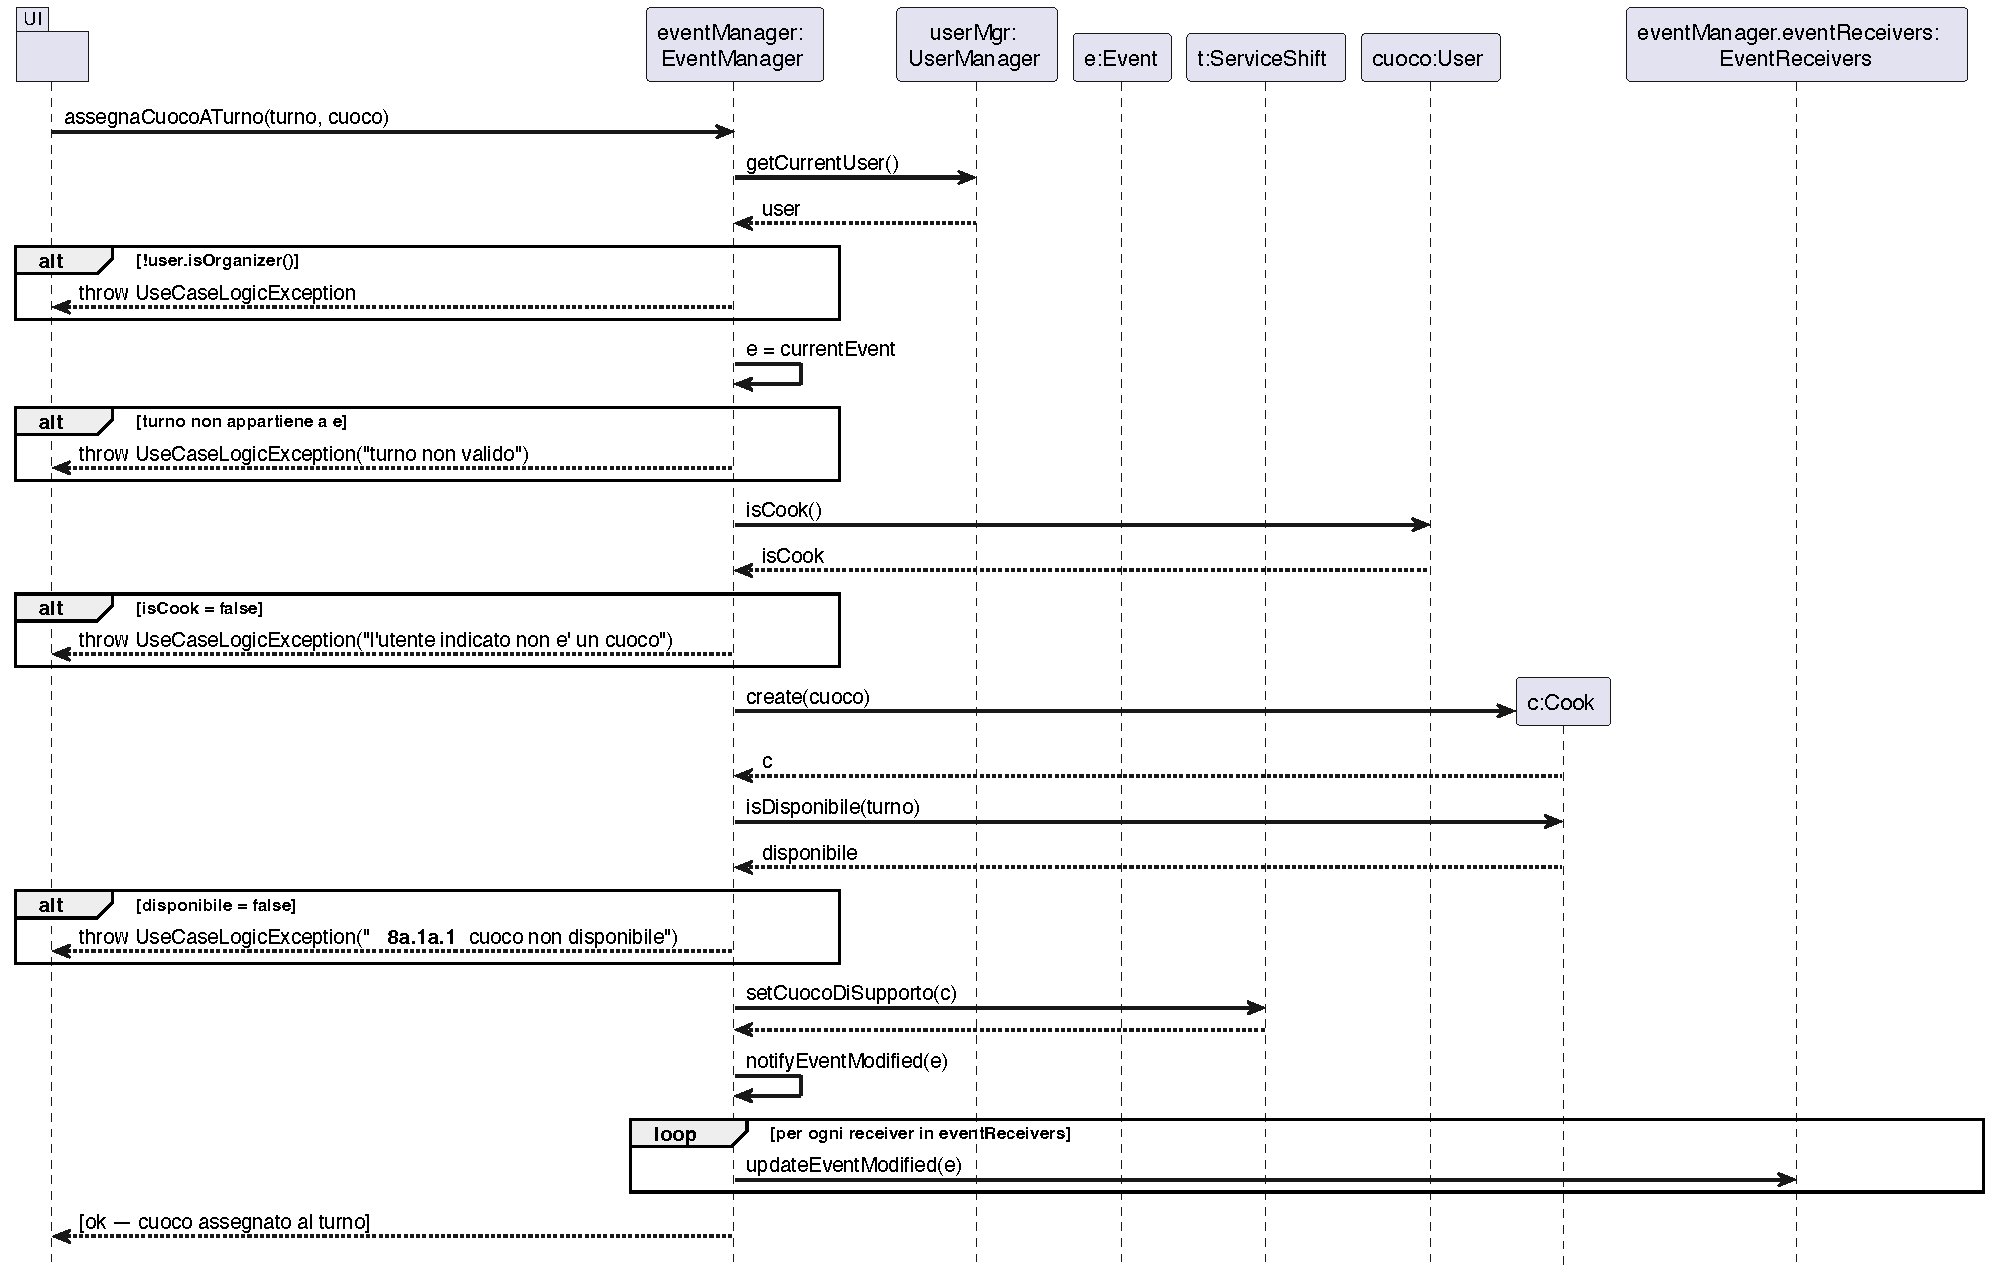
\includegraphics[width=\dsdscreenw, height=\dsdscreenh, keepaspectratio]{dsd/dsd_op10}
\end{figure}

% ─────────────────────────────────────────────────────────────
\clearpage
\dsdpage{595.276}
\section{op17 --- \texttt{rimuoviPersonaleDaTurno}}
\label{sec:dsd_op11}

\begin{figure}[H]
  \centering
  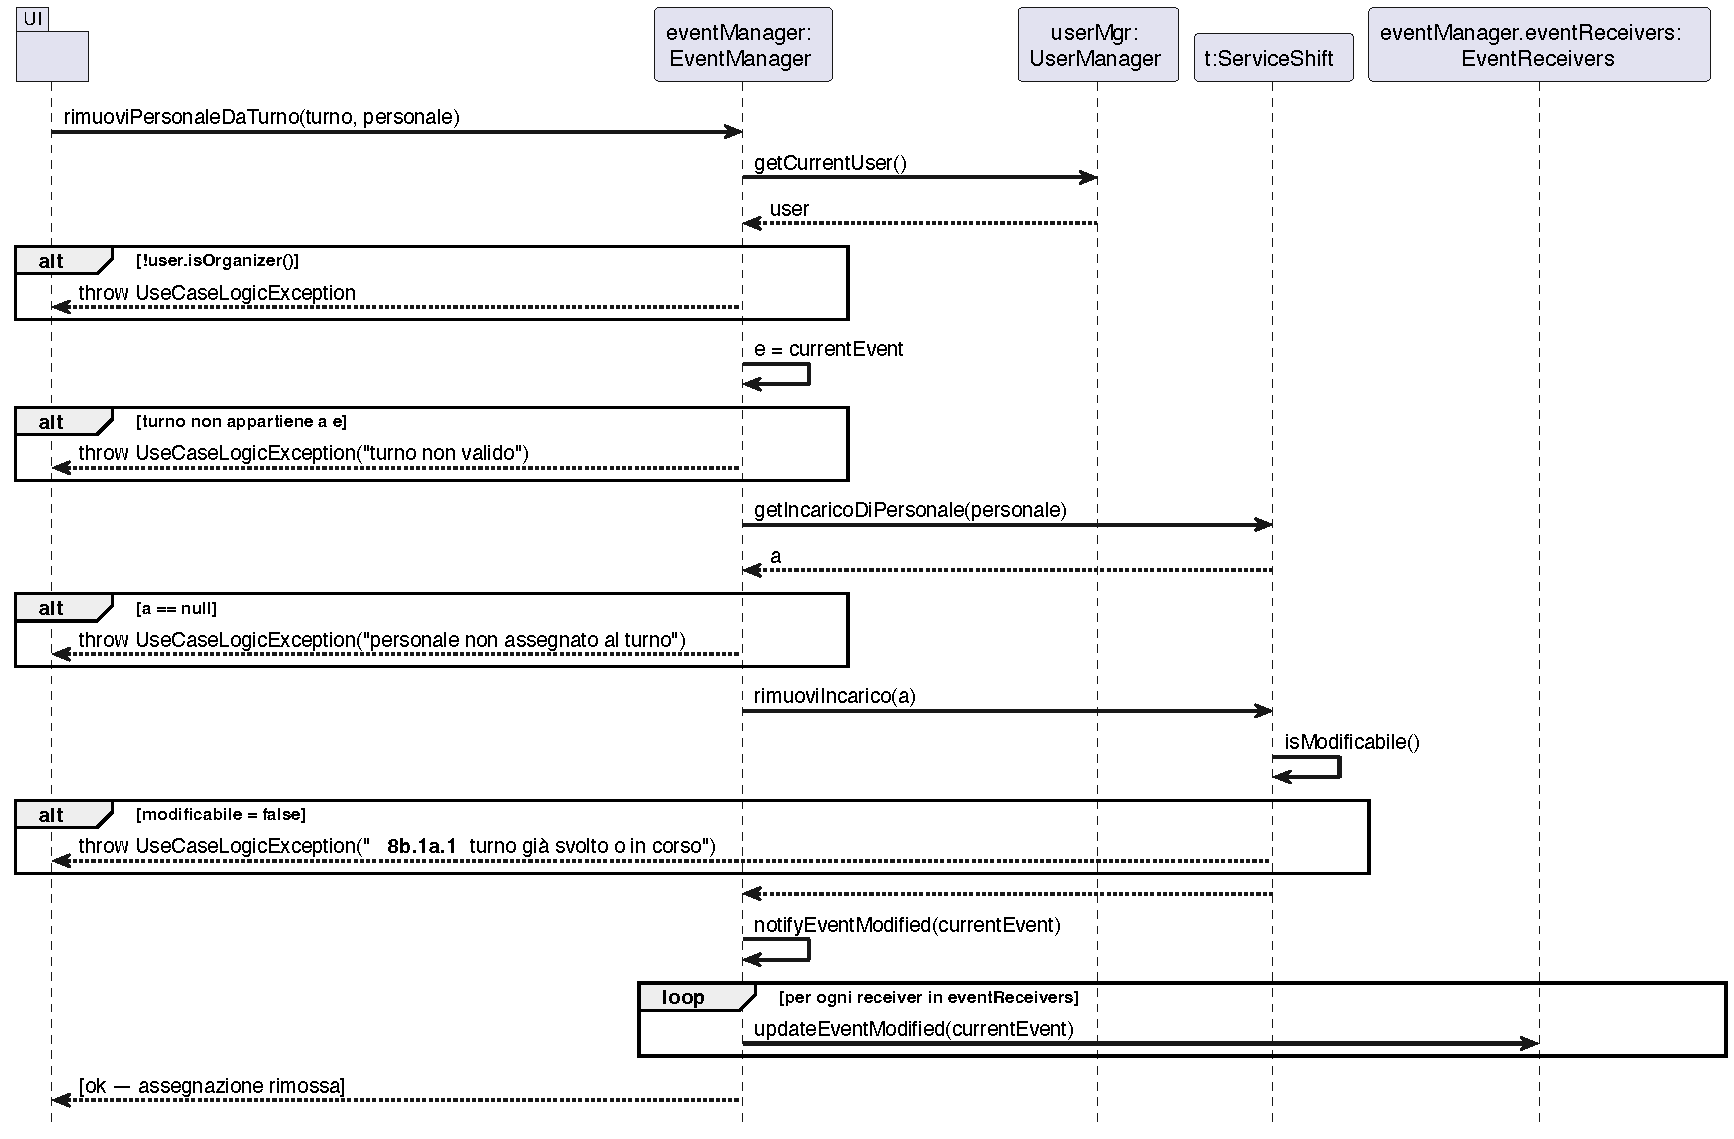
\includegraphics[width=\dsdscreenw, height=\dsdscreenh, keepaspectratio]{dsd/dsd_op11}
\end{figure}

% ─────────────────────────────────────────────────────────────
\clearpage
\dsdpage{595.276}
\section{op18 --- \texttt{selezionaIstanza}}
\label{sec:dsd_op19}

\begin{figure}[H]
  \centering
  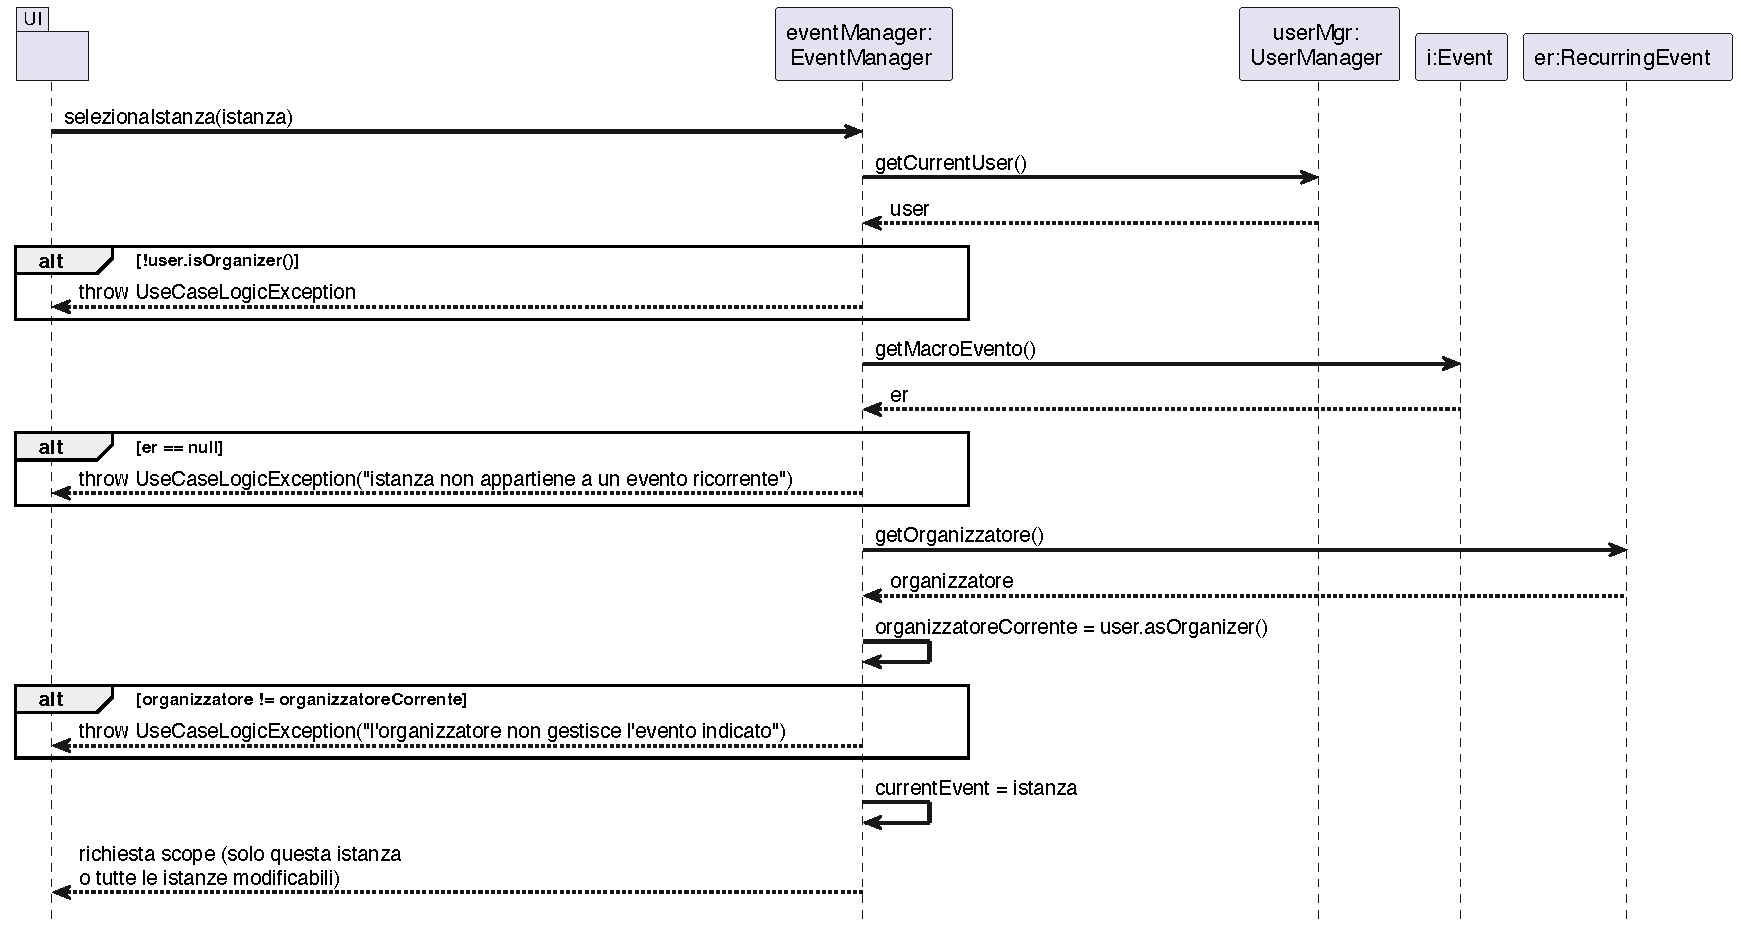
\includegraphics[width=\dsdscreenw, height=\dsdscreenh, keepaspectratio]{dsd/dsd_op19}
\end{figure}

% ─────────────────────────────────────────────────────────────
\clearpage
\dsdpage{730}
\section{op19 --- \texttt{operaSuIstanza}}
\label{sec:dsd_op12}

\begin{figure}[H]
  \centering
  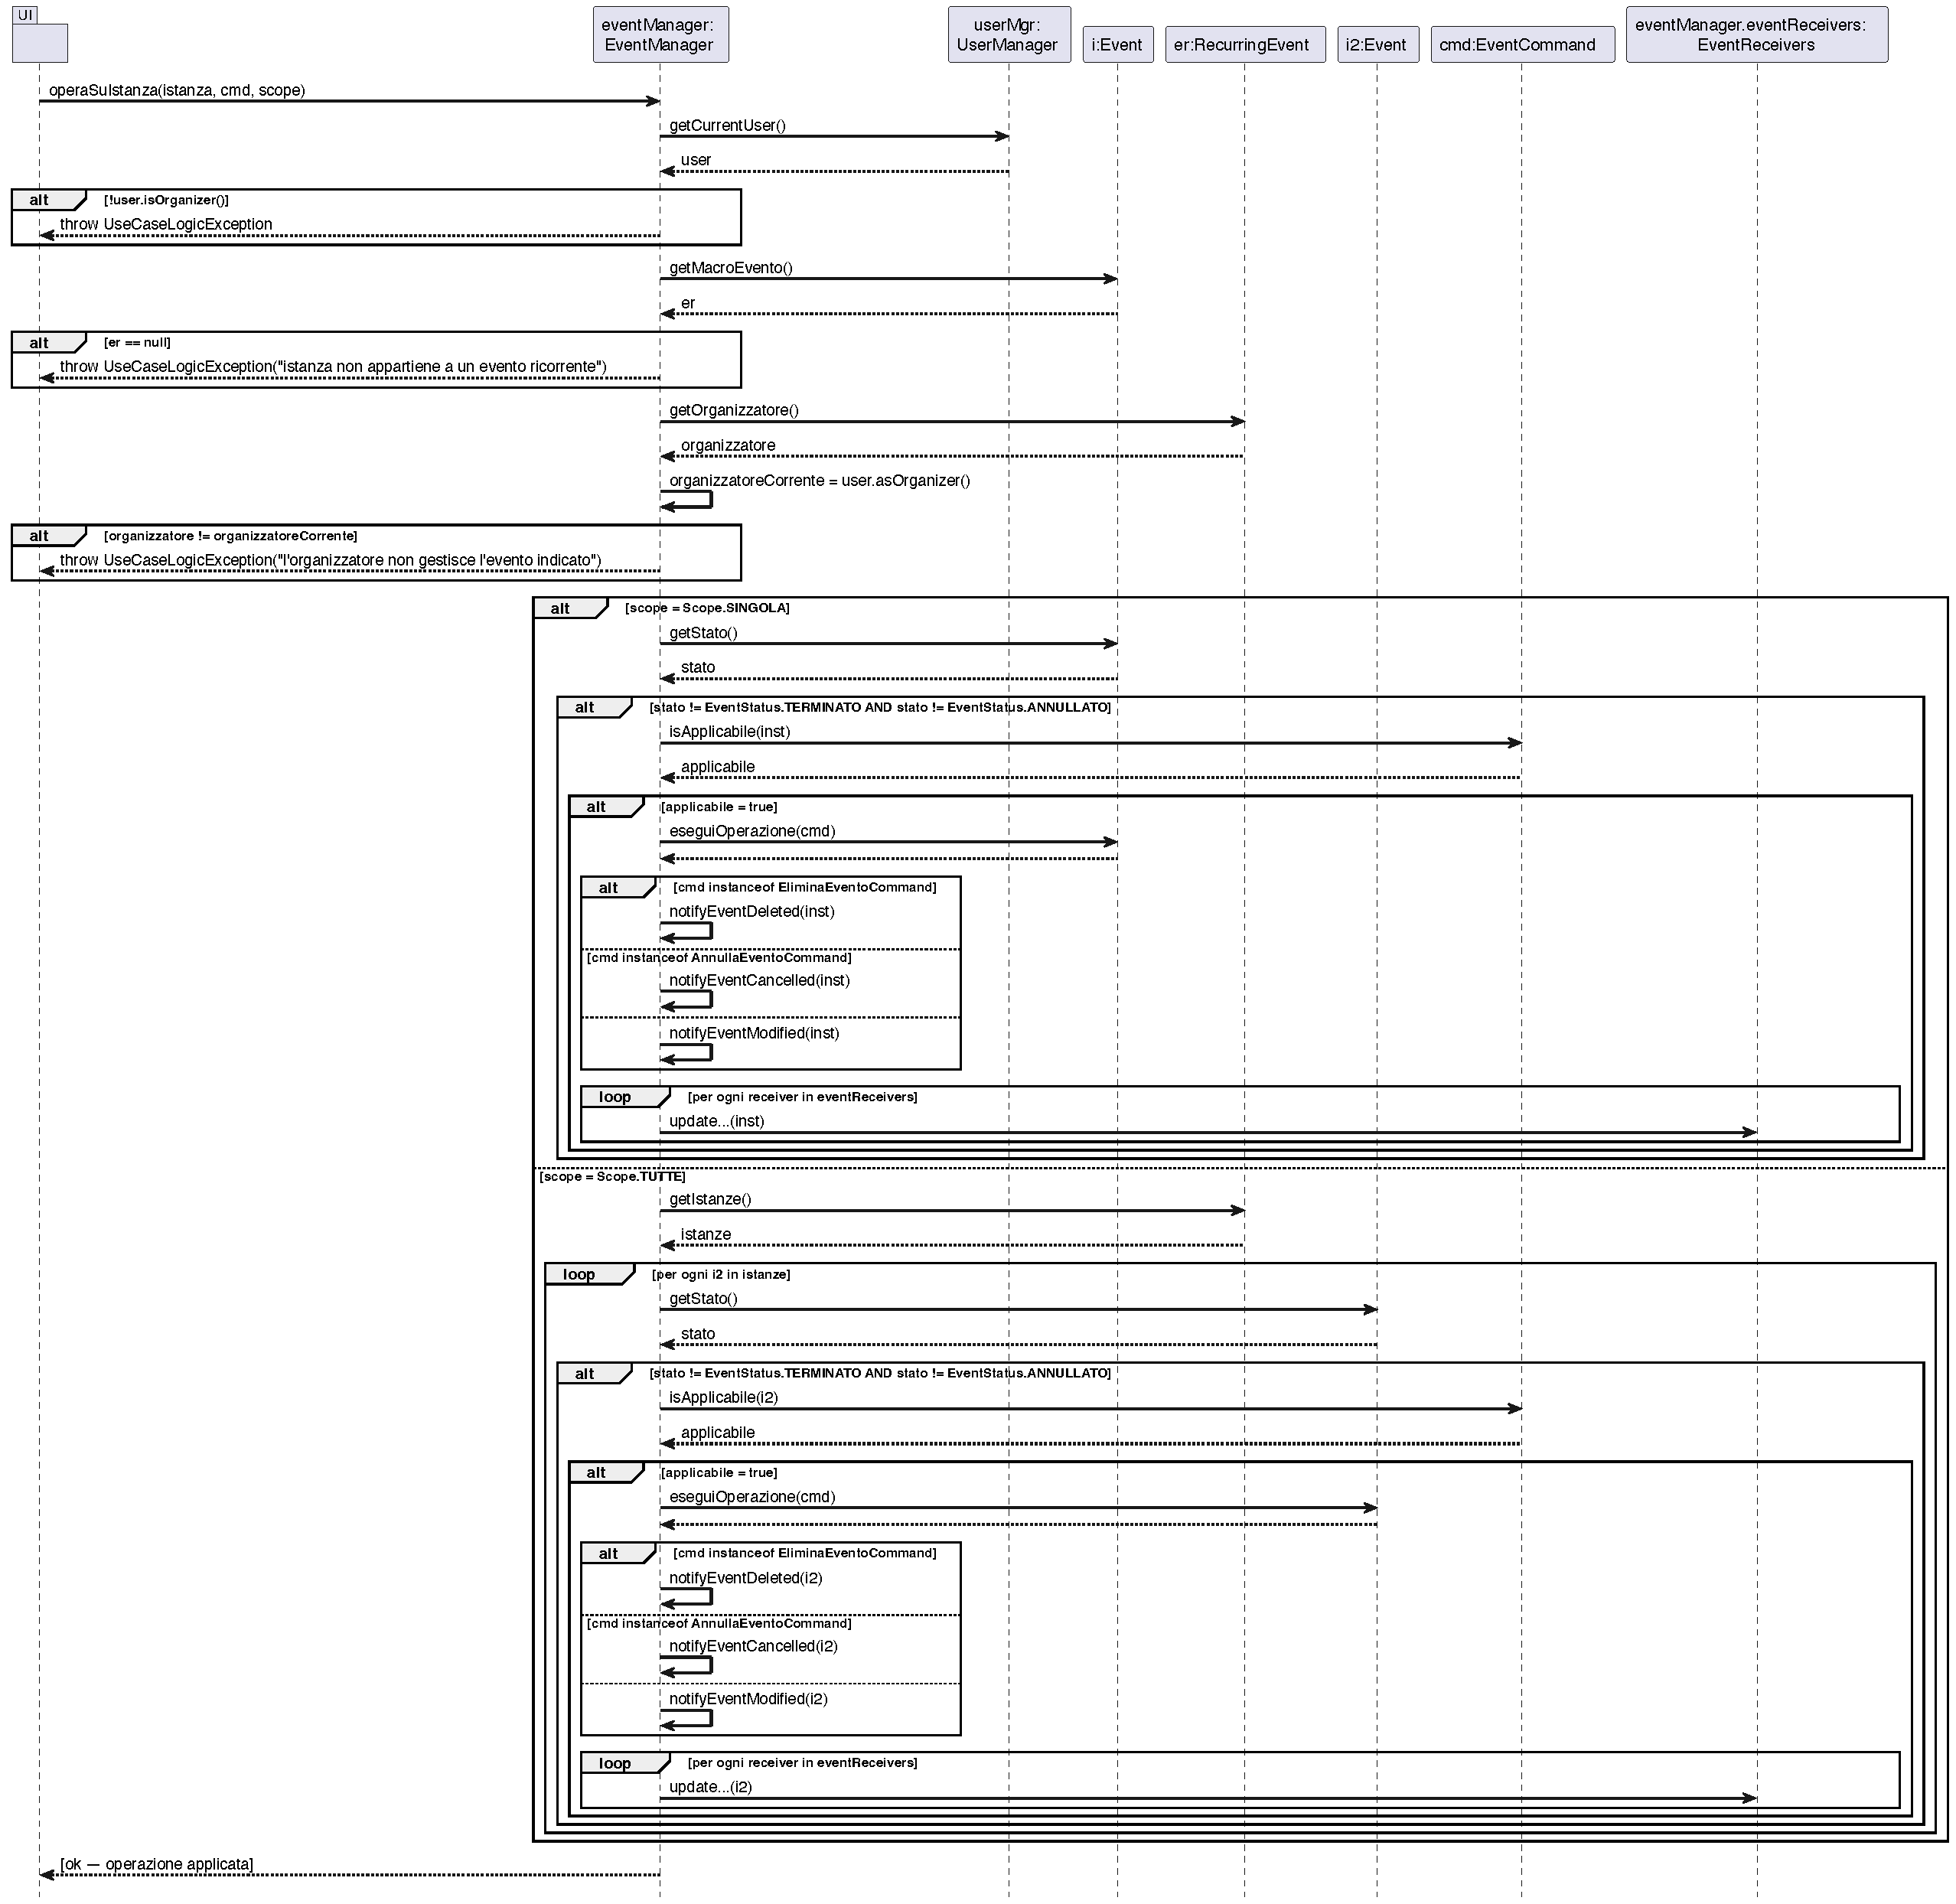
\includegraphics[width=\dsdscreenw, height=606pt, keepaspectratio]{dsd/dsd_op12}
\end{figure}

% ─────────────────────────────────────────────────────────────
\clearpage
\dsdpage{730}
\section{op20 --- \texttt{modificaRicorrenza}}
\label{sec:dsd_op13}

\begin{figure}[H]
  \centering
  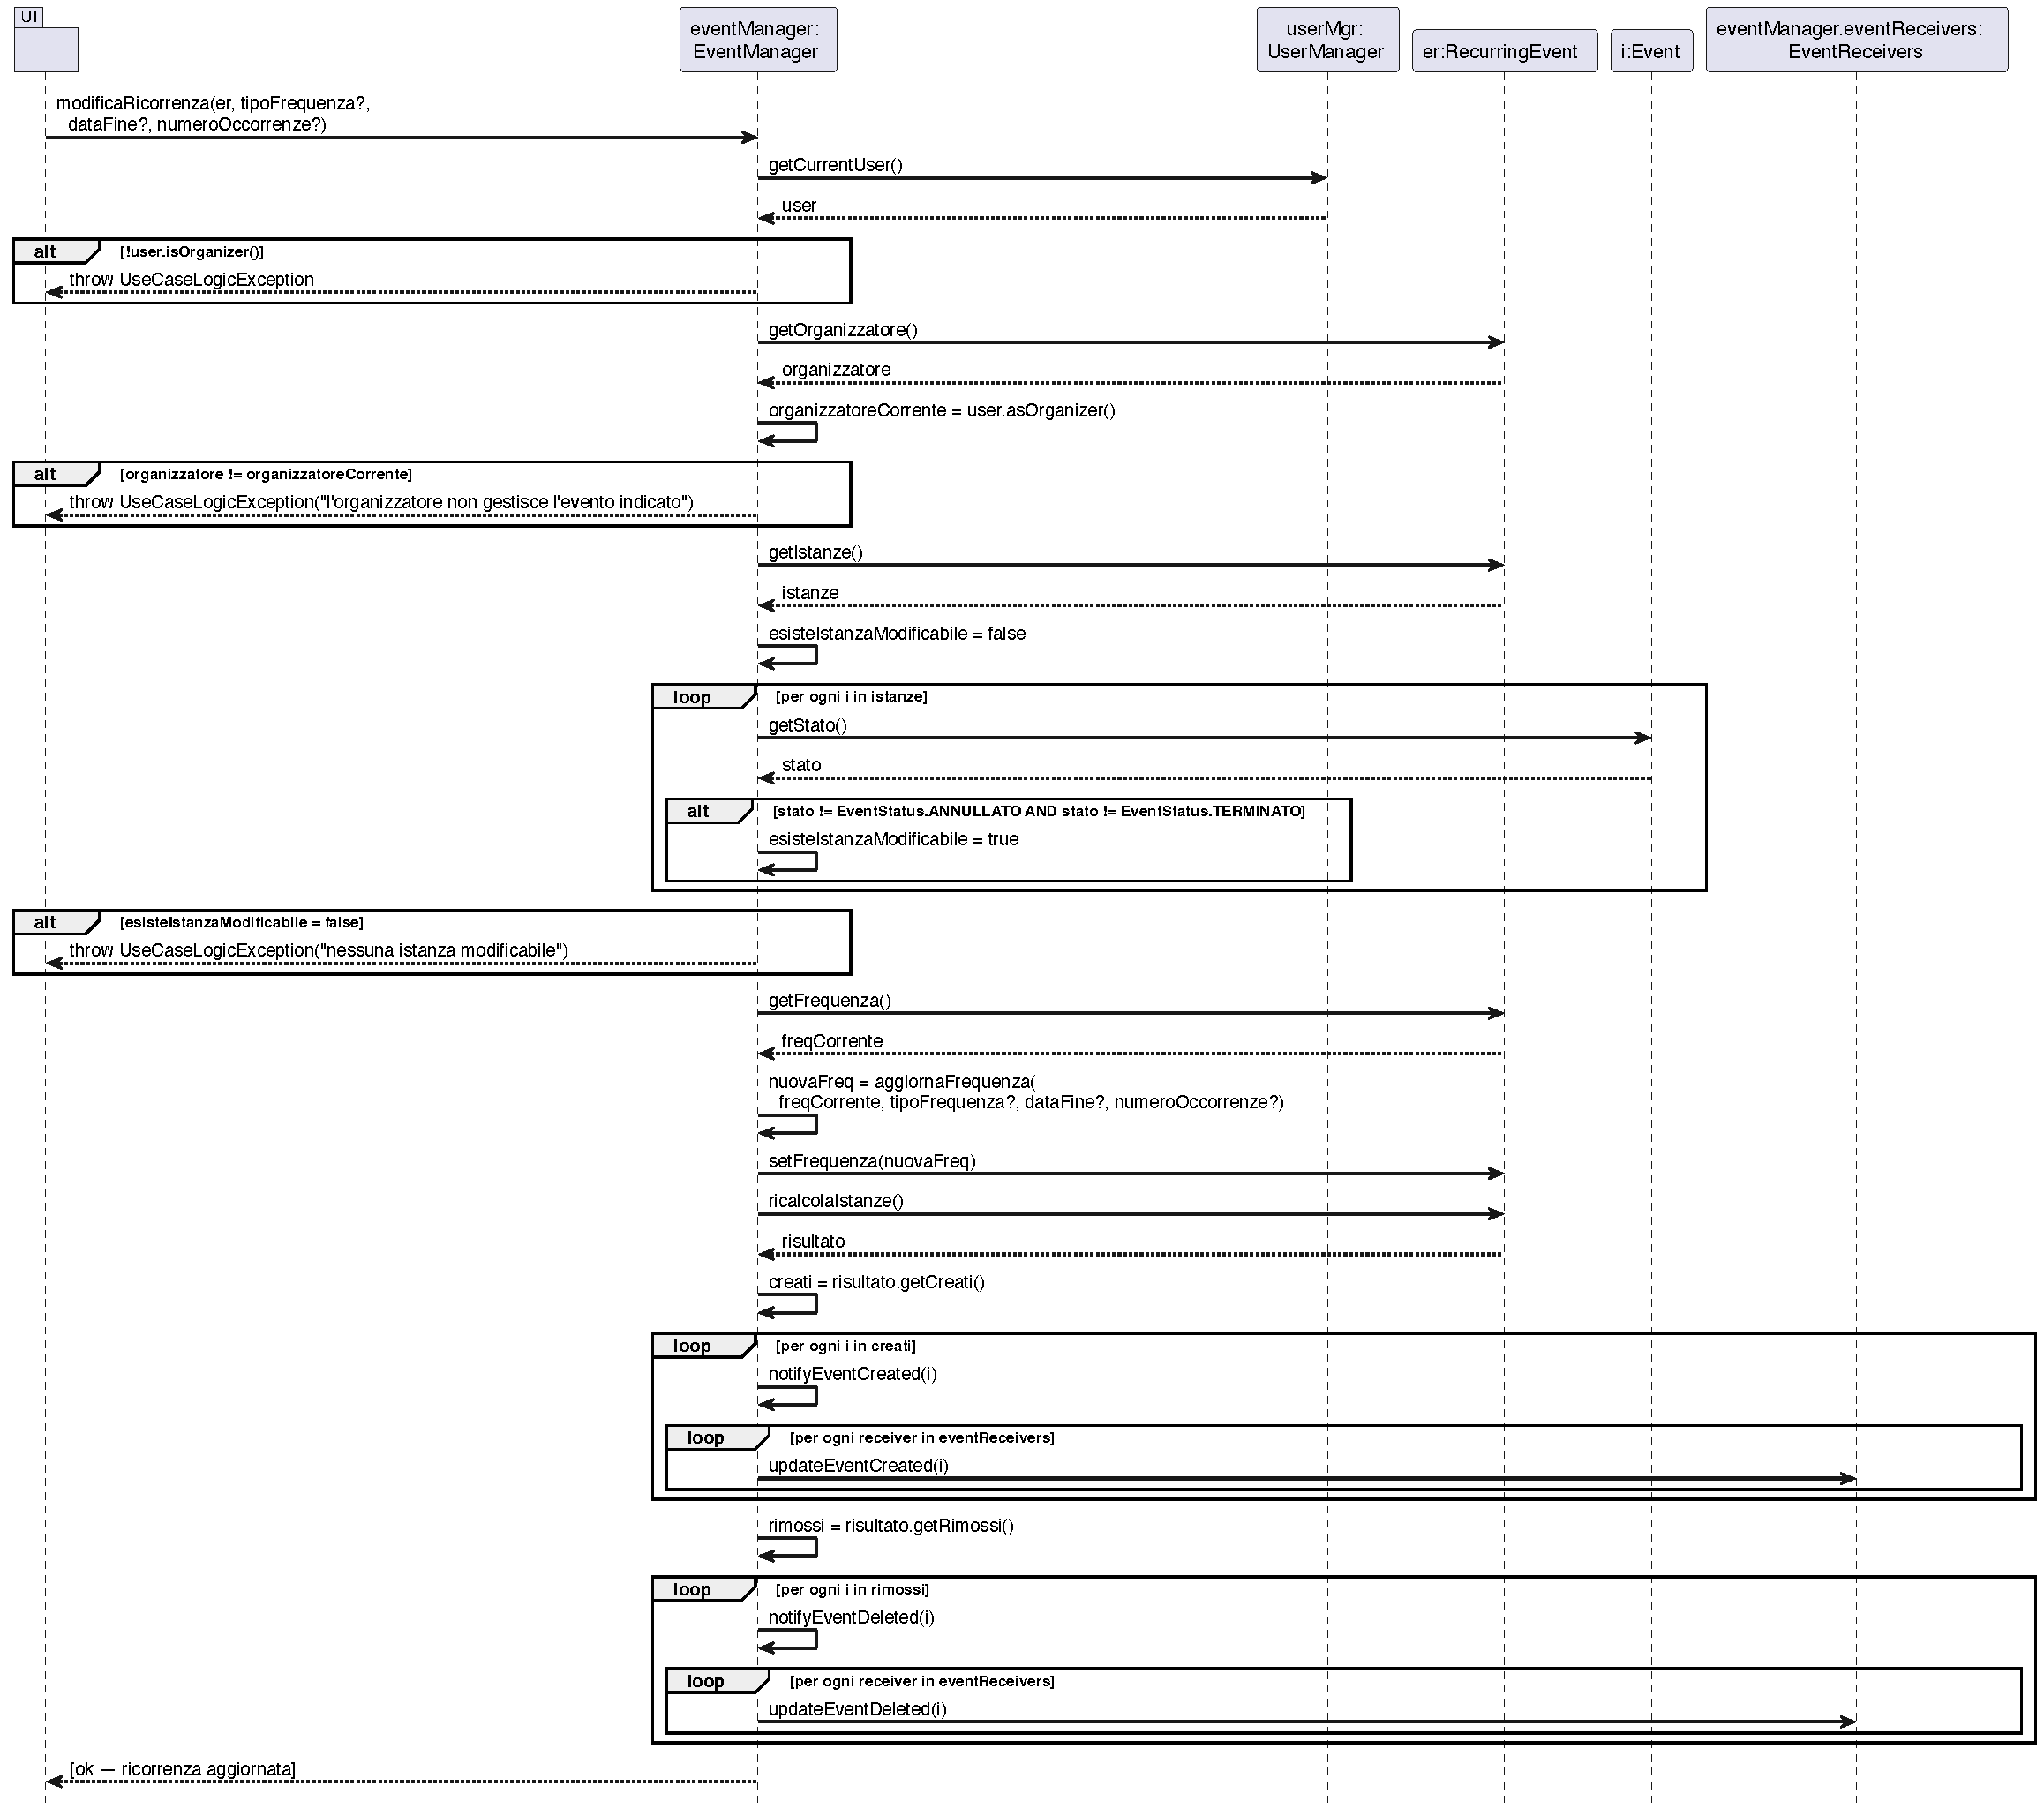
\includegraphics[width=\dsdscreenw, height=606pt, keepaspectratio]{dsd/dsd_op13}
\end{figure}

% ─────────────────────────────────────────────────────────────
\clearpage
\dsdpage{595.276}
\section{op21 --- \texttt{annullaServizio}}
\label{sec:dsd_op14}

\begin{figure}[H]
  \centering
  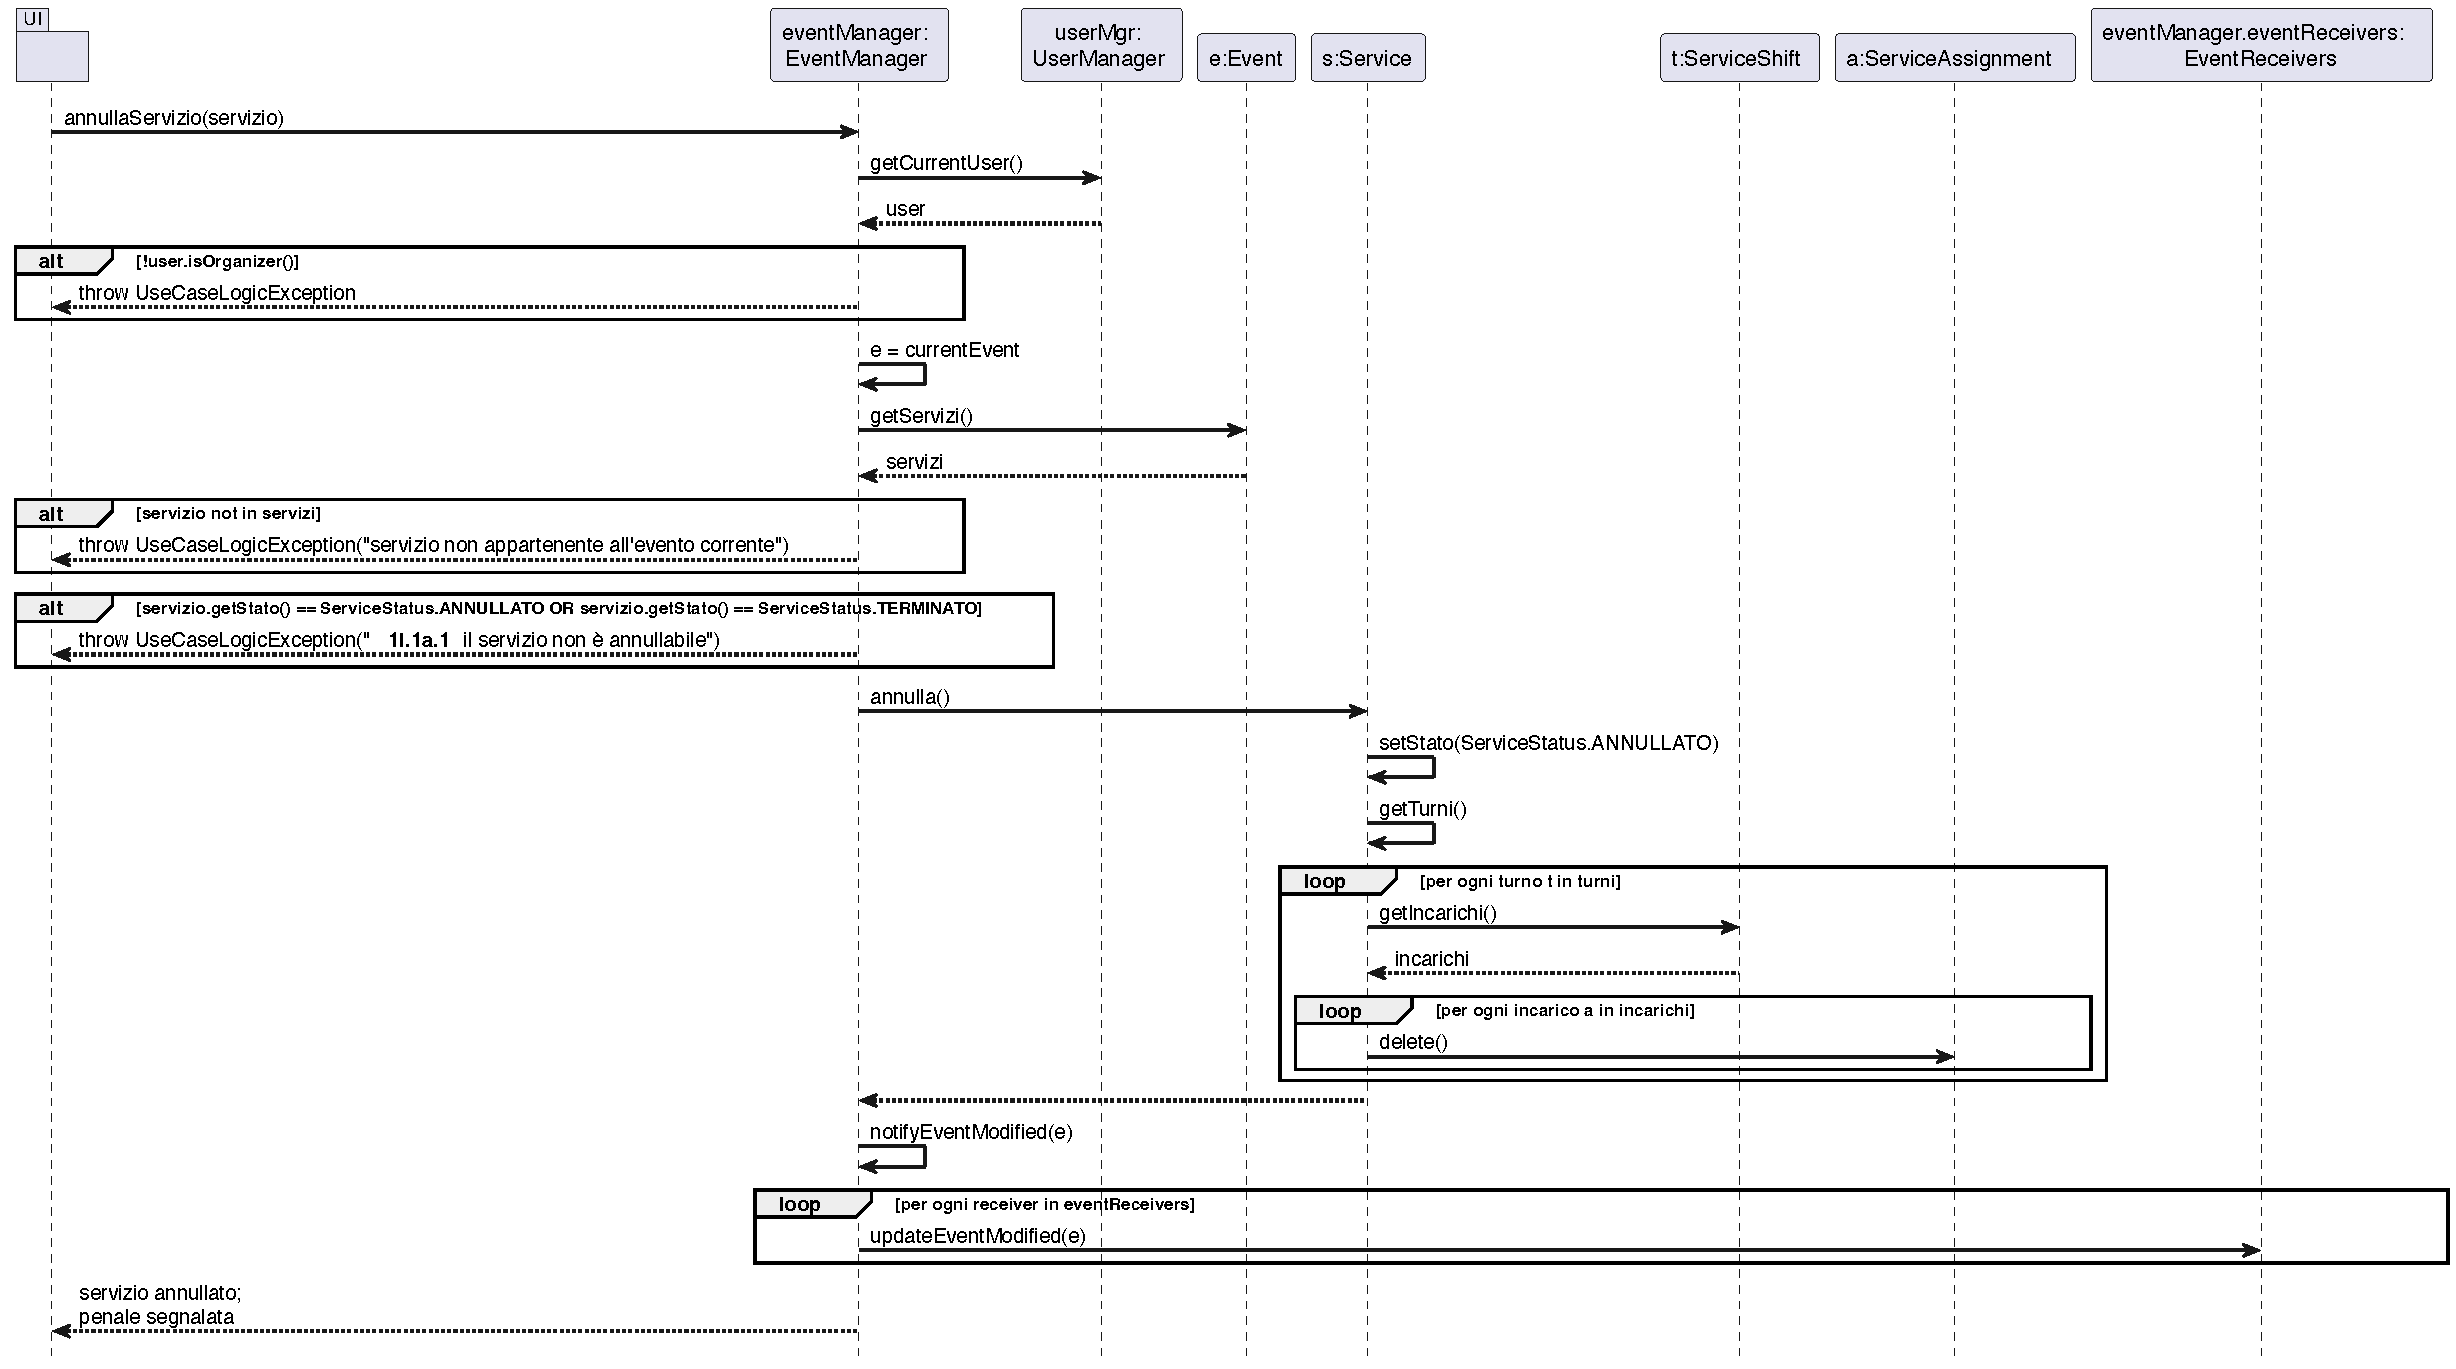
\includegraphics[width=\dsdscreenw, height=\dsdscreenh, keepaspectratio]{dsd/dsd_op14}
\end{figure}

\clearpage
\dsdrestorepage


\end{document}
